\newpage
\graphicspath{{../giaitoancungbi/mitdac/}}
\begingroup
\AddToShipoutPicture*{\put(96,595){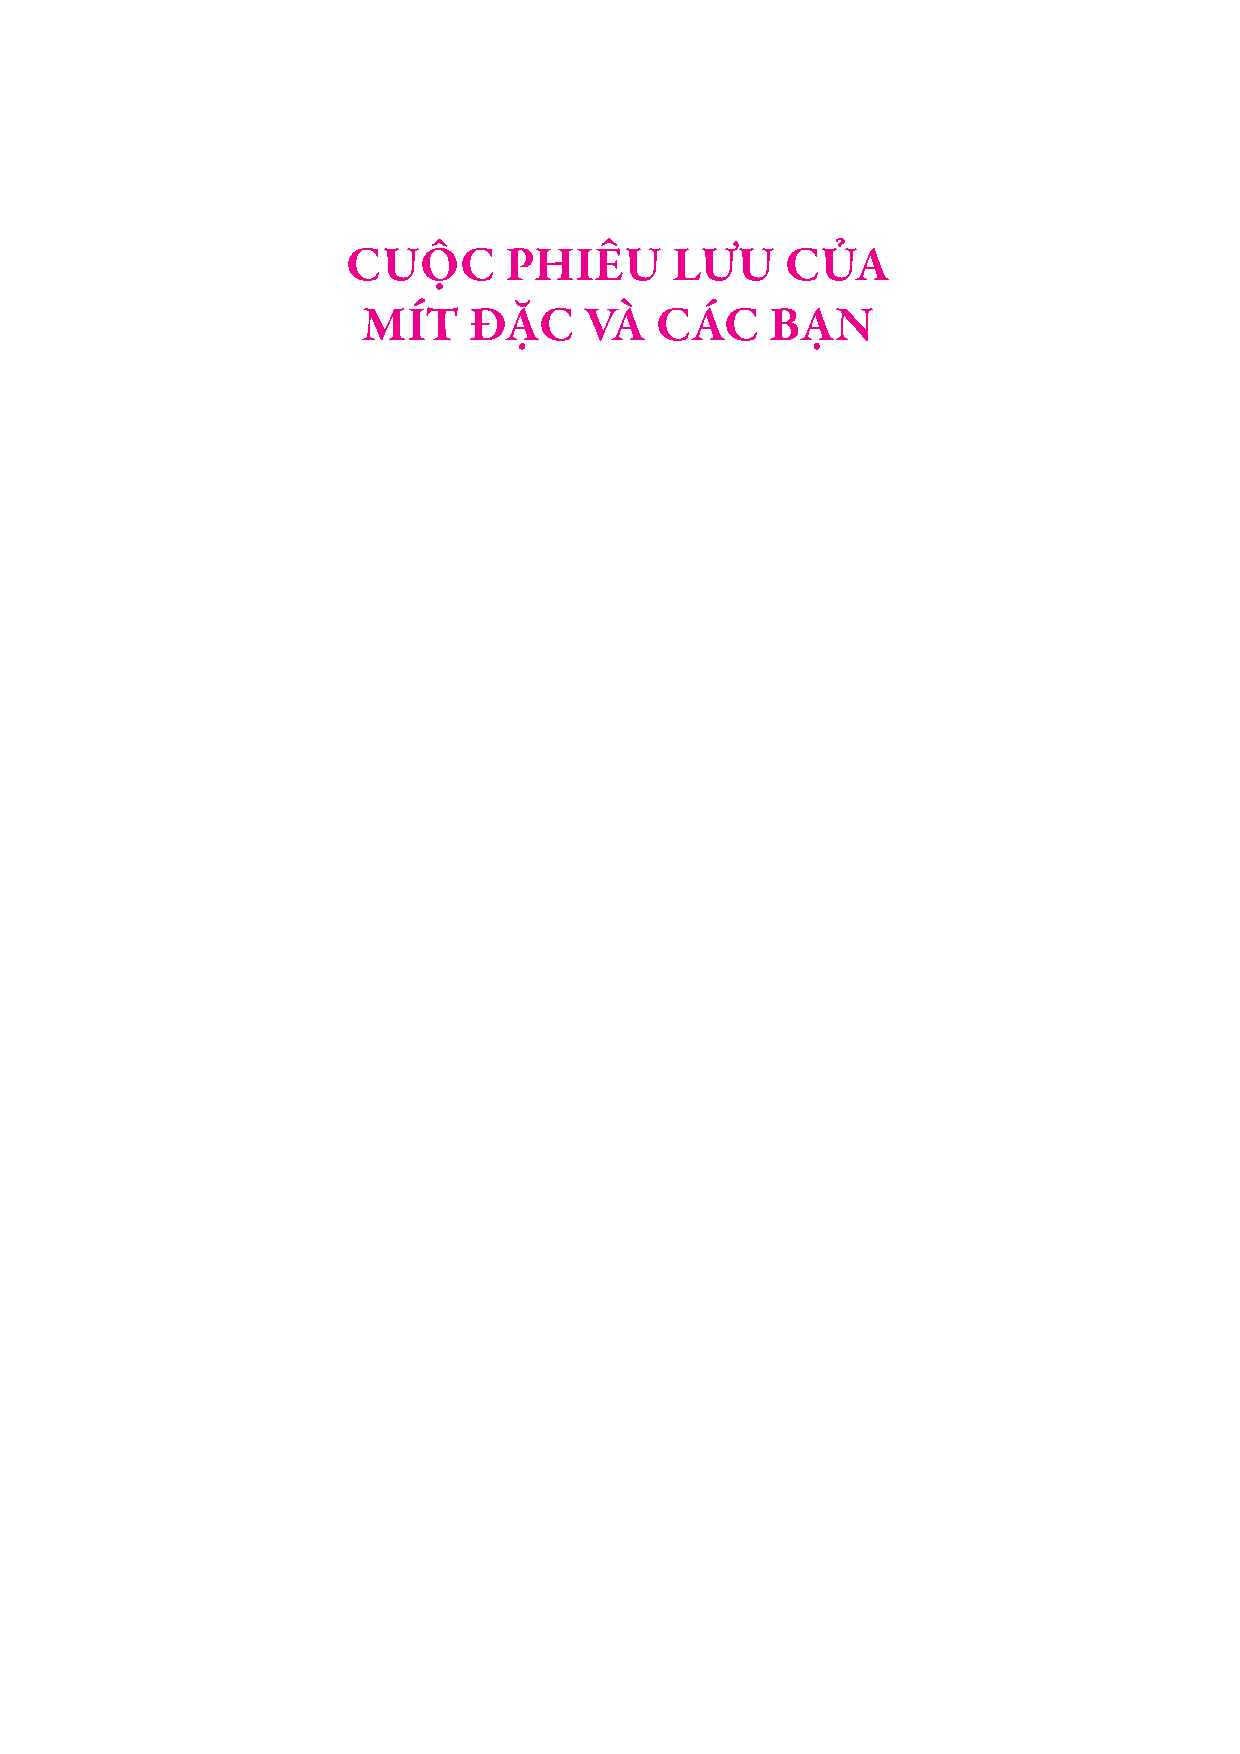
\includegraphics[scale=1]{../mitdac/tieude.pdf}}} % %Image background
\centering
\endgroup
\vspace*{25pt}

	\begin{multicols}{2}
		\textit{Những bạn nhỏ đã đọc “Chuyện phiêu lưu của Mít Đặc và các bạn” thì đã biết đến Mít Đặc và các cô chú tí hon hết sức tinh nghịch và ngộ ngĩnh, sống ở những thành phố nhỏ bé nhưng vô cùng đẹp đẽ và đáng yêu. Các cô chú luôn hăng say lao động, chế tạo ra những máy móc kì lạ, làm thơ, ca hát, thích khám phá những vùng đất mới mẻ, ...}
		\begin{figure}[H]
			\centering
			\vspace*{5pt}
			\captionsetup{labelformat= empty, justification=centering}
			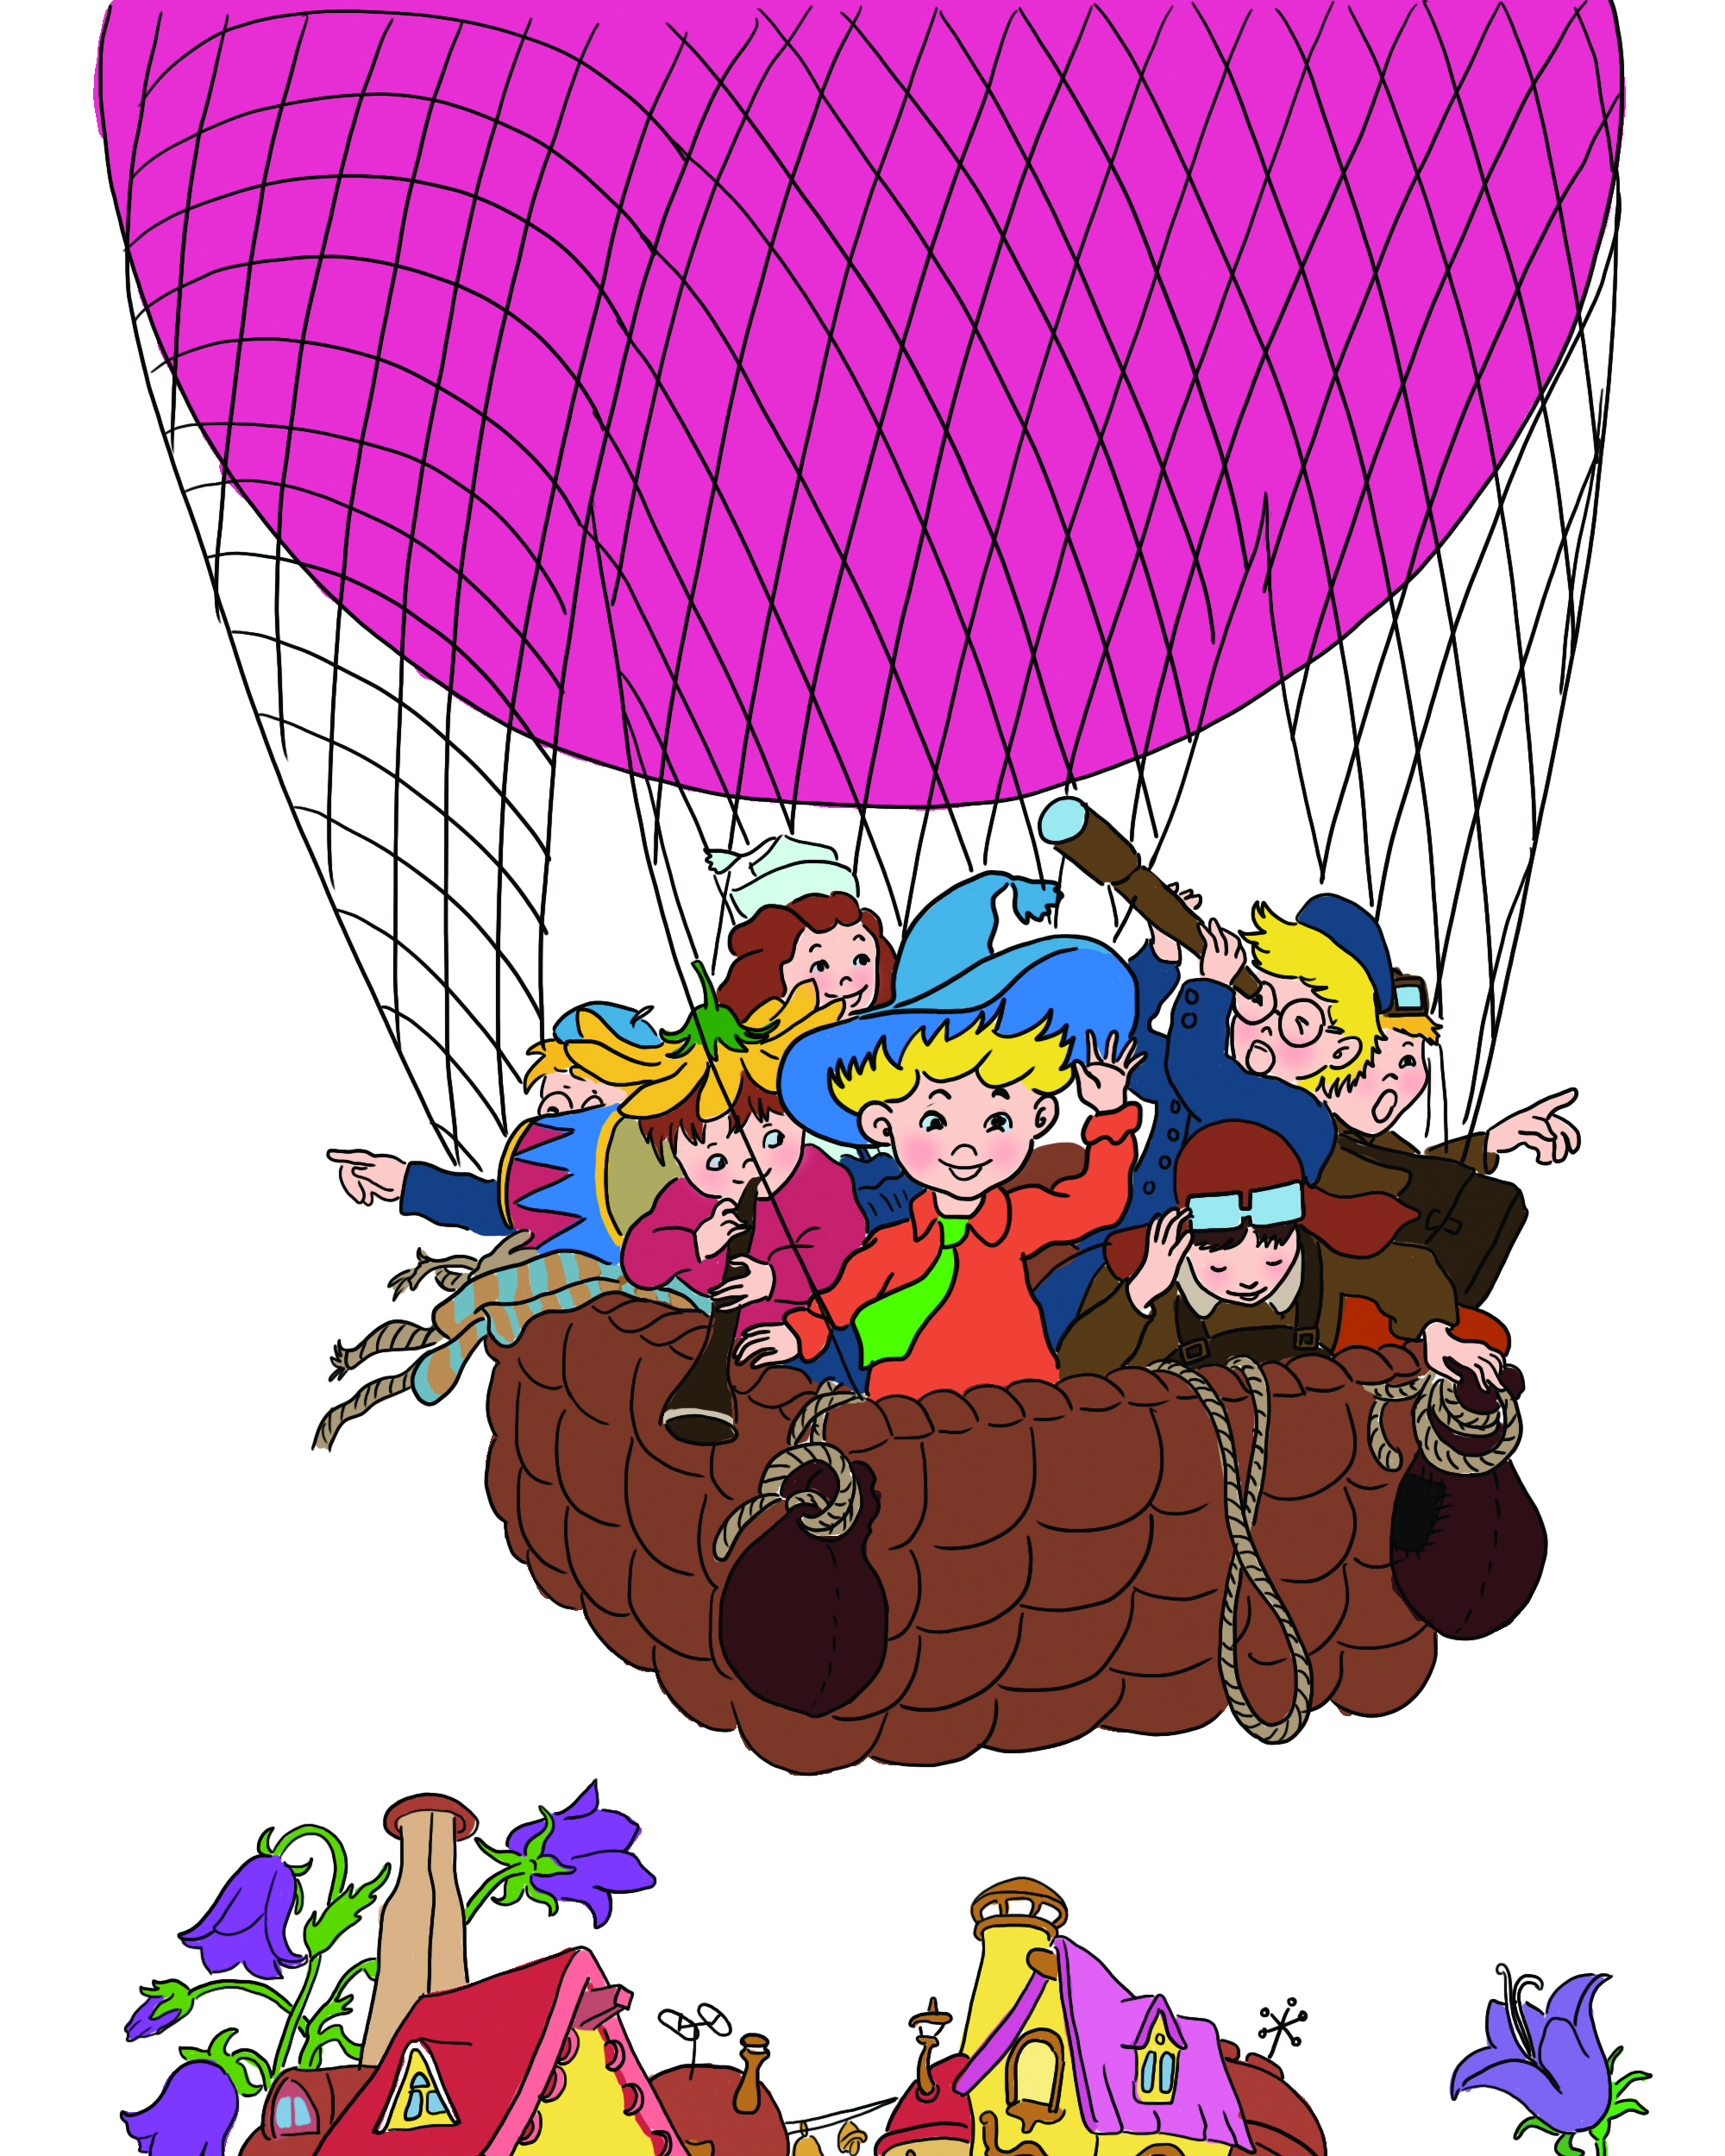
\includegraphics[width=0.9\linewidth]{Hinh0}
			%\caption{\textit{\color{toancuabi}Hình $1$. Thành phố Hoa}}
			\vspace*{-10pt}
		\end{figure}
	\end{multicols}
	Trong phần này, chúng ta sẽ gặp lại Mít Đặc và các cô chú tí hon dễ thương, phiêu lưu cùng các cô chú qua những bài toán đố vui vẻ và thú vị sau nhé.
	\begin{center}
		\textbf{\color{toancuabi}Những người bạn ở thành phố Hoa}
	\end{center}
	\begin{multicols}{2}
		\textit{Mít Đặc và những người bạn sống ở một thành phố rất đẹp, đẹp như một thành phố trong truyện thần tiên. Xung quanh những ngôi nhà mọc đủ các loại hoa: hoa mẫu đơn, hoa cúc, hoa lan và các phố xá cũng mang những tên hoa: Hoa Bìm Bìm, phố Hoa Cúc, phố Hoa Mua. Còn thành phố được gọi là thành phố Hoa, nằm bên bờ suối mà các côn chú tí hon gọi là sông Dưa Chuột vì hai bên bờ mọc rất nhiều dưa chuột.}
		\begin{figure}[H]
			\centering
			\vspace*{-5pt}
			\captionsetup{labelformat= empty, justification=centering}
			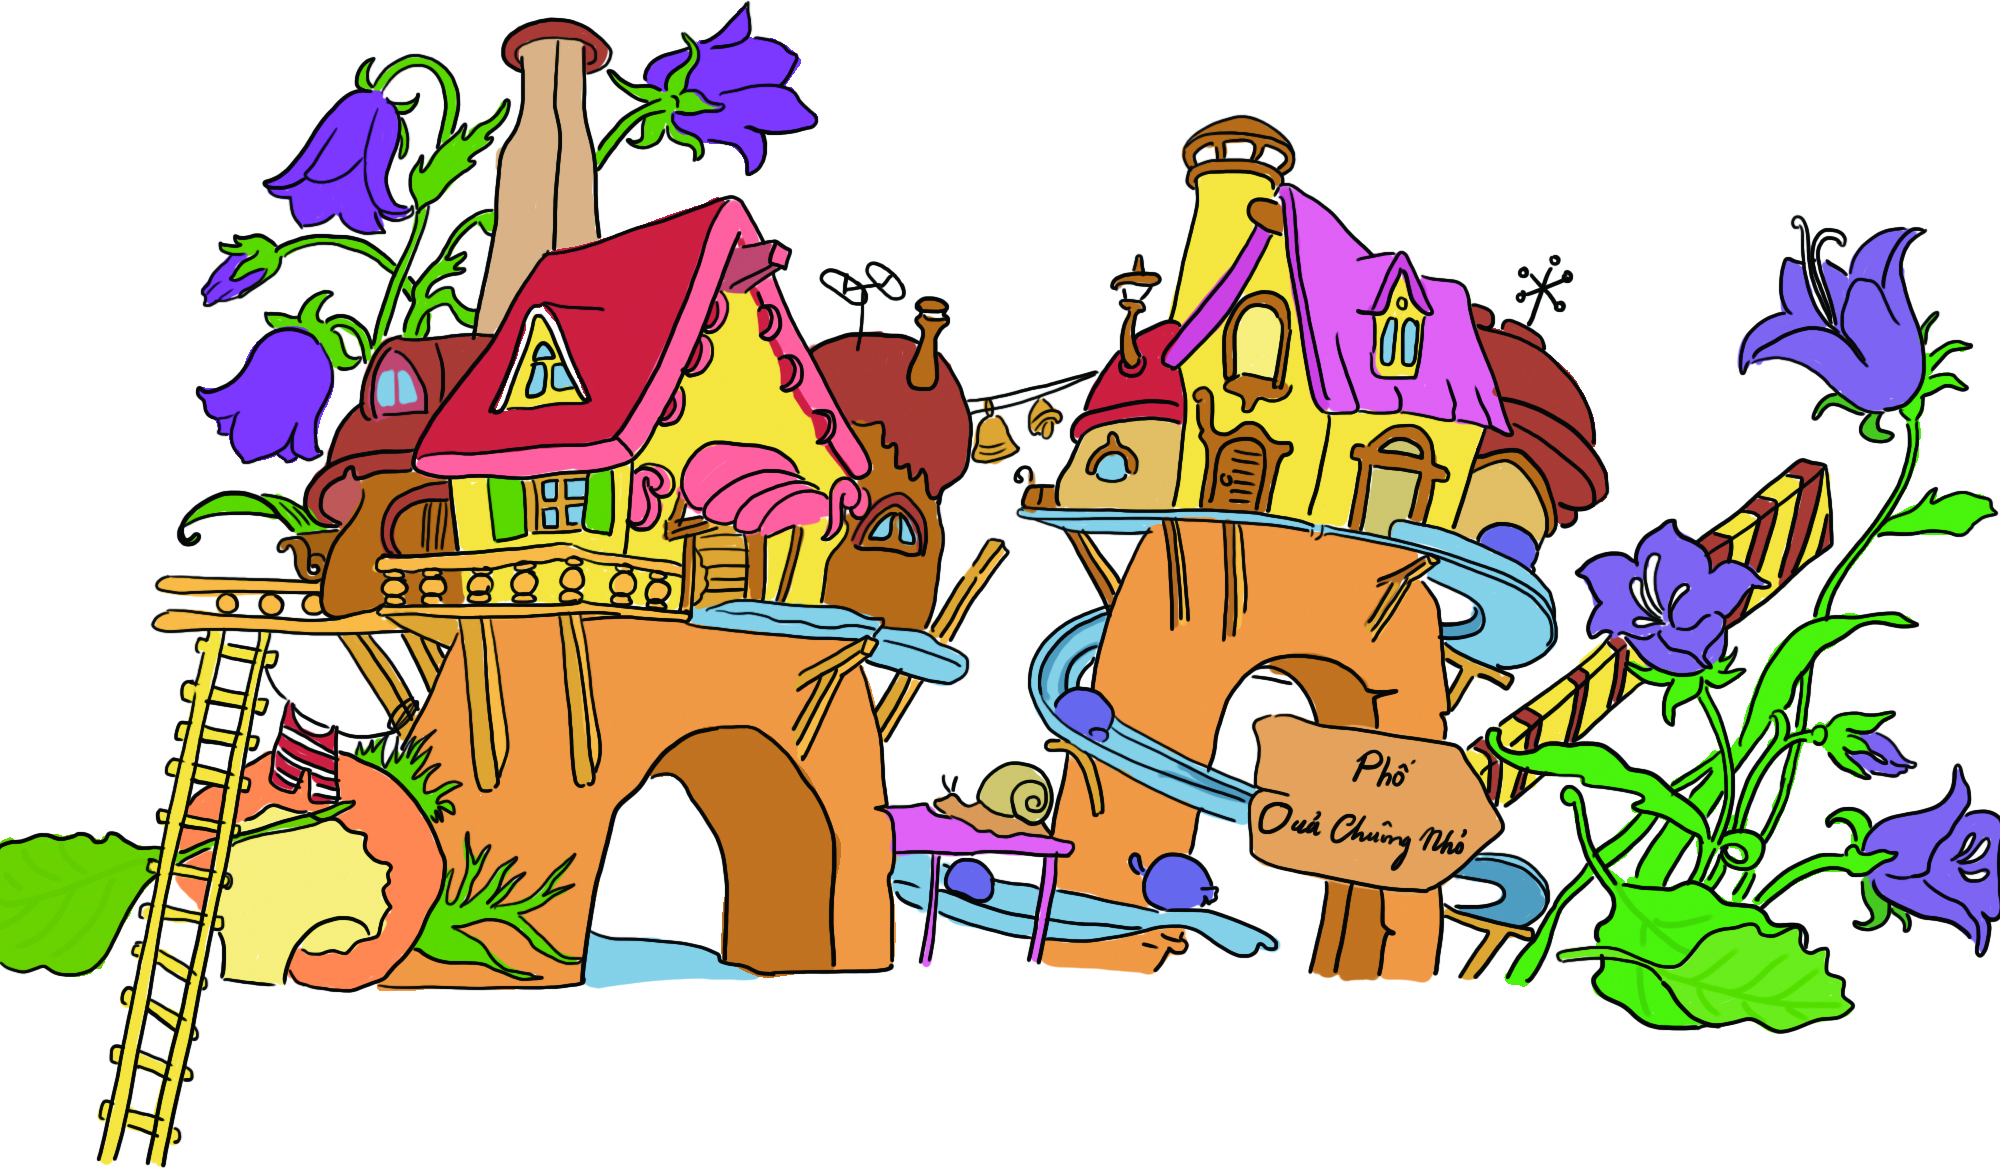
\includegraphics[width=1\linewidth]{Hinh1_TPHoa}
			\vspace*{-5pt}
		\end{figure}
	\end{multicols}
	Mít Đặc cùng $15$ chú tí hon khác ở cùng trong một ngôi nhà ở phố Hoa Bìm Bìm. Chúng ta hãy làm quen với những tí hon này nhé.
	\vskip 0.1cm
	\textbf{\color{toancuabi}Biết Tuốt:} là nhà thông thái thông minh và hiểu biết rộng. Chú đọc sách rất nhiều và nhà chú chỗ nào cũng có sách.
	\vskip 0.1cm
	\textbf{\color{toancuabi}Thuốc Viên:} là bác sĩ tí hon, nổi tiếng về tài chữa bệnh cho mọi người.
	\vskip 0.1cm
	\textbf{\color{toancuabi}Kèn Đồng:} là một nhạc sĩ xuất sắc, chú có đủ thứ nhạc cụ và thường biểu diễn cho mọi người nghe.
	\vskip 0.1cm
	\textbf{\color{toancuabi}Thuốc Nước:} là một họa sĩ có biệt tài, chú hay khoác chiếc áo dài và có mái tóc rất nghệ sĩ.
	\vskip 0.1cm
	\textbf{\color{toancuabi}Hoa Giấy:} là nhà thơ ở phố Hoa Lan, những bài thơ của chú rất được mọi người yêu thích, nhất là các cô tí hon.
	\vskip 0.1cm
	\textbf{\color{toancuabi}Bu Loong:} là chú thợ máy và Đinh Vít là chú phụ lái. Hai chú là những người thợ rất thành thạo nghề nghiệp, hai chú sửa chữa được rất nhiều đồ vật và cải tiến được cả ô tô.
	\vskip 0.1cm
	Ngoài ra còn có chú thợ săn \textbf{\color{toancuabi}Viên Đạn}, chú \textbf{\color{toancuabi}Cáu Kỉnh}, \textbf{\color{toancuabi}Lặng Lẽ}, \textbf{\color{toancuabi}Tròn Xoay}, \textbf{\color{toancuabi}Nhanh Nhảu}, \textbf{\color{toancuabi}Mất Sạch}, hai anh em chú \textbf{\color{toancuabi}Ngộ Nhỡ}, \textbf{\color{toancuabi}Chắc Chắn}, chú \textbf{\color{toancuabi}Nước Đường} nghiện uống nước ngọt có ga.
	\vskip 0.1cm
	Mít Đặc là nhân vật chính trong truyện, chú là người ham hiểu biết, cái gì cũng muốn học: học nhạc, học vẽ, học làm thơ, học lái ô tô,\ldots \, nhưng chú lại lười suy nghĩ, cái gì cũng muốn học thật nhanh thành ra chẳng học cái gì thành công cả.
	\vskip 0.1cm
	Các chú tí hon trong nhà không ít lần giận dữ với những “tác phẩm” của Mít Đặc kiểu như
	\vskip 0.1cm
	\begin{adjustwidth}{100pt}{0pt}
		\begin{flushleft}
			\textit{Một hôm đi dọc theo dòng suối\\
				Biết Tuốt nhảy qua con cá chuối\\
				Nhanh Nhảu đói, thật tội\\
				Nuốt chửng bàn là nguội}
		\end{flushleft}
	\end{adjustwidth}
	\vskip 0.1cm
	hay náo loạn chạy theo giữ xe của Mít Đặc khi cậu lái xe không phanh được đâm lung tung khắp phố.
\begin{figure}[H]
		\centering
		\vspace*{-5pt}
		\captionsetup{labelformat= empty, justification=centering}
		
\includegraphics[width=0.2\linewidth]{Hinh0_BietTuot}
		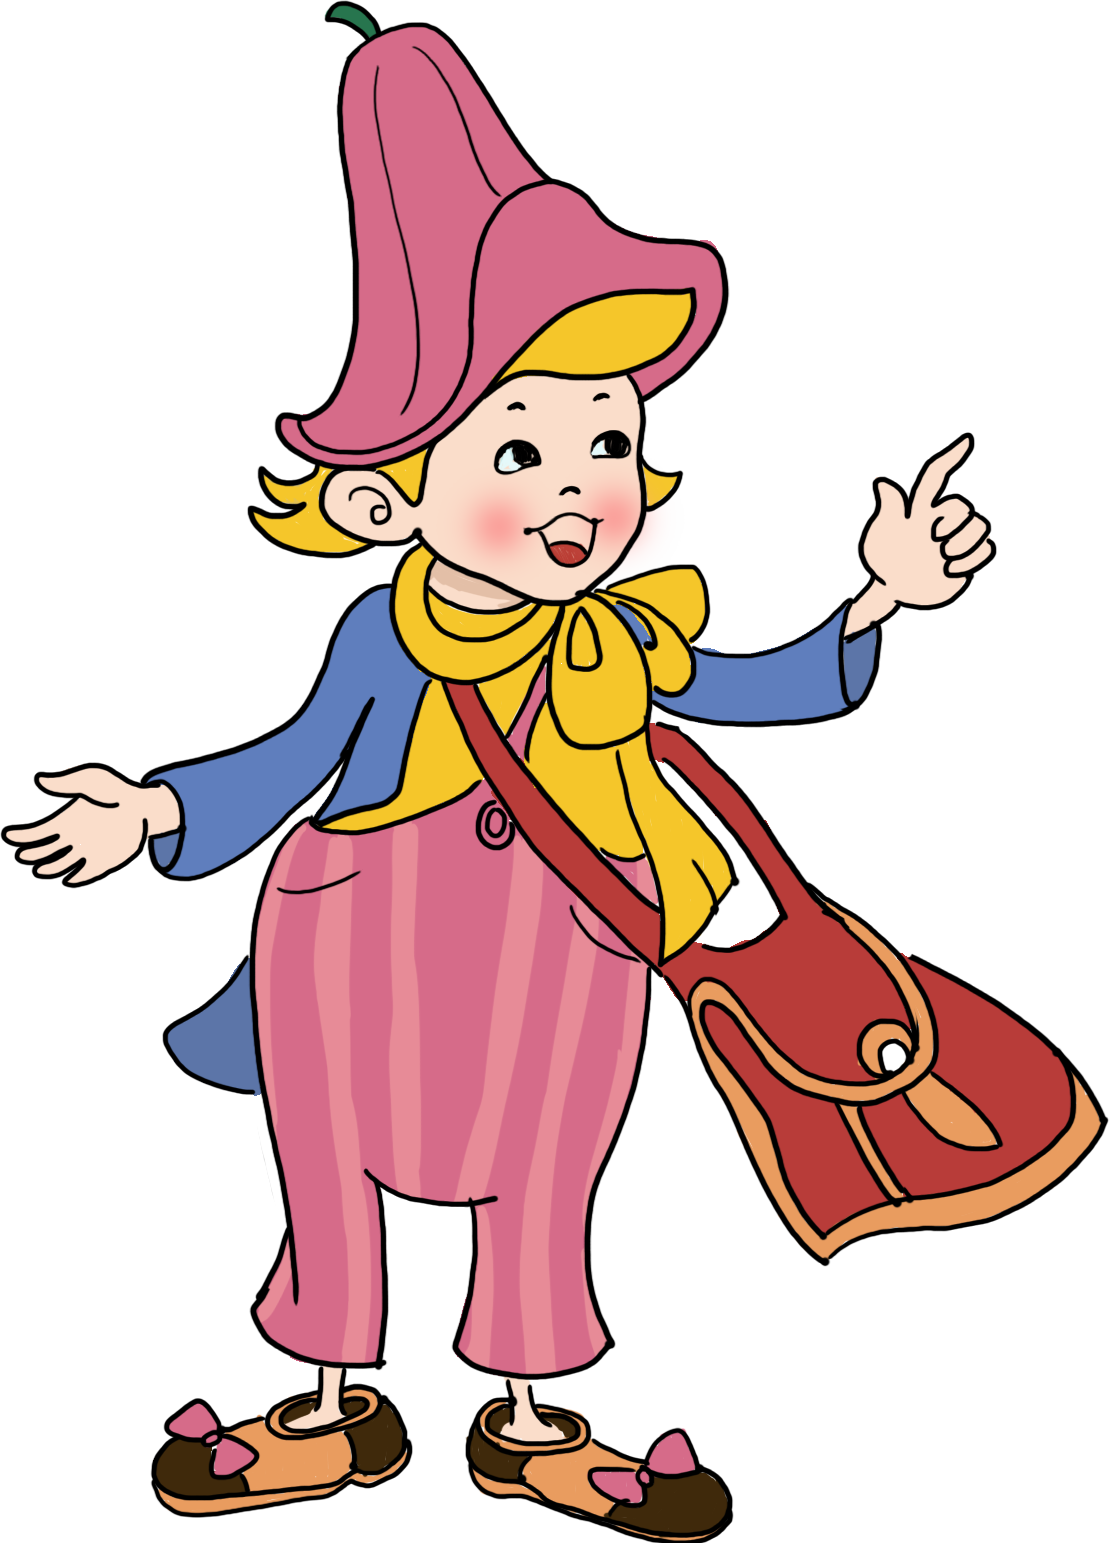
\includegraphics[width=0.2\linewidth]{Hinh0_HoaGiay}
		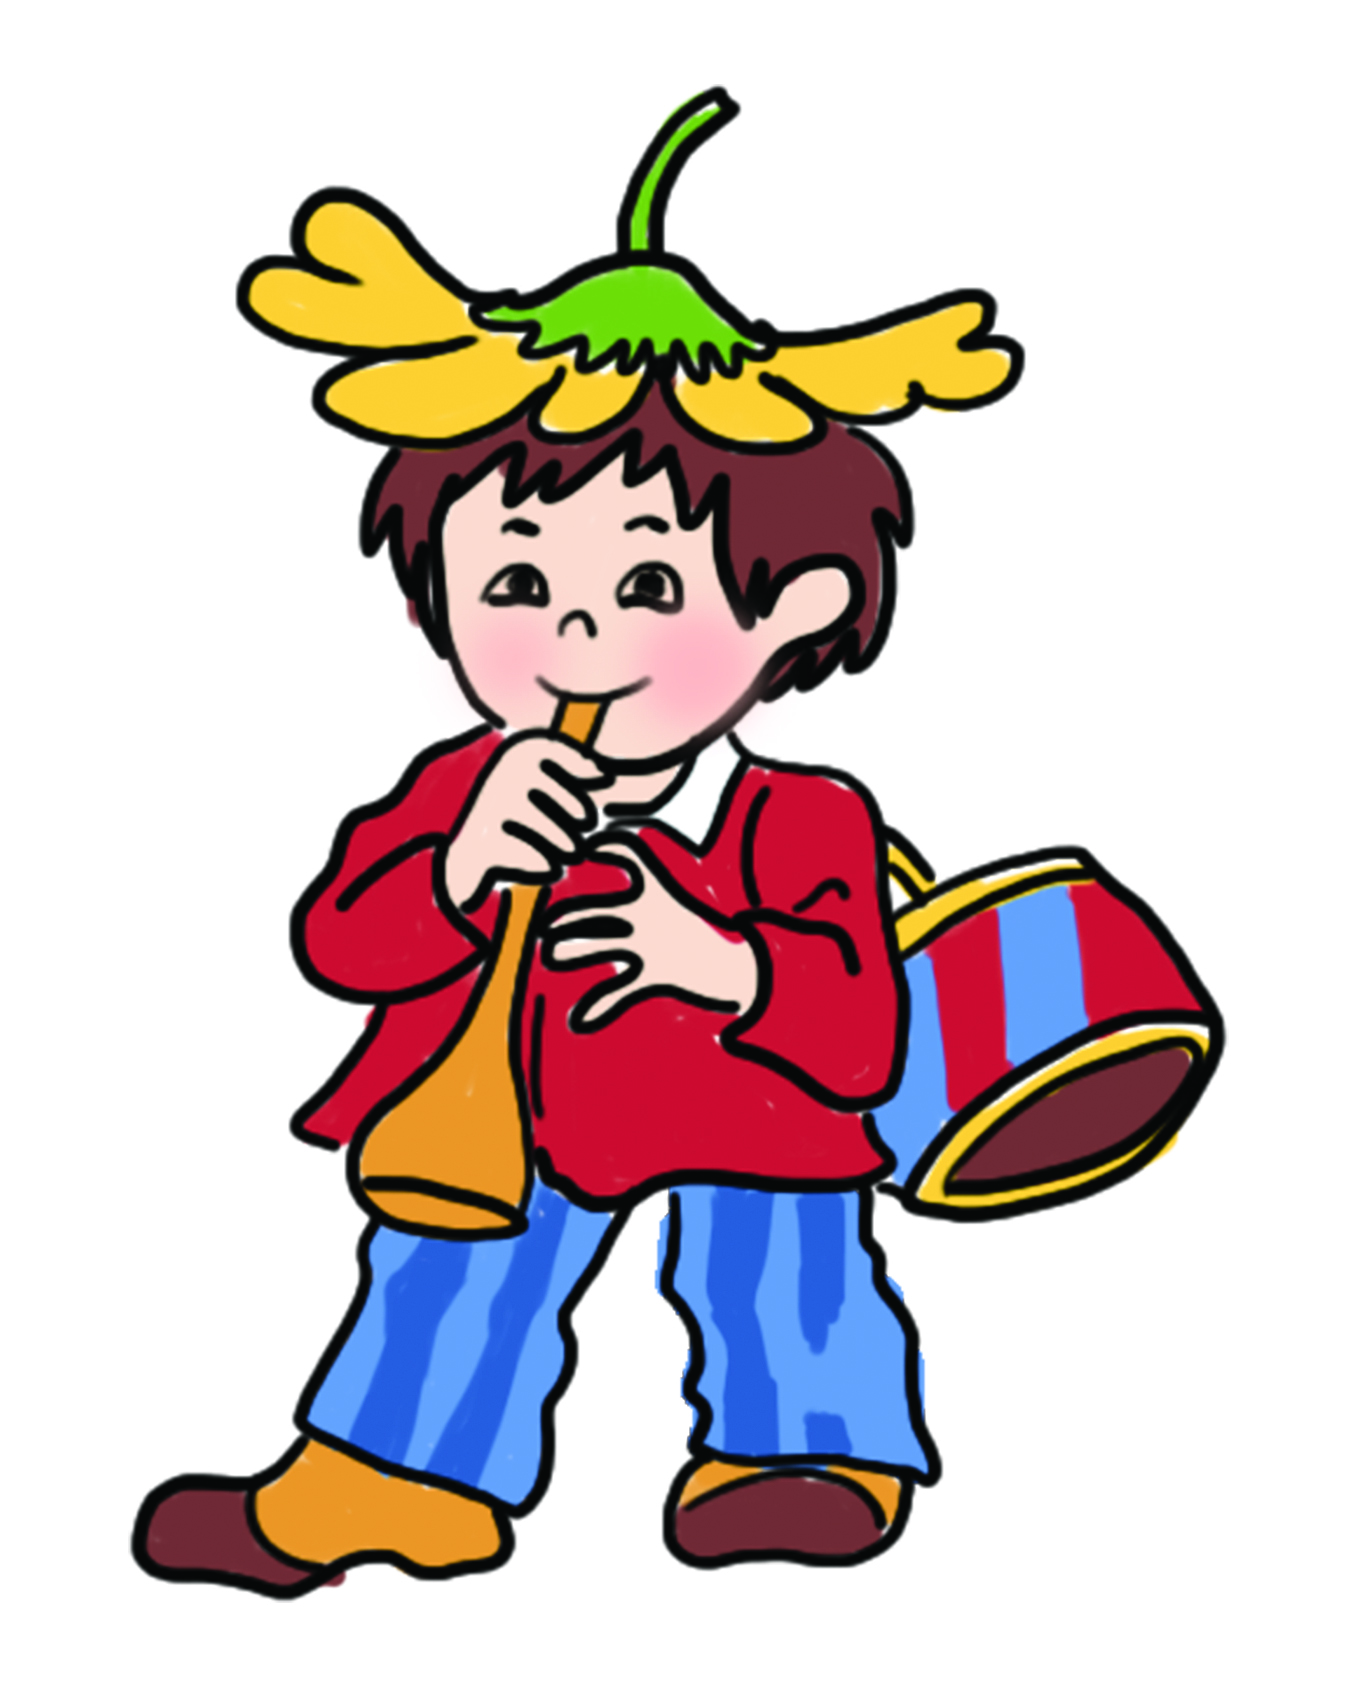
\includegraphics[width=0.2\linewidth]{Hinh0_KenDong}
		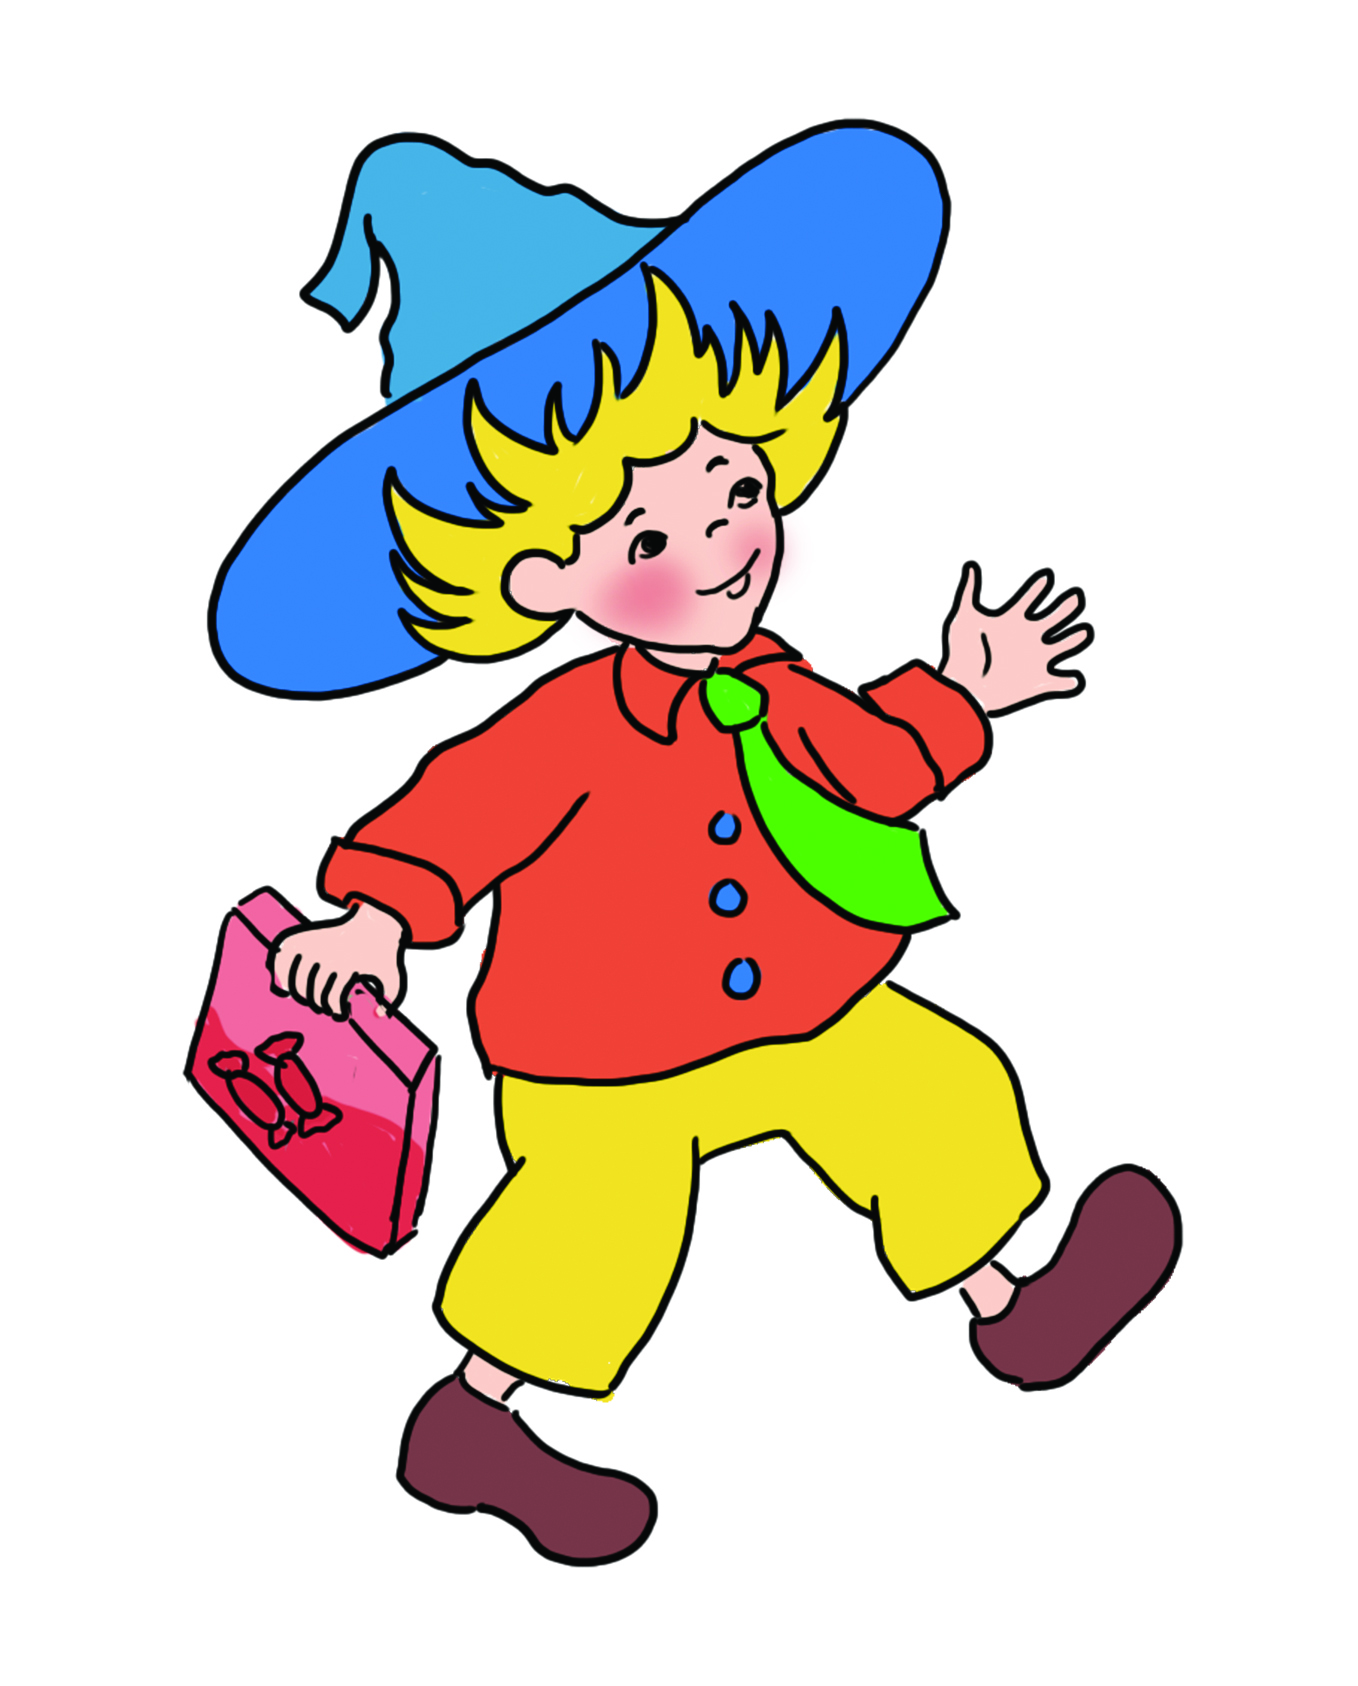
\includegraphics[width=0.2\linewidth]{Hinh0_MitDac}
		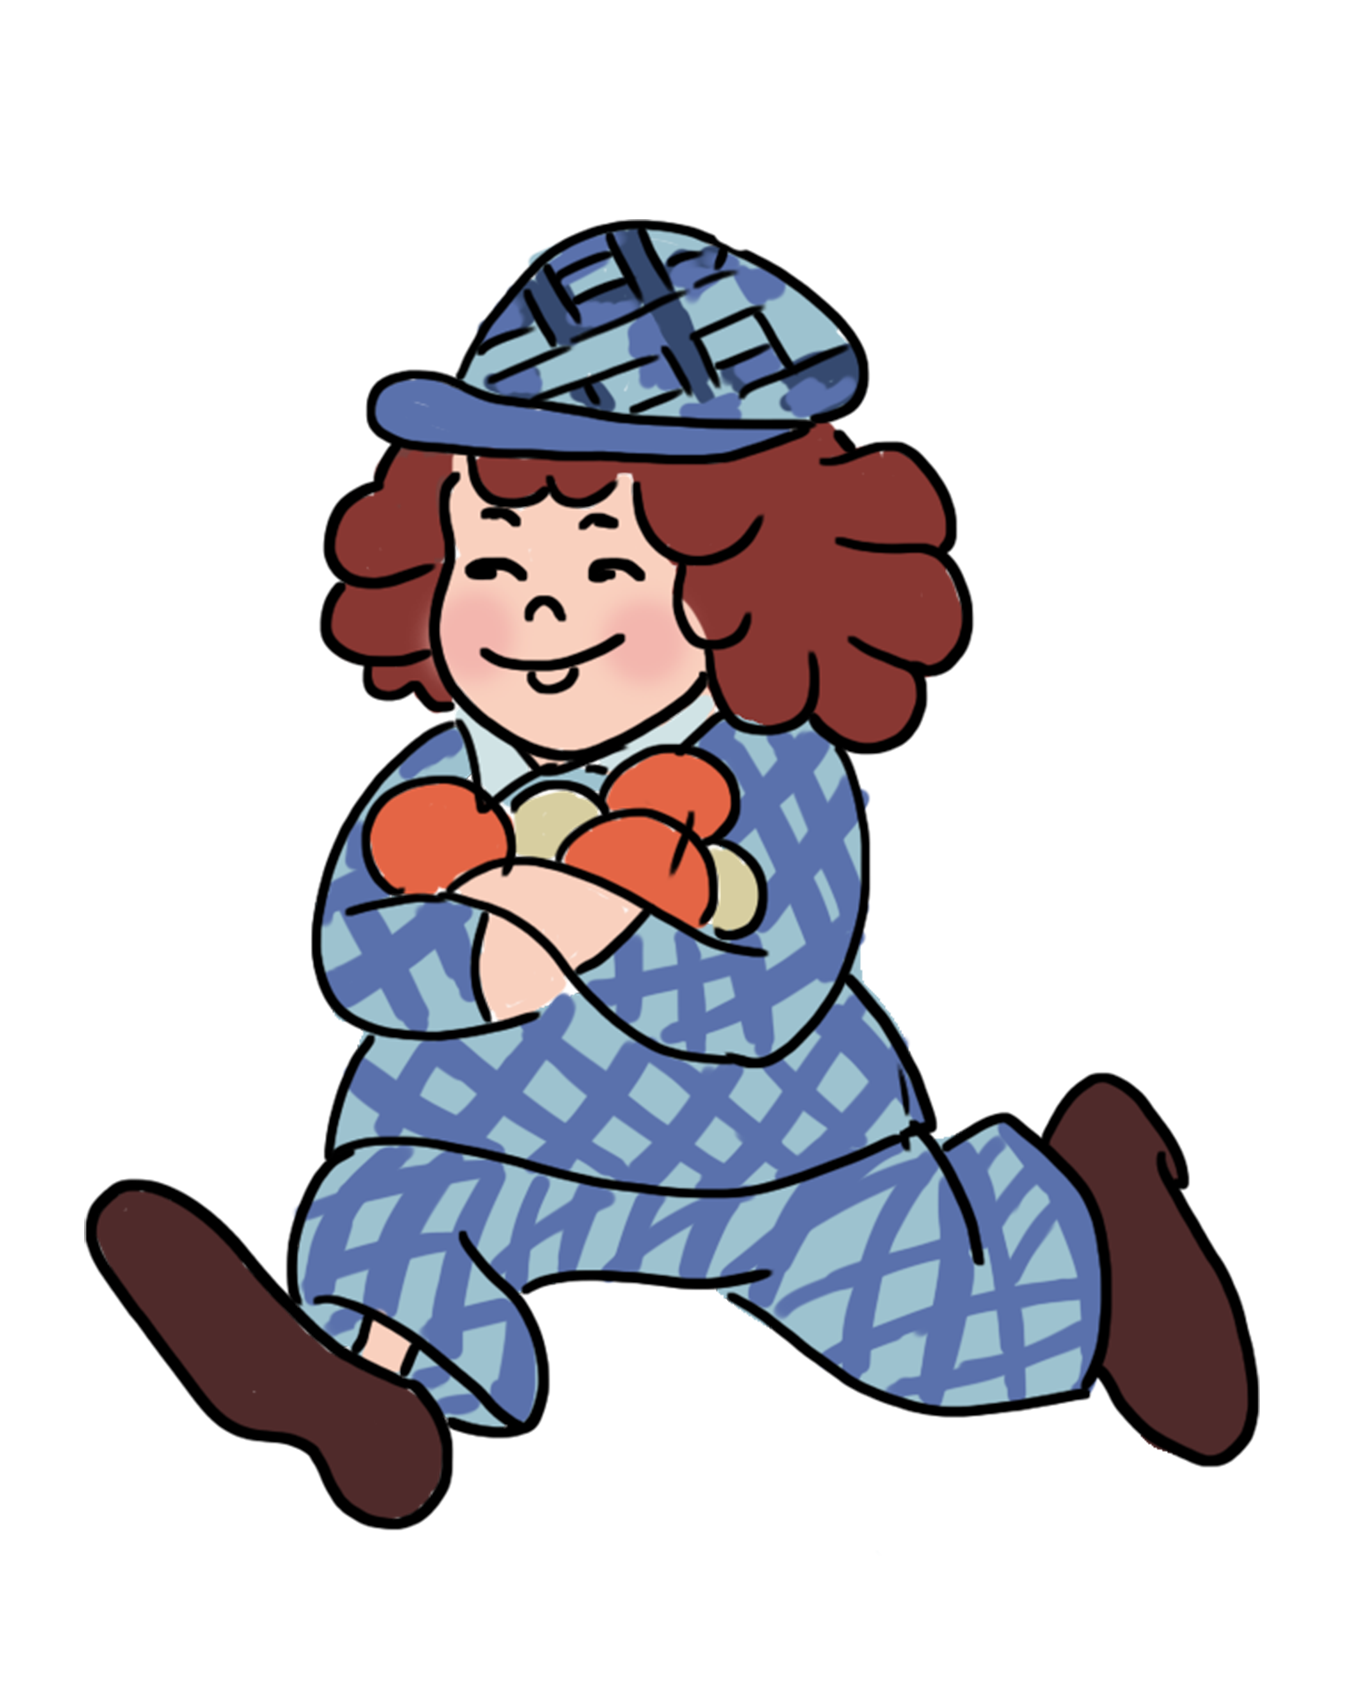
\includegraphics[width=0.2\linewidth]{Hinh0_NuocDuong}
		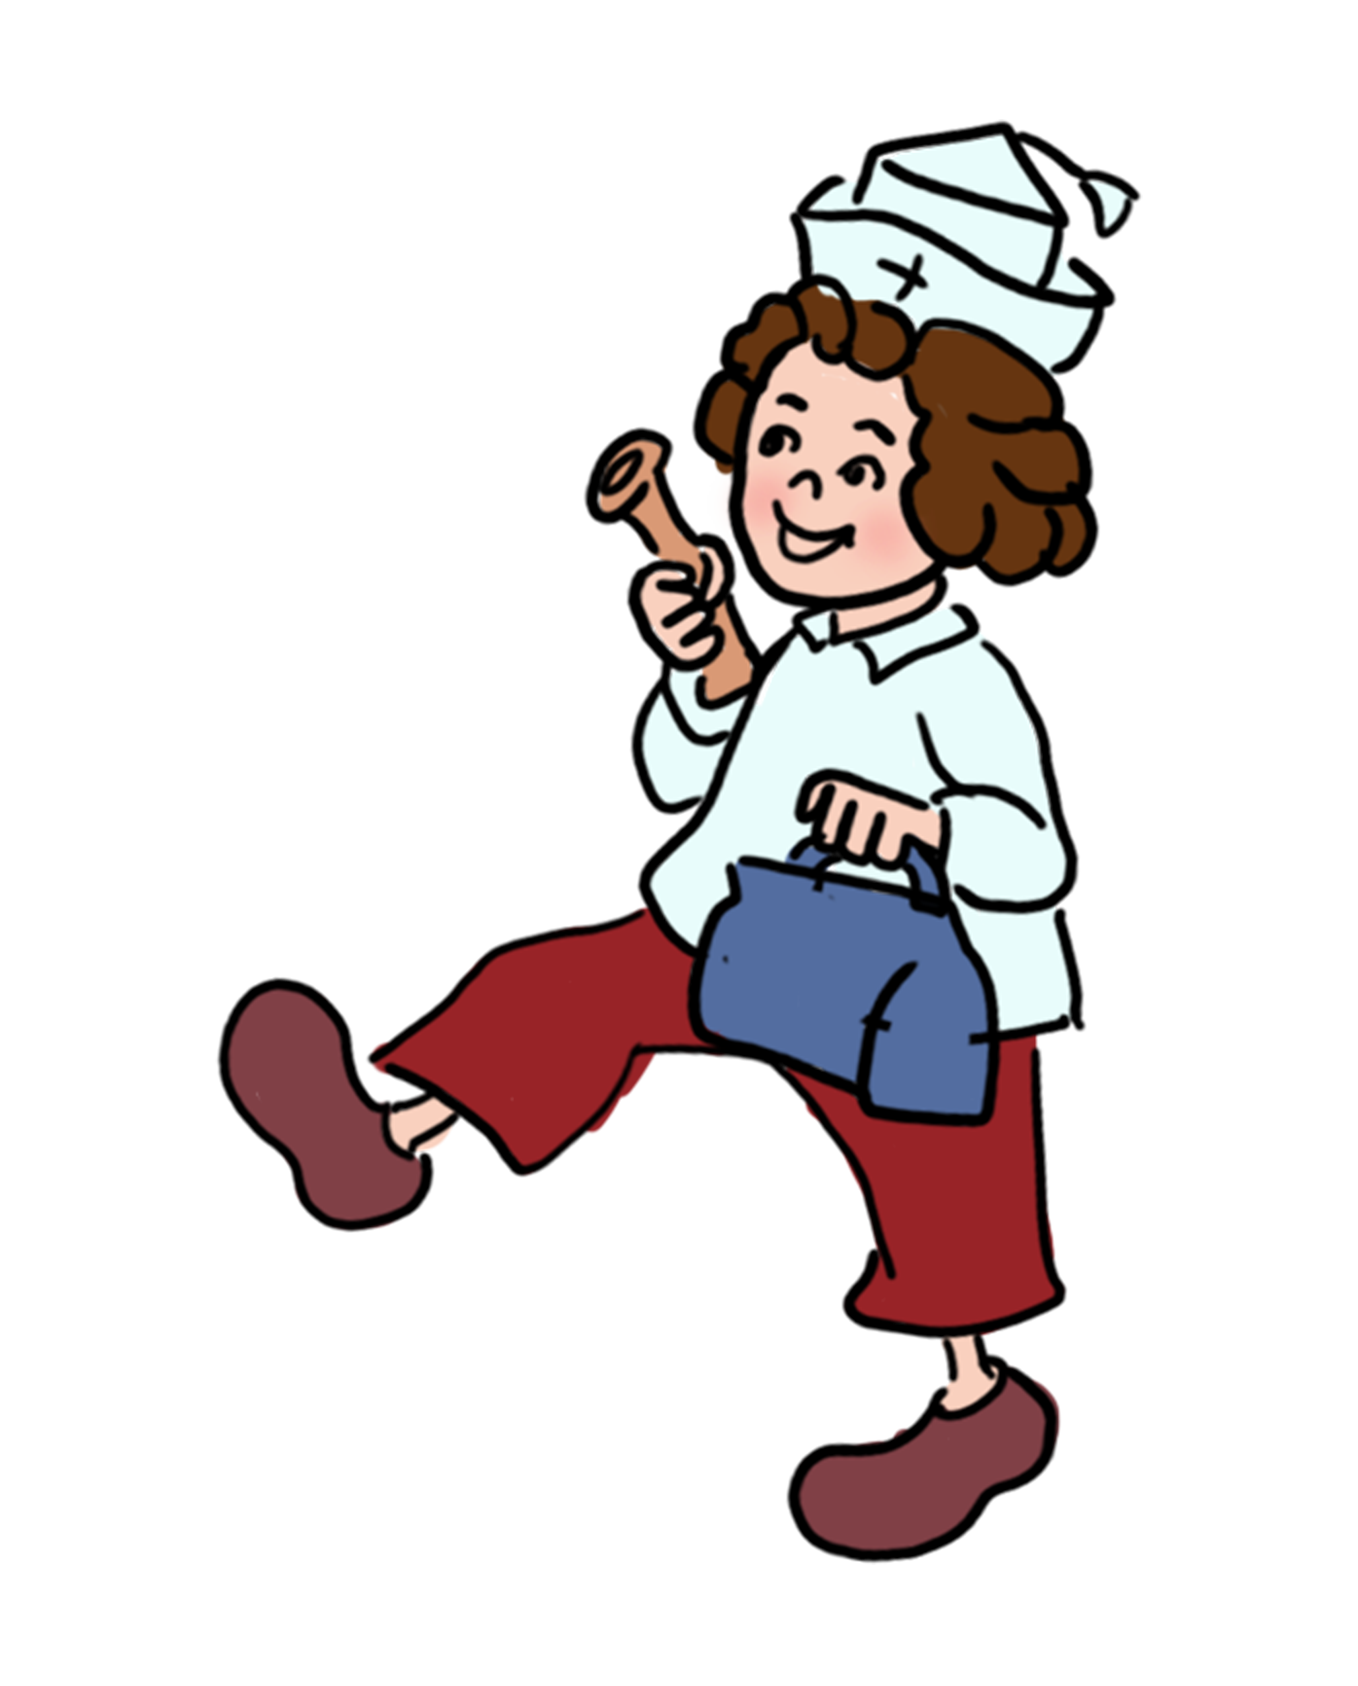
\includegraphics[width=0.2\linewidth]{Hinh0_ThuocVien}
		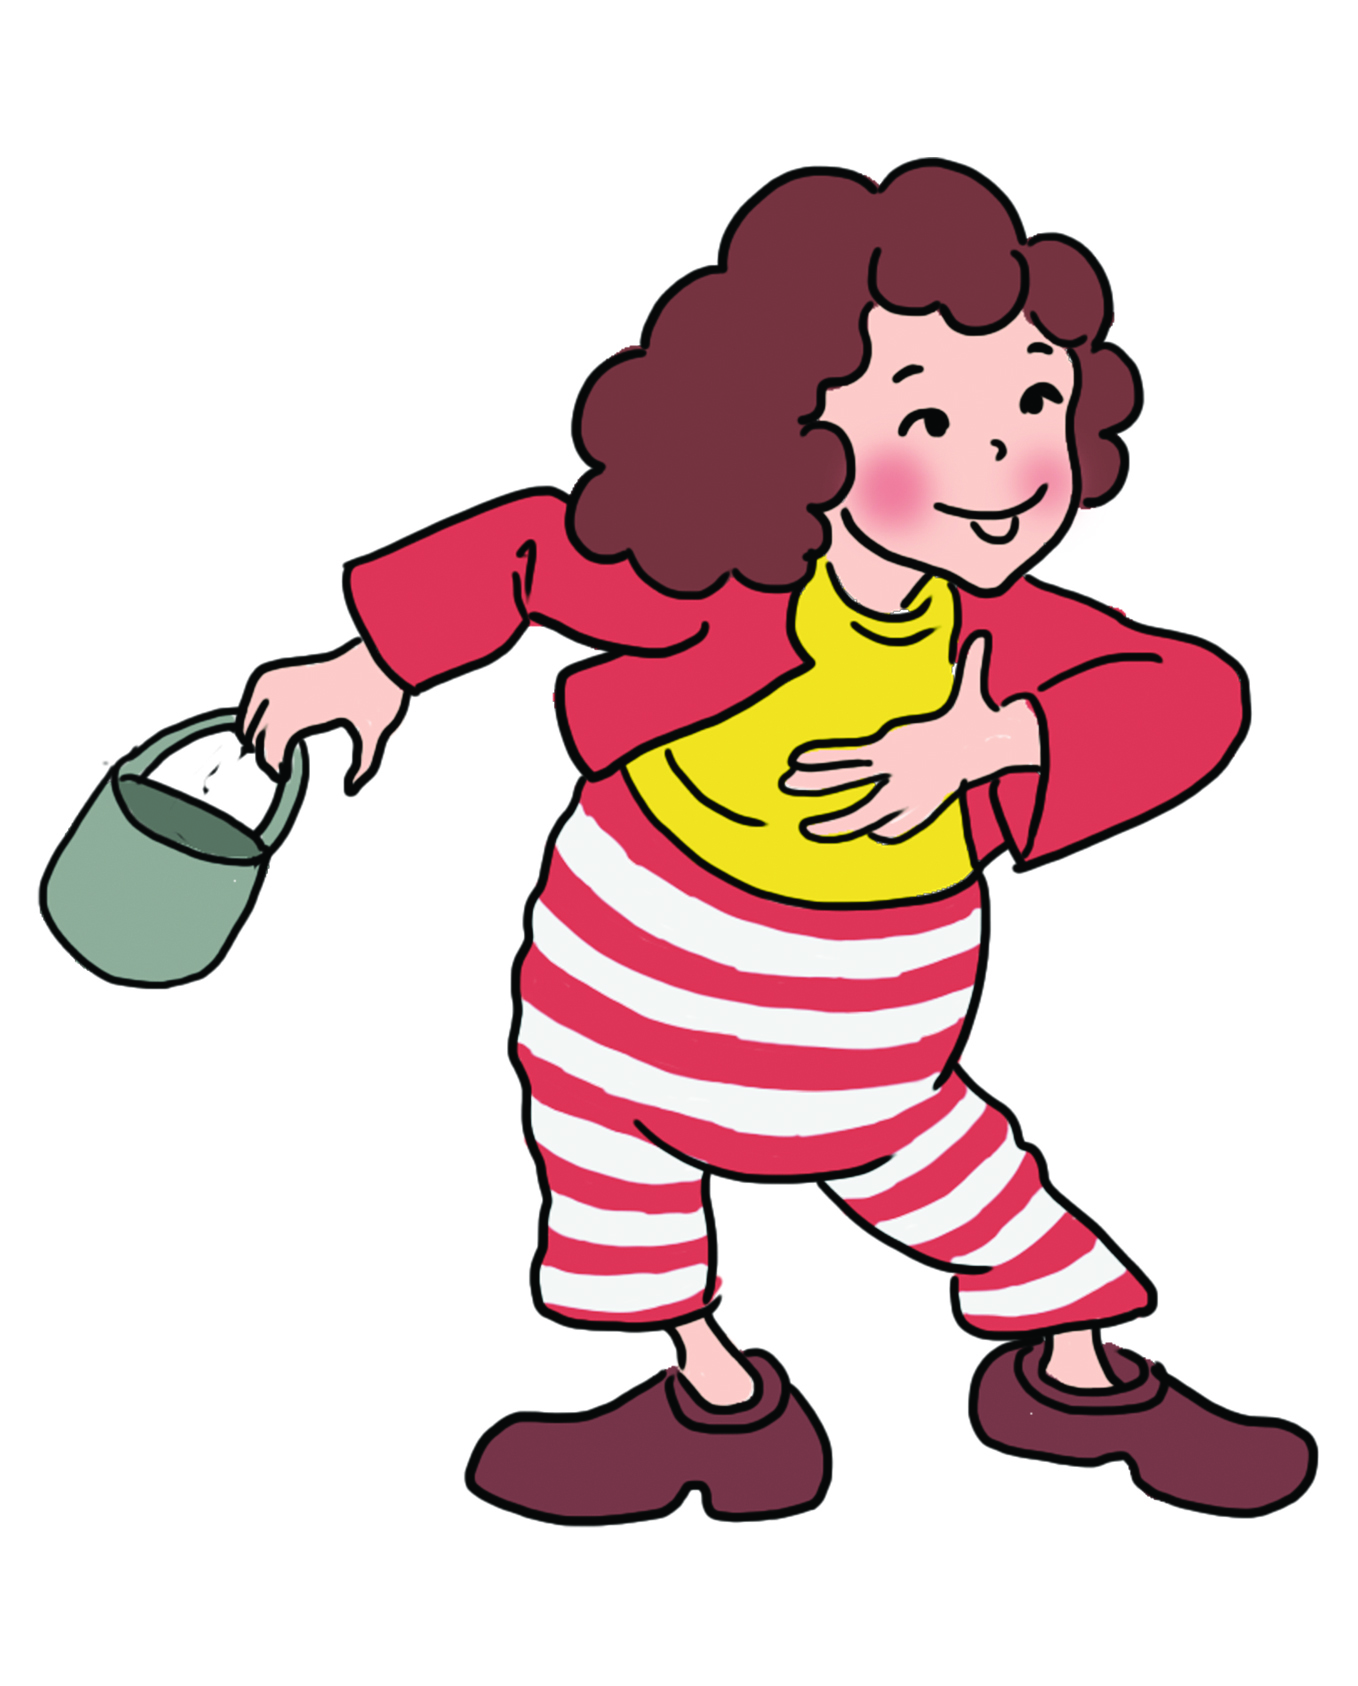
\includegraphics[width=0.2\linewidth]{Hinh0_VienDan}
		%\caption{\textit{\color{toancuabi}Hình $1$. Thành phố Hoa}}
		\vspace*{-10pt}
	\end{figure}	
	Mặc dù học không thành công, nhưng sau những lần theo học, Mít Đặc cũng khá lên nhiều, và tinh thần ham học hỏi của chú được mọi người ghi nhận phần nào.
	\vskip 0.1cm
	\begin{wrapfigure}{r}{0.55\linewidth}
		\centering
		\vspace*{-15pt}
		\captionsetup{labelformat= empty, justification=centering}
		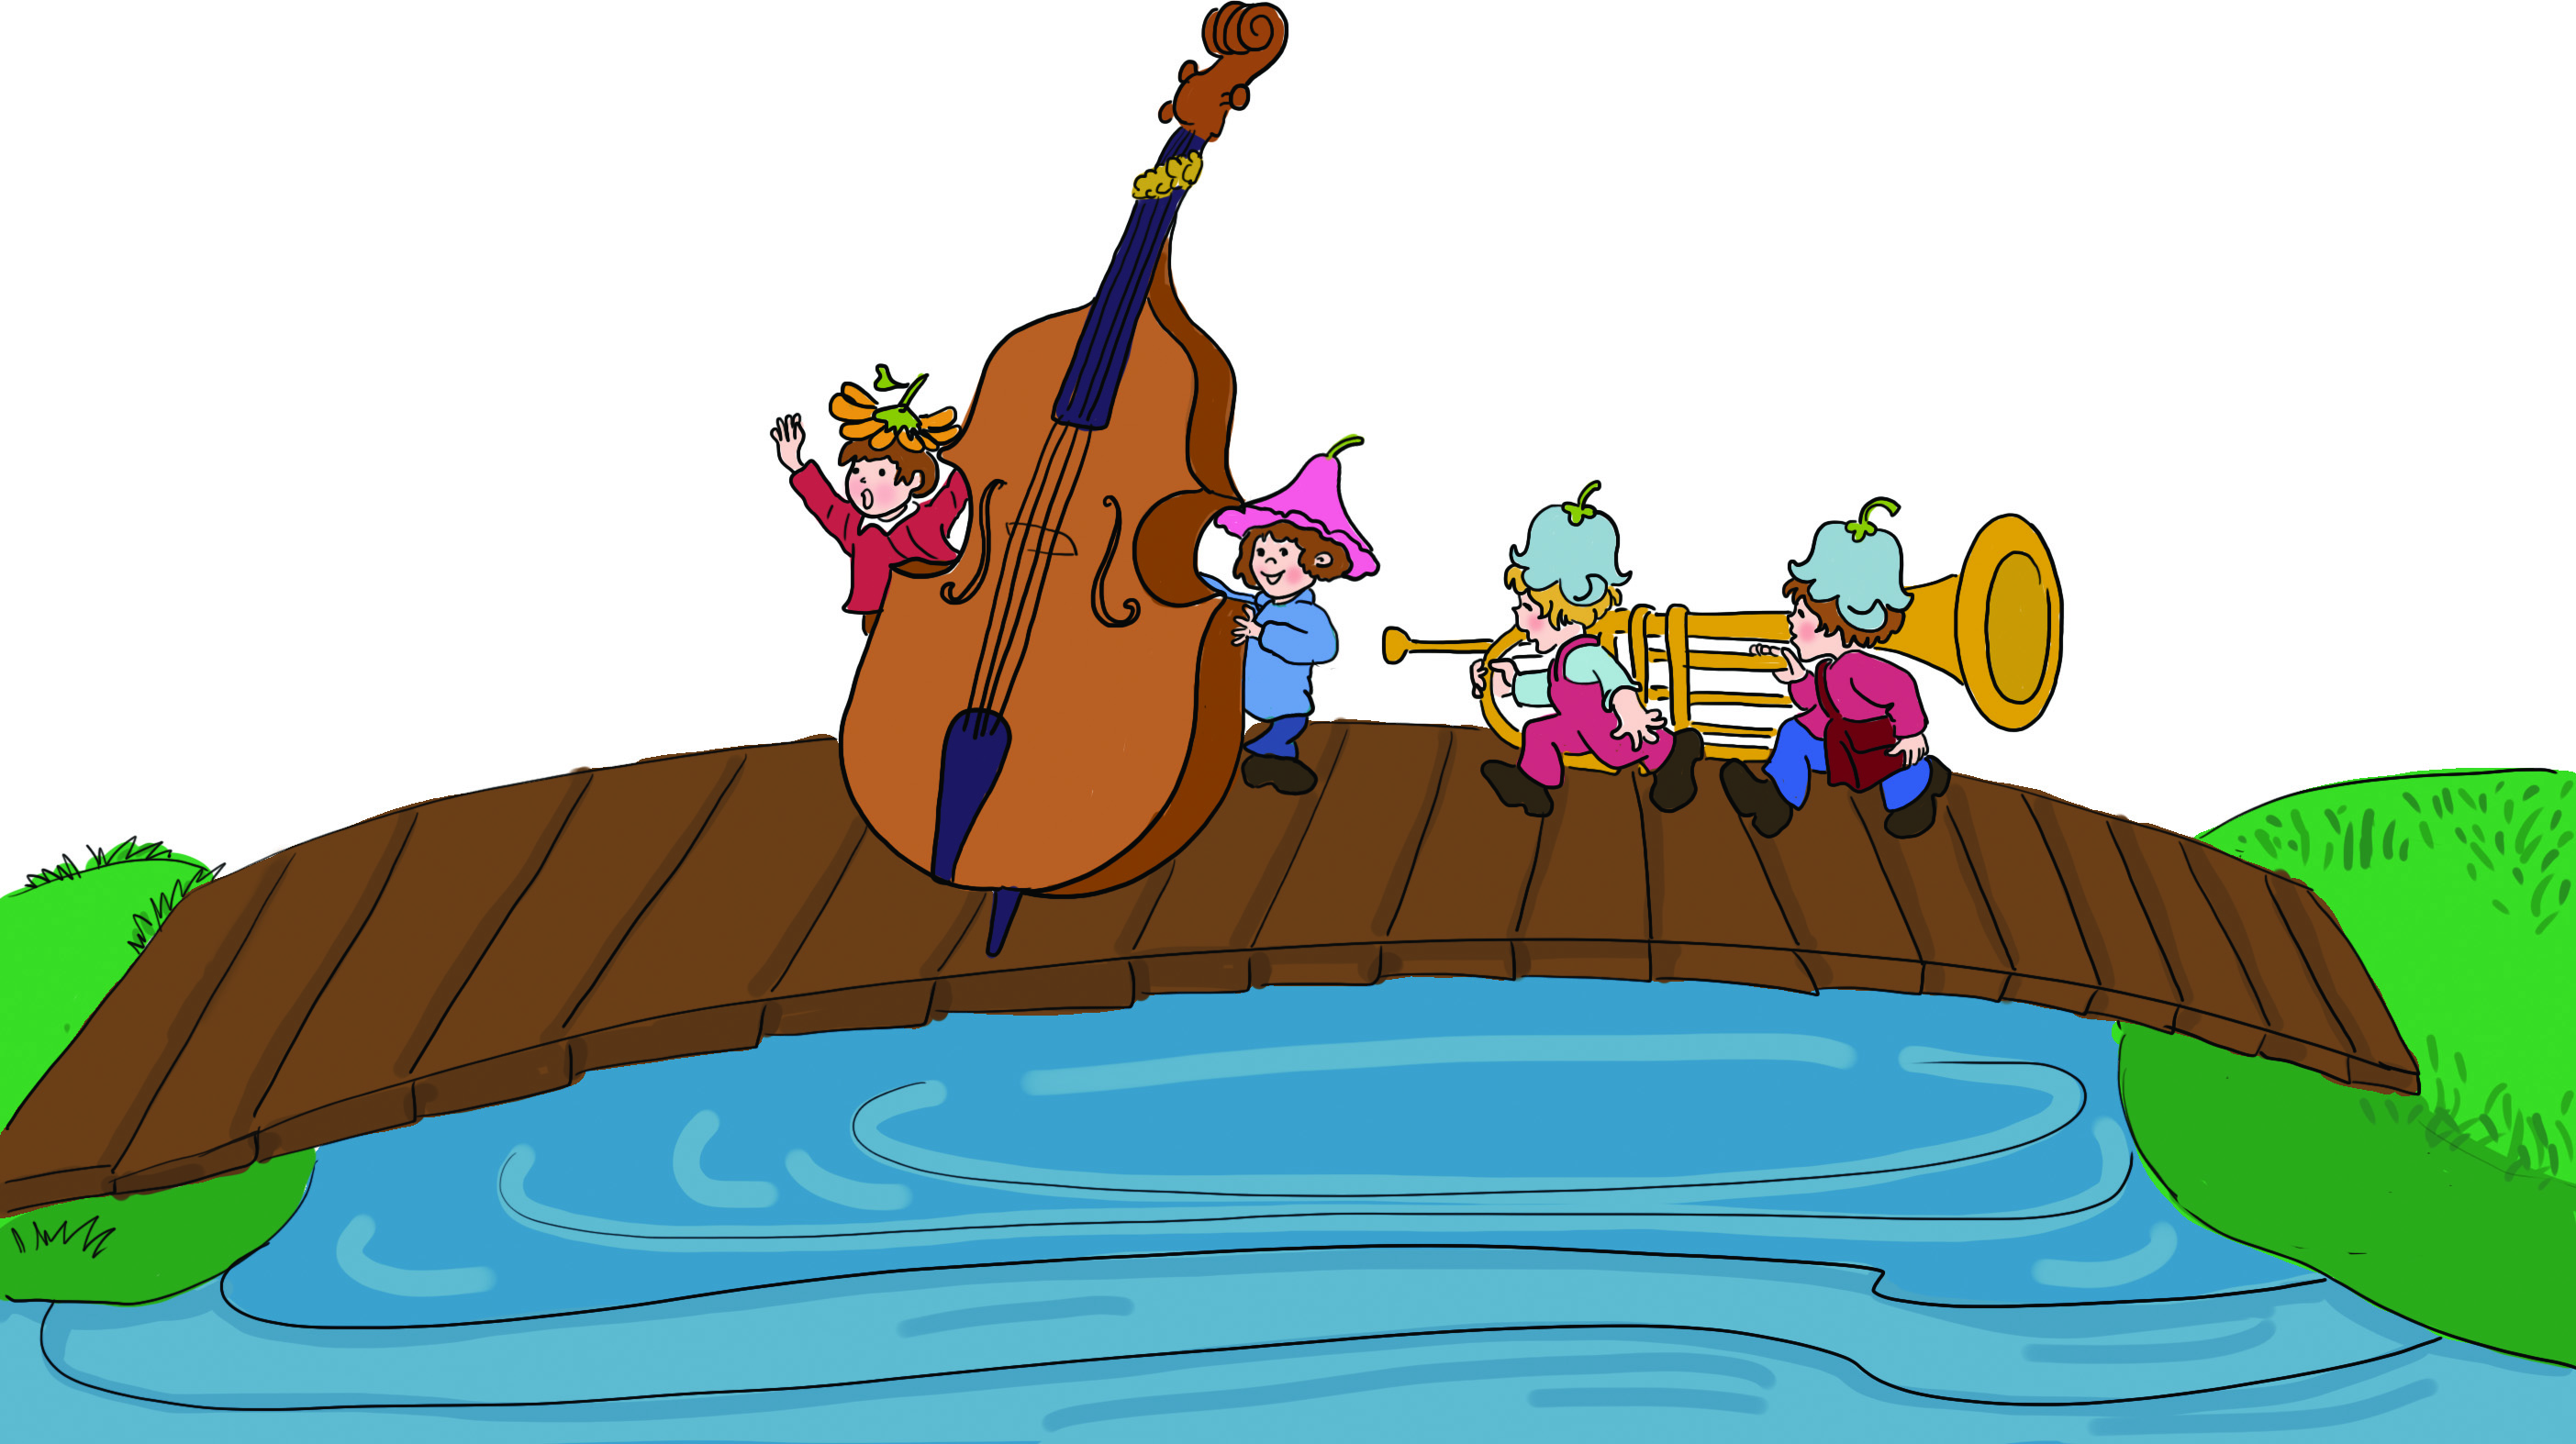
\includegraphics[width=1\linewidth]{Hinh3_KhiengNhacCu}
		%\caption{\textit{\color{toancuabi}Hình $3$.}}
		\vspace*{-20pt}
	\end{wrapfigure}
	\textbf{\color{toancuabi}Câu chuyện $\pmb{1.}$} Mặc dù kết quả học nhạc của Mít Đặc không được như ý, nhưng Kèn Đồng vẫn ghi nhận những cố gắng của cậu. Một lần, Kèn Đồng được mời đi biểu diễn và đã rủ cả Mít Đặc, Biết tuốt và Nhanh Nhảu cùng đi. Bốn chú đã đi bộ tới một buổi biểu diễn vào ban đêm. Họ quyết định đi tắt, nhưng vì thế phải đi qua một chiếc cầu gỗ khá chênh vênh qua dòng sông Dưa Chuột. Thật là may, họ có một chiếc đèn pin. Do các nhạc cụ của họ có kích thước khác nhau, nên mỗi người cần một khoảng thời gian khác nhau để đi qua được chiếc cầu. Nhanh Nhảu cần $1$ phút, Kèn Đồng cần $2$ phút, Biết Tuốt cần $5$ phút và Mít Đặc cần tận $10$ phút. Họ cần phải đi qua cầu theo từng cặp với vận tốc chậm nhất, ví dụ như nếu người đi $1$ phút đi cùng với người đi $10$ phút, thì cần phải mất đúng $10$ phút mới qua cầu. Do họ chỉ có một chiếc đèn pin, nên một người phải quay lại đầu cầu bên kia, và sau đó một cặp khác lại đi sang tiếp. Các chú chỉ có đúng $17$ phút để đi vượt qua cầu để tới buổi trình diễn đúng giờ. Các chú sẽ phải đi qua cầu theo thứ tự nào để tất cả $4$ người đều vượt qua được cầu và tới buổi hòa nhạc đây? Chắc là Biết Tuốt phải ra tay rồi. Các bạn tính cùng Biết Tuốt nhé.
	\vskip 0.1cm
	\textbf{\color{toancuabi}Câu chuyện $\pmb{2.}$} Từ ngày theo thi sĩ Hoa Giấy làm thơ, đi đâu Mít Đặc cũng ứng khẩu thành thơ. Một lần nọ, đi ra chợ, thấy Nước Đường đang mang cam và táo để đổi lấy lê của cô tí hon Hoa Cúc, Mít Đặc liền ứng khẩu ngay.
	\vskip 0.1cm
	\begin{adjustwidth}{90pt}{0pt}
				\begin{flushleft}
					\textit{Năm cam đổi được sáu quả lê\\
			Kèm thêm bốn táo thật là phê\\
			Quả nào cũng ngon cũng thơm ngọt\\
			Càng ăn càng khỏe khỏi bị chê.\\
			Nay đổi ba lê lấy bảy táo\\
			Người mê lê thấy thật là hời\\
			Nước Đường có mười cam cùng sáu táo\\
			Bao nhiêu lê đổi được Hoa Cúc ơi?}
				\end{flushleft}
	\end{adjustwidth}
	\vskip 0.1cm
	Lần này thì thơ của Mít Đặc được các bạn của cậu rất là hoan nghênh, nhưng khi Nước Đường hỏi mình đổi được bao nhiêu lê của Hoa Cúc thì Mít Đặc lại chịu. Các bạn giúp cậu ấy nhé.
	\begin{figure}[H]
		\centering
		\vspace*{-5pt}
		\captionsetup{labelformat= empty, justification=centering}
		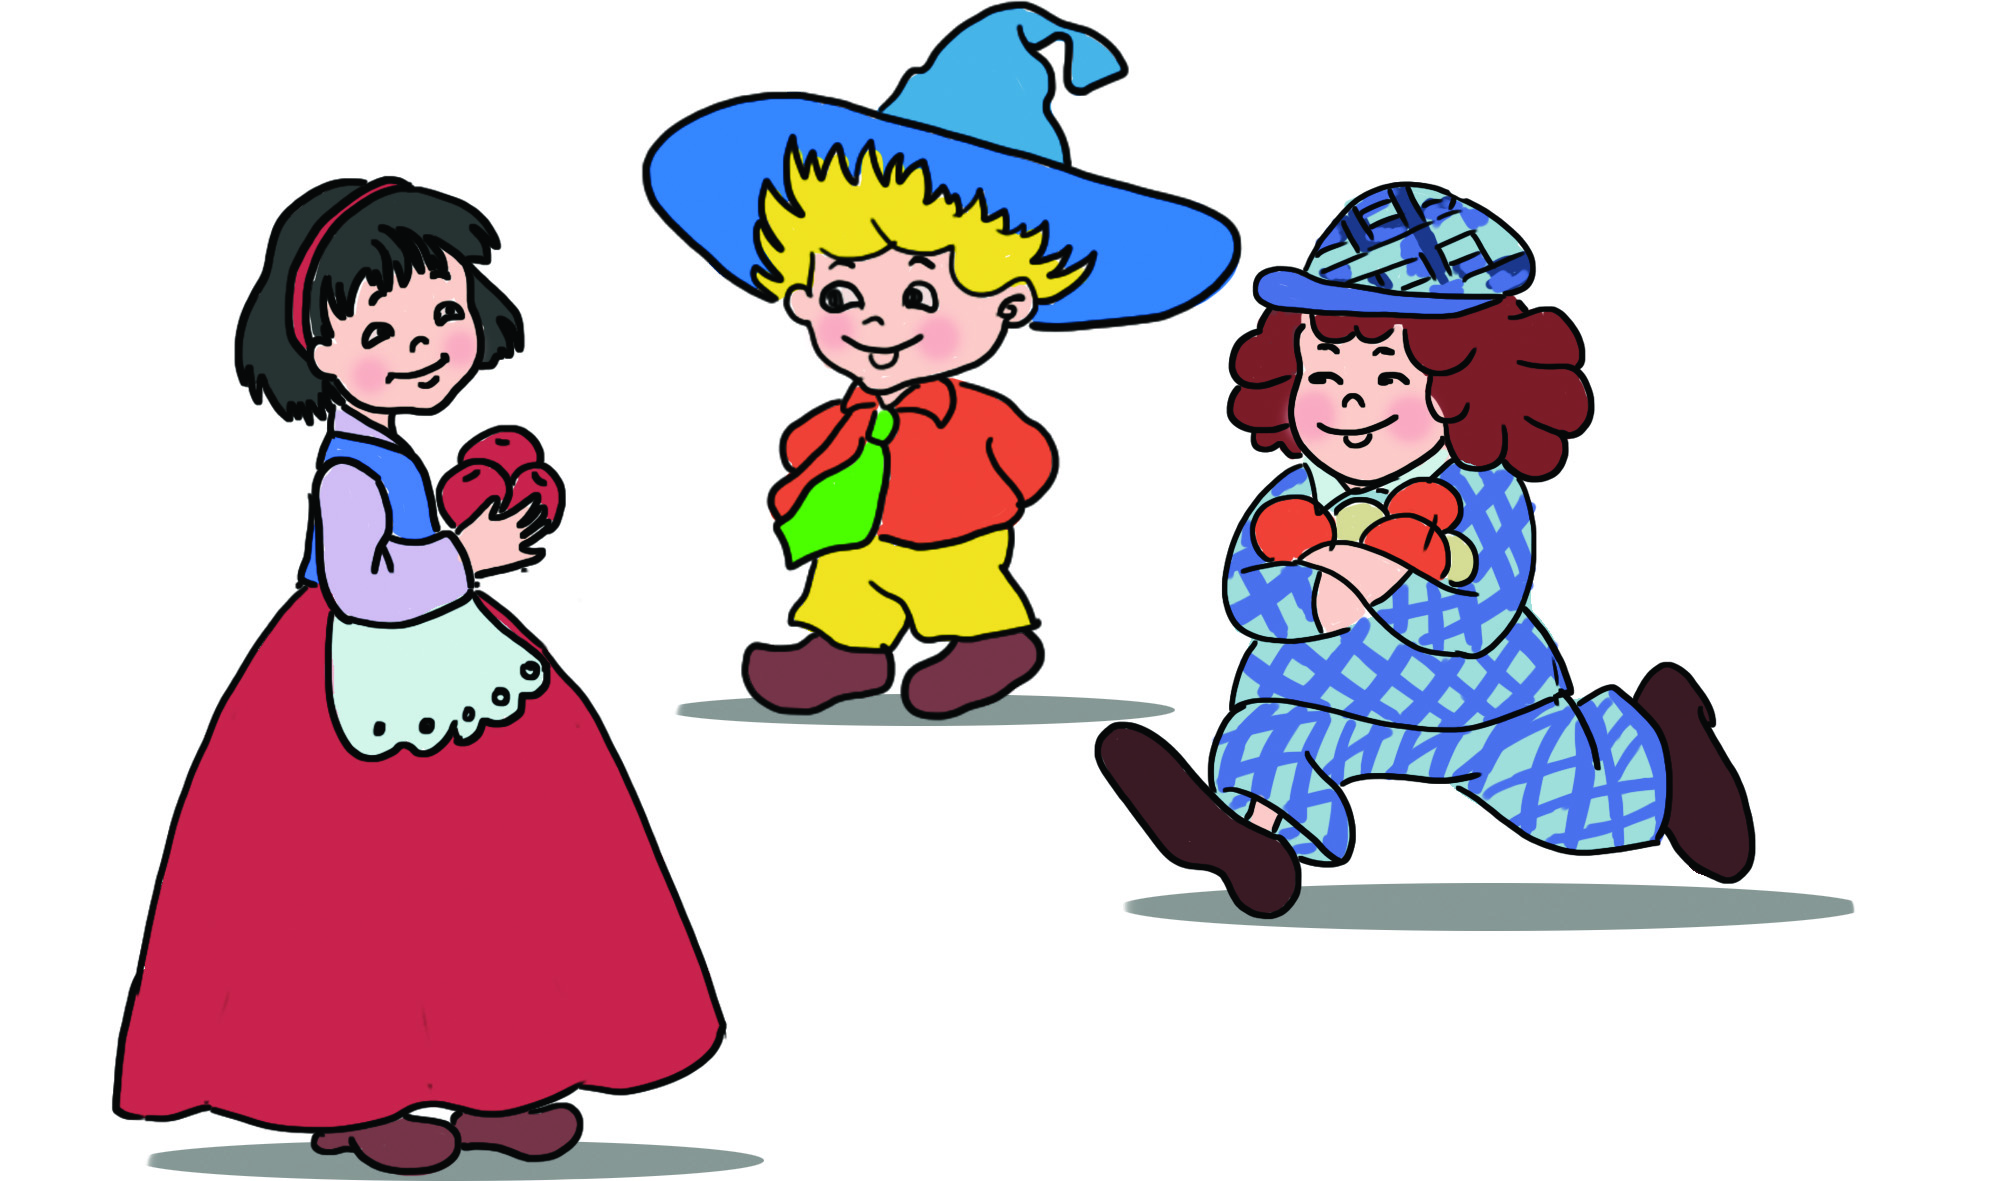
\includegraphics[width=0.6\linewidth]{Hinh4_TaoLe}
		%\caption{\textit{\color{toancuabi}Hình $4$.}}
		\vspace*{-10pt}
	\end{figure}
	\textbf{\color{toancuabi}Câu chuyện $\pmb{3.}$} Chú thợ máy Bu Loong và chú phụ lái Đinh Vít mới cải tiến được một loại ô tô mới, các chú tí hon ai cũng háo hức để được lái thử. Mít Đặc cũng thích lắm, nhưng sau vụ lái ô tô làm náo động cả phố thì e là Bu Loong không cho cậu lái nữa. Ở thành phố Hoa, các loại xe được chạy bằng nước ngọt có ga nén. Mít Đặc nghĩ ra một cách là mua nước ngọt để tặng cho Bu Loong và Đinh Vít để xin được lái chiếc xe này. Cậu mua được $6$ thùng nước ngọt (như hình vẽ) và những con số trên nắp thùng chính là thể tích nước ngọt bên trong. Mít Đặc chỉ giữ lại $1$ thùng, còn $5$ thùng đem tặng cho Bu Loong và Đinh Vít. Cậu tặng một số thùng cho Đinh Vít, một số thùng cho Bu Loong. Các bạn có biết Mít Đặc giữ lại thùng nào cho mình không, biết rằng Bu Loong nhận được lượng nước ngọt gấp đôi của Đinh Vít?
		\begin{figure}[H]
		\centering
		\vspace*{-5pt}
		\captionsetup{labelformat= empty, justification=centering}
		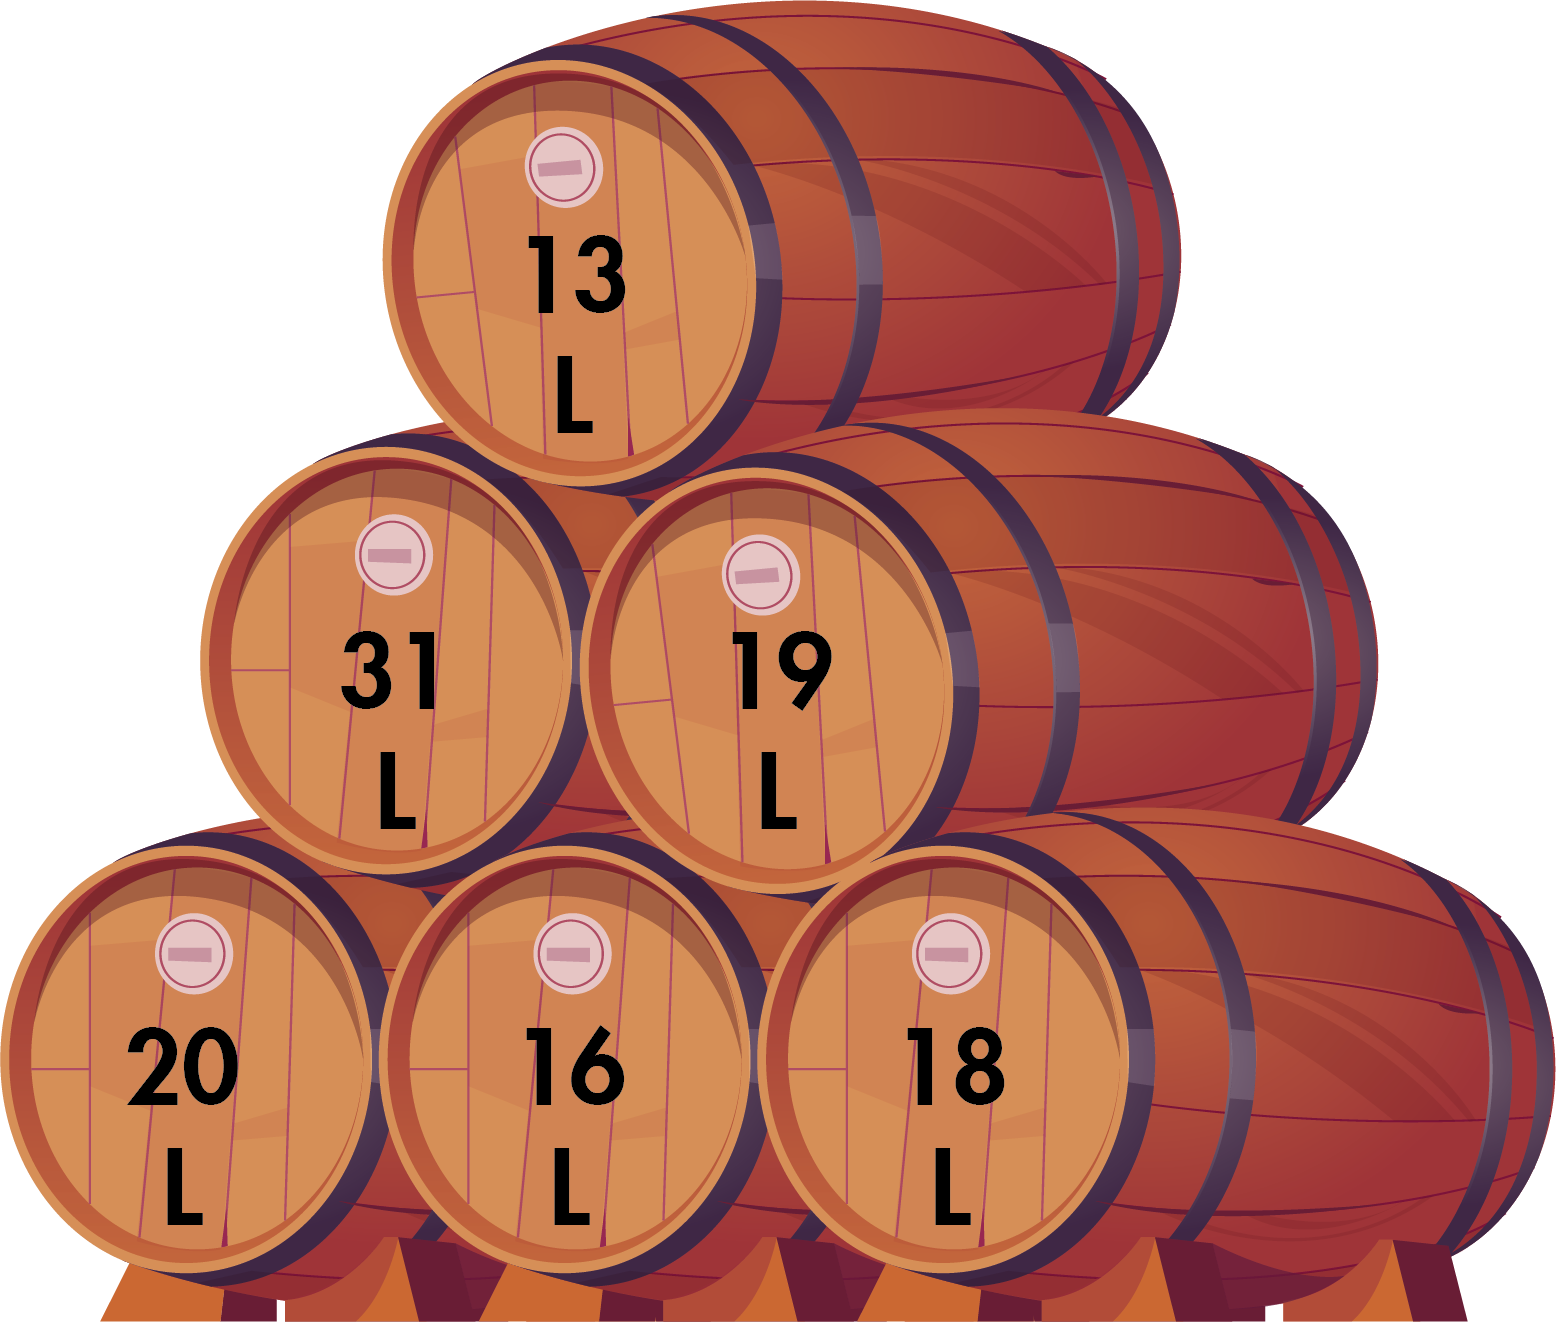
\includegraphics[width=0.4\linewidth]{Hinh5}
		%\caption{\textit{\color{toancuabi}Hình $5$.}}
		\vspace*{-10pt}
	\end{figure}
	\textbf{\color{toancuabi}Câu chuyện $\pmb{4.}$} Nhân dịp kỳ nghỉ kéo dài, Mít Đặc muốn học vẽ lại nên đến năn nỉ Thuốc Nước dạy mình. Rút kinh nghiệm từ lần trước, lần này Thuốc Nước quyết sẽ thử thách “học trò” trước đã. Cậu đưa ra một lưới ô vuông $4\times 4$ như hình bên và bảo Mít Đặc hãy tô màu cho các ô vuông nhỏ, khi nào hoàn thành thì sẽ dạy cậu ấy vẽ tiếp.
	\begin{figure}[H]
		\centering
		\vspace*{-5pt}
		\captionsetup{labelformat= empty, justification=centering}
		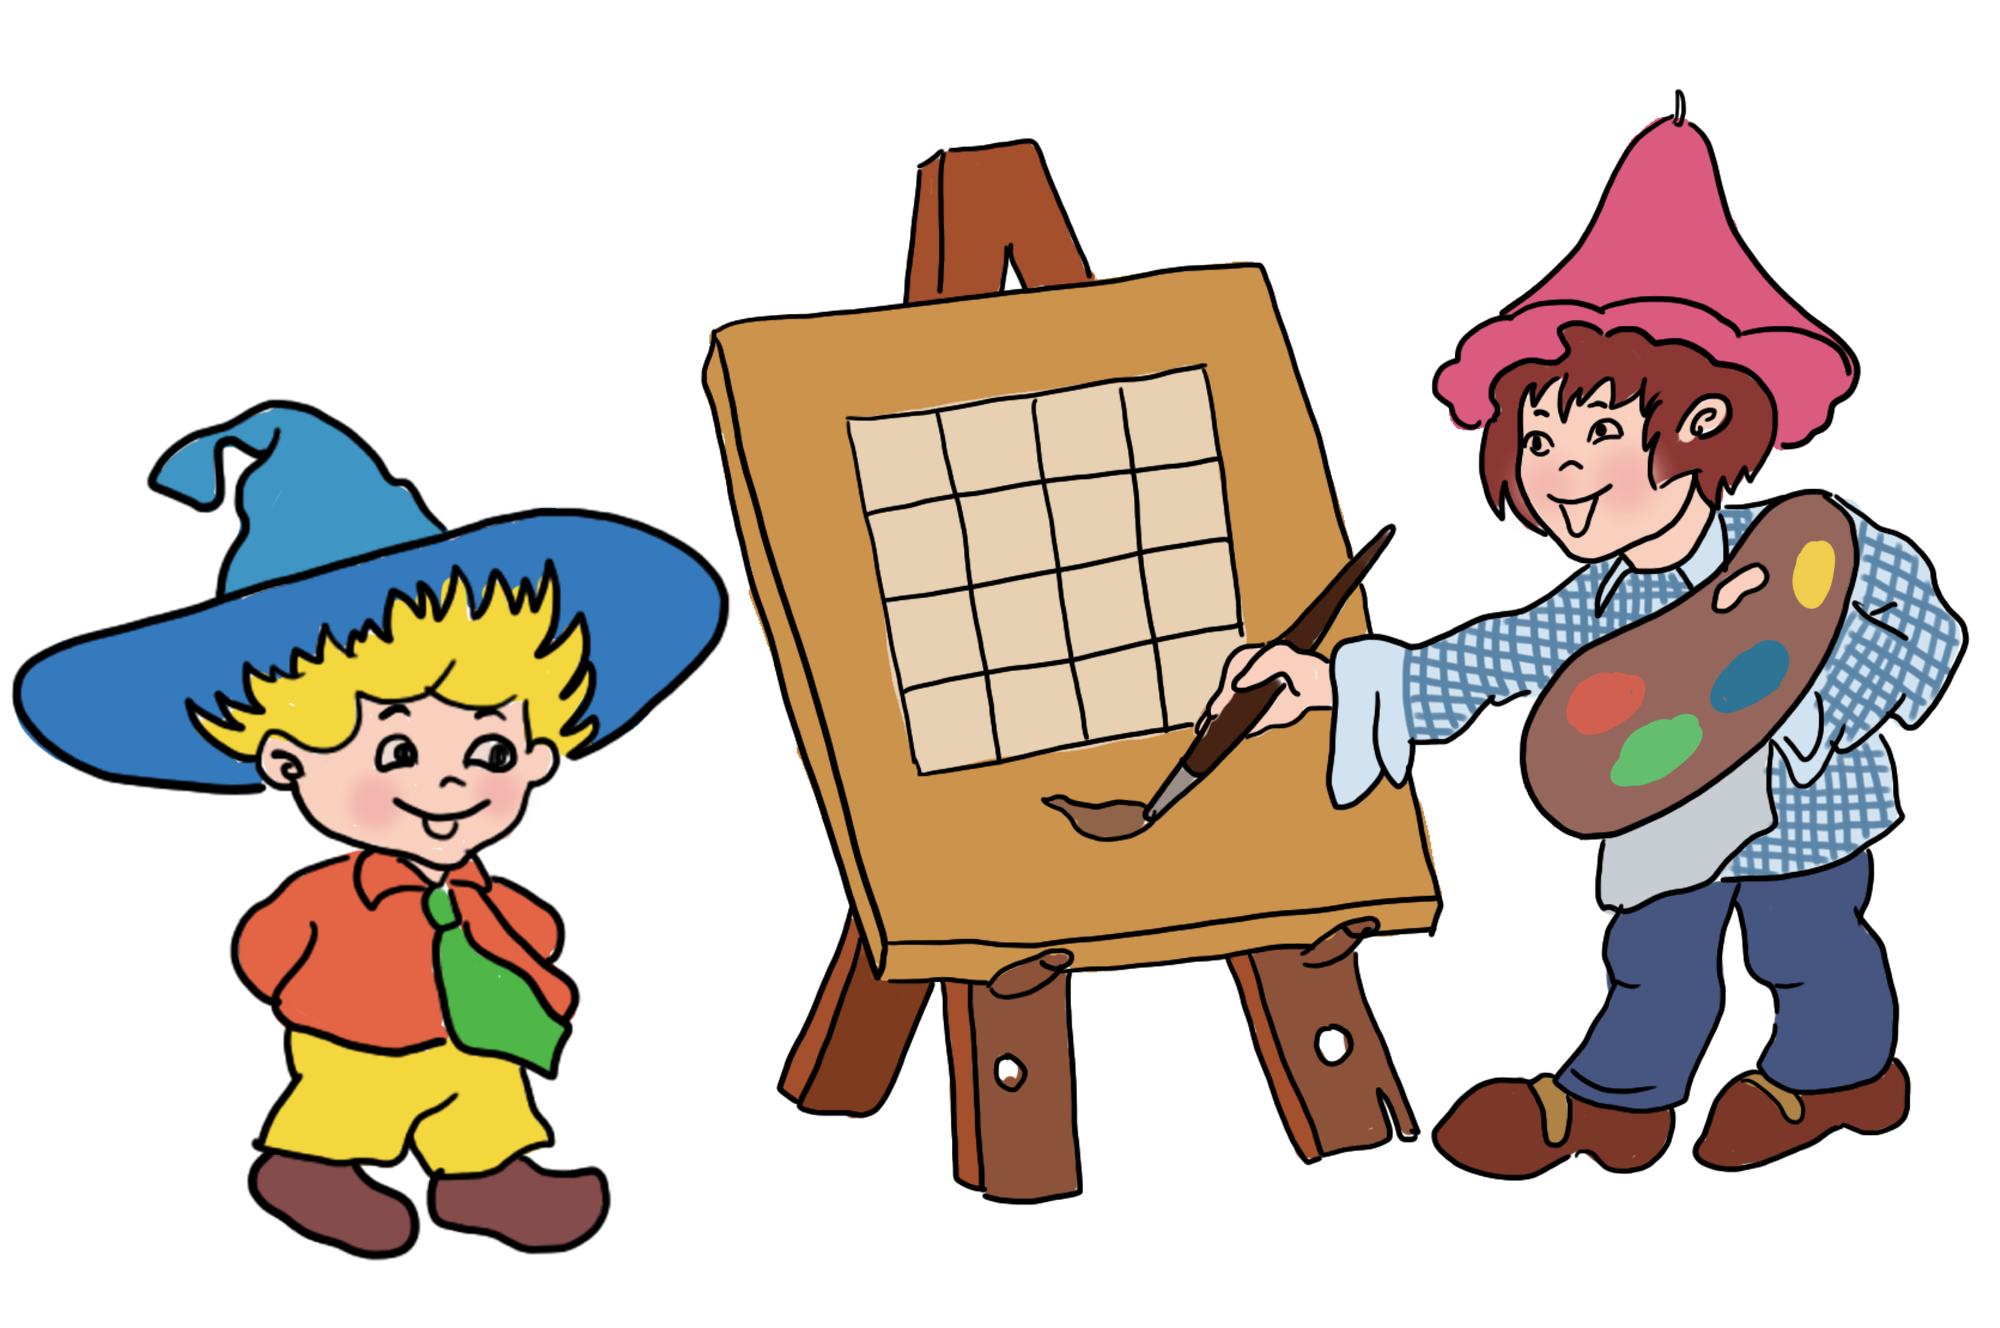
\includegraphics[width=0.6\linewidth]{Hinh6_Mit_dac_Thuoc_nuoc}
		%\caption{\textit{\color{toancuabi}Hình $6$.}}
		\vspace*{-10pt}
	\end{figure}
	Quy tắc tô màu lưới ô vuông mà Thuốc Nước đề ra là:
	\vskip 0.1cm
	-- Có $4$ ô vuông được tô màu xanh;
	\vskip 0.1cm
	-- Có $3$ ô vuông được tô màu đỏ;
	\vskip 0.1cm
	-- Có $3$ ô vuông được tô màu vàng;
	\vskip 0.1cm
	-- Có $3$ ô vuông được tô màu vàng tím;
	\vskip 0.1cm
	-- Có $3$ ô được tô màu nâu;
	\vskip 0.1cm
	-- Không có hai ô nào có cùng màu trên tất cả các hàng ngang,
	hàng dọc và đường chéo của lưới vuông.
	\vskip 0.1cm
	Các bạn hãy cùng Mít Đặc hoàn thành nhiệm vụ tô màu này nhé.
	\begin{center}
		\begin{tikzpicture}
			\draw[timhieukhoahoc,thick] (0,0) grid (4,4);
		\end{tikzpicture}
	\end{center}
	\centerline{\textbf{\color{toancuabi}Khám phá vùng đất mới bằng Kinh khí cầu}}
	\vskip 0.1cm
	\textit{Biết Tuốt thích đọc sách, cậu đã đọc rất nhiều sách kể chuyện những xứ sở xa xăm cũng như về các chuyến du lịch. Mỗi khi rỗi rãi, chú lại kể cho các bạn của mình nghe. Các chú tí hon rất thích nghe nói đến những đất nước kì lạ mà chưa từng được trông thấy bao giờ. Biết Tuốt kể cho các chú nghe nhiều đến nỗi các chú đâm ra mơ mộng, mơ mộng được đi du lịch một phen. Và một ngày, Biết Tuốt nói mình sẽ sáng tạo ra một cái khinh khí cầu để bay lên bầu trời đi du lịch. Ý kiến tuyệt quá, các chú tí hon vô cùng thích thú và đã sẵn sàng cùng Biết Tuốt sáng tạo ra kinh khí cầu.}
	\vskip 0.1cm
	Nào chúng ta cùng Biết Tuốt và các bạn làm kinh khí cầu và khám phá vùng đất mới qua những bài toán sau nhé.
	\vskip 0.1cm
	\textbf{\color{toancuabi}Câu chuyện $\pmb{5.}$} Biết Tuốt quyết định làm một quả kinh khí cầu bằng cao su, cậu giao cho các chú tí hon khác đi kiếm nhựa cây về để tạo thành cao su. Mít Đặc rủ Viên Đạn đi lấy nhựa cây ở một quả đồi gần nhà. Hai chú đã leo lên đỉnh đồi với vận tốc $2$km trên giờ và quay xuống với vận tốc $6$km trên giờ. Các chú đã mất $4$ tiếng để leo lên và đi xuống quả đồi. Các bạn tính xem tổng quãng đường hai chú phải đi (lên đỉnh dốc và đi xuống chân dốc) của $2$ chú là bao nhiêu nhé.
	\vskip 0.1cm
		\begin{wrapfigure}{r}{0.4\linewidth}
		\centering
		\vspace*{-15pt}
		\captionsetup{labelformat= empty, justification=centering}
		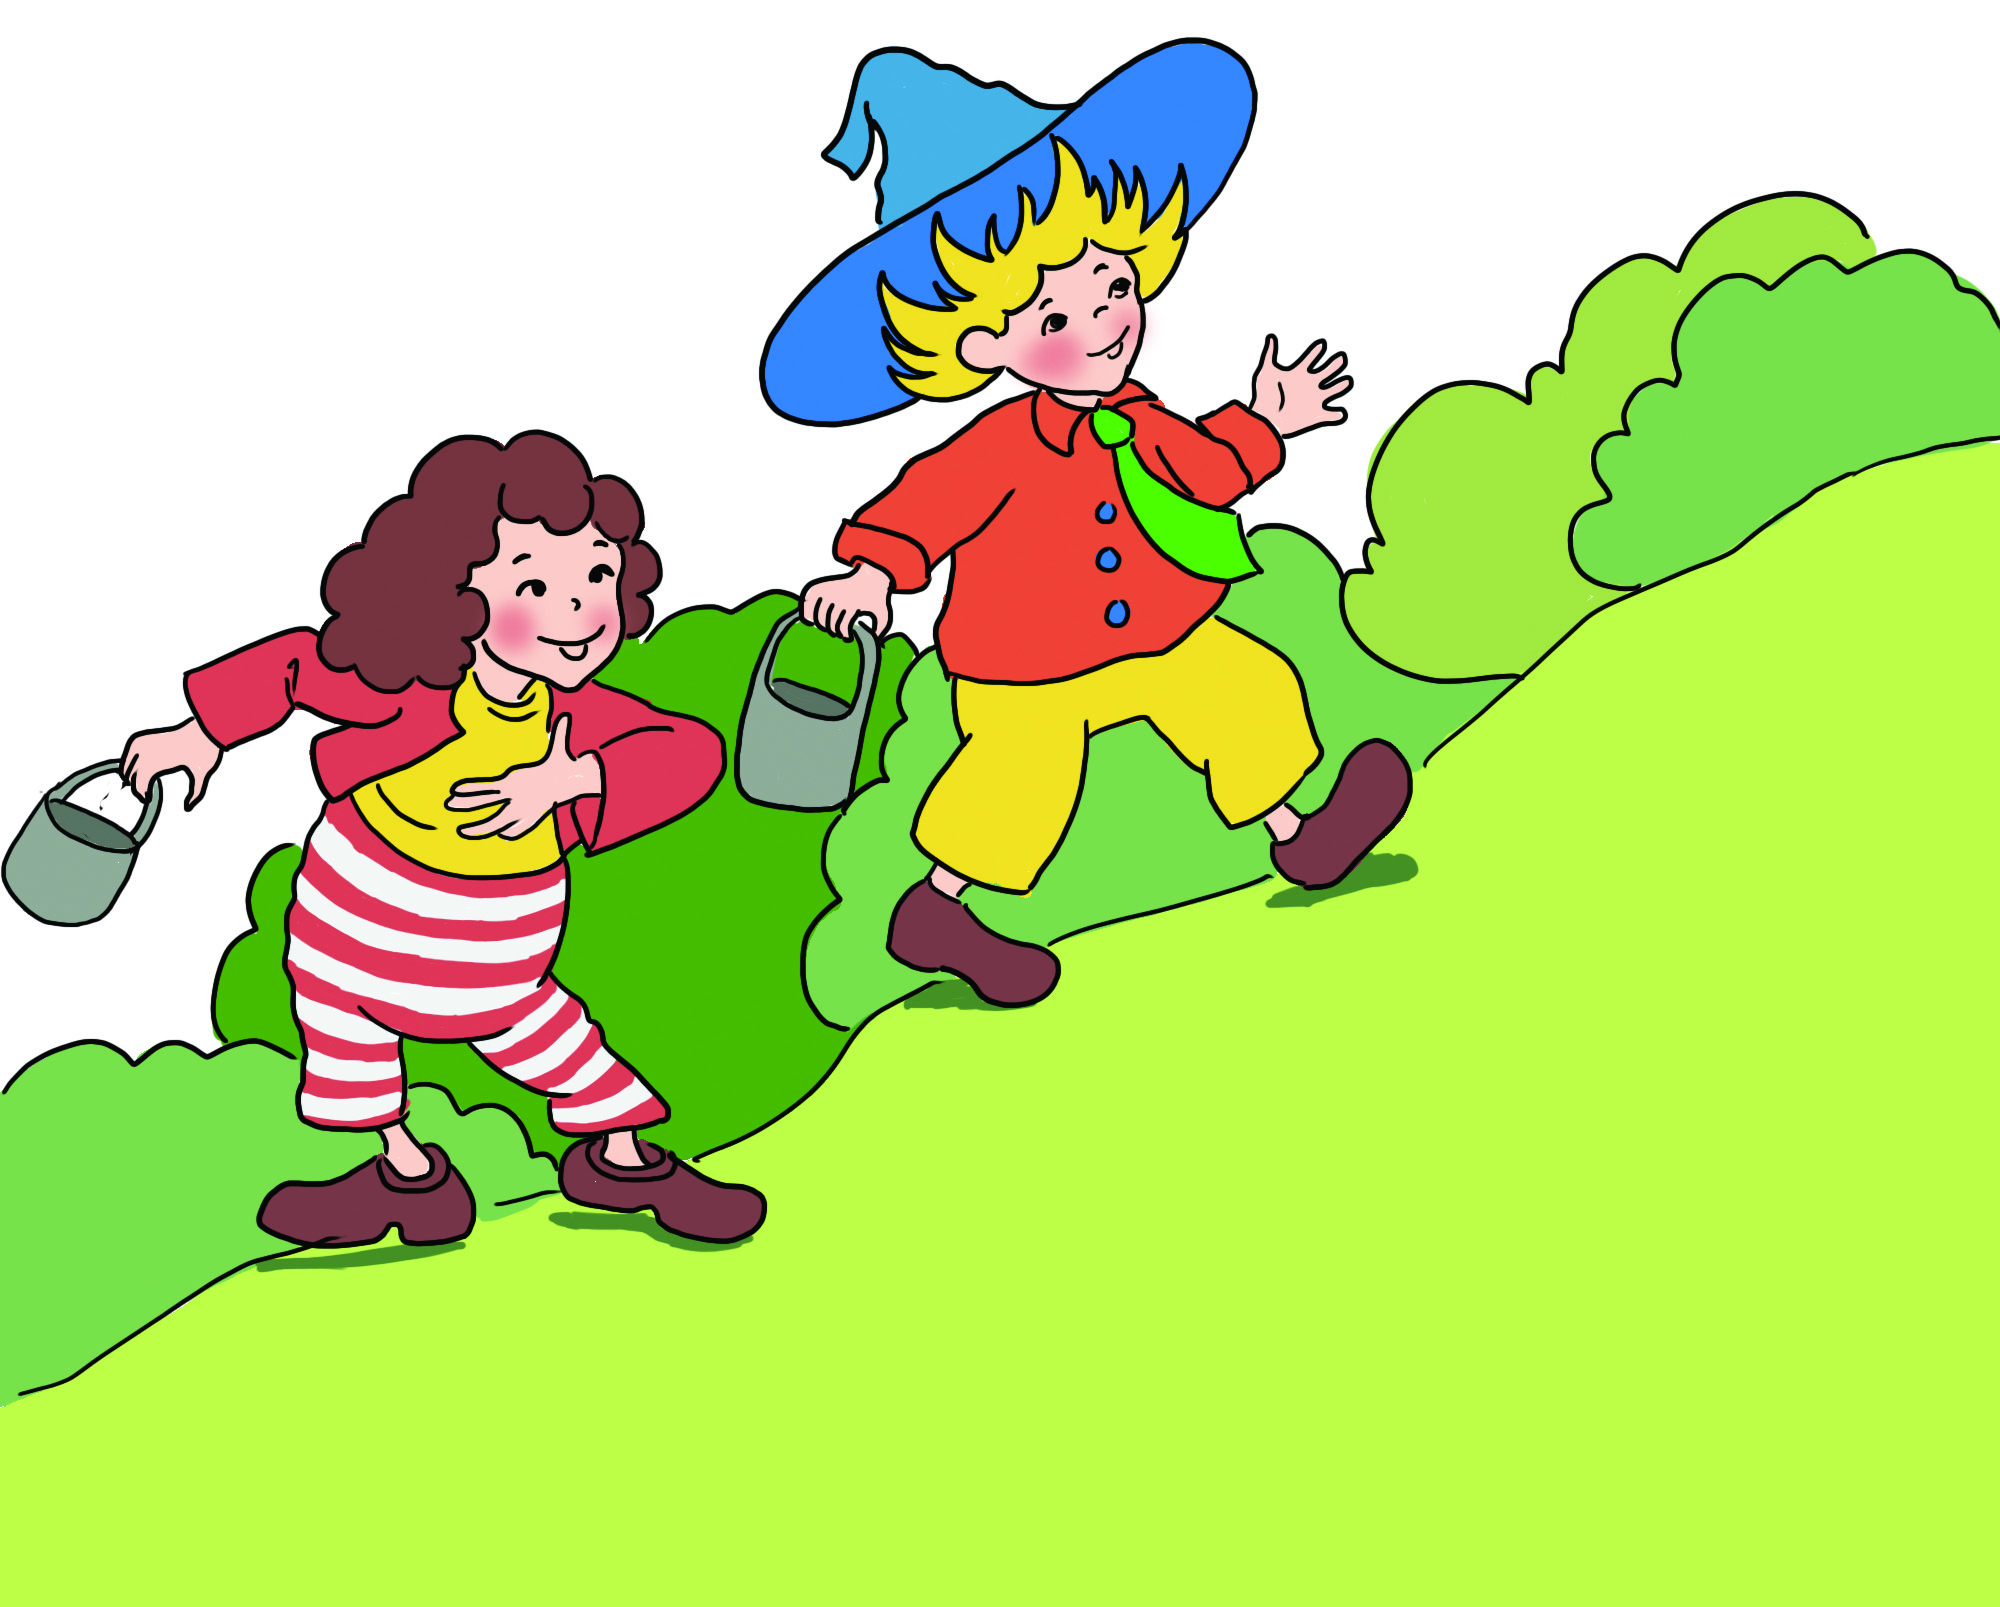
\includegraphics[width=1\linewidth]{Hinh8_LayNhua}
		%\caption{\textit{\color{toancuabi}Hình $8$.}}
		\vspace*{-15pt}
	\end{wrapfigure}
	\textbf{\color{toancuabi}Câu chuyện $\pmb{6.}$} Sau khi làm xong quả kinh khí cầu, Biết Tuốt còn bảo các chú tí hon chuẩn bị cát mang lên kinh khí cầu, làm dù để phòng sự cố xảy ra khi đang bay. Không những thế Biết Tuốt còn hướng dẫn các bạn luyện tập những thao tác cần thiết trước khi lên đường. Buổi sáng hôm đó, các chú tí hon dạy từ sáng sớm và bắt đầu luyện tập từ $7$ giờ. Các chú mất $25$ phút học cách đứng thăng bằng trên kinh khí cầu, mất $\frac{3}{4}$ giờ để xếp các bao cát và ném bao cát xuống khi cần thiết và $1\frac{1}{2}$ để học cách nhảy dù. Các chú đã luyện tập không ngừng nghỉ suốt từ $7$ giờ $40$ phút sáng, mấy giờ các chú ấy mới luyện tập xong các bạn nhỉ?
	\begin{multicols}{2}
		\begin{figure}[H]
			\centering
			\vspace*{-5pt}
			\captionsetup{labelformat= empty, justification=centering}
			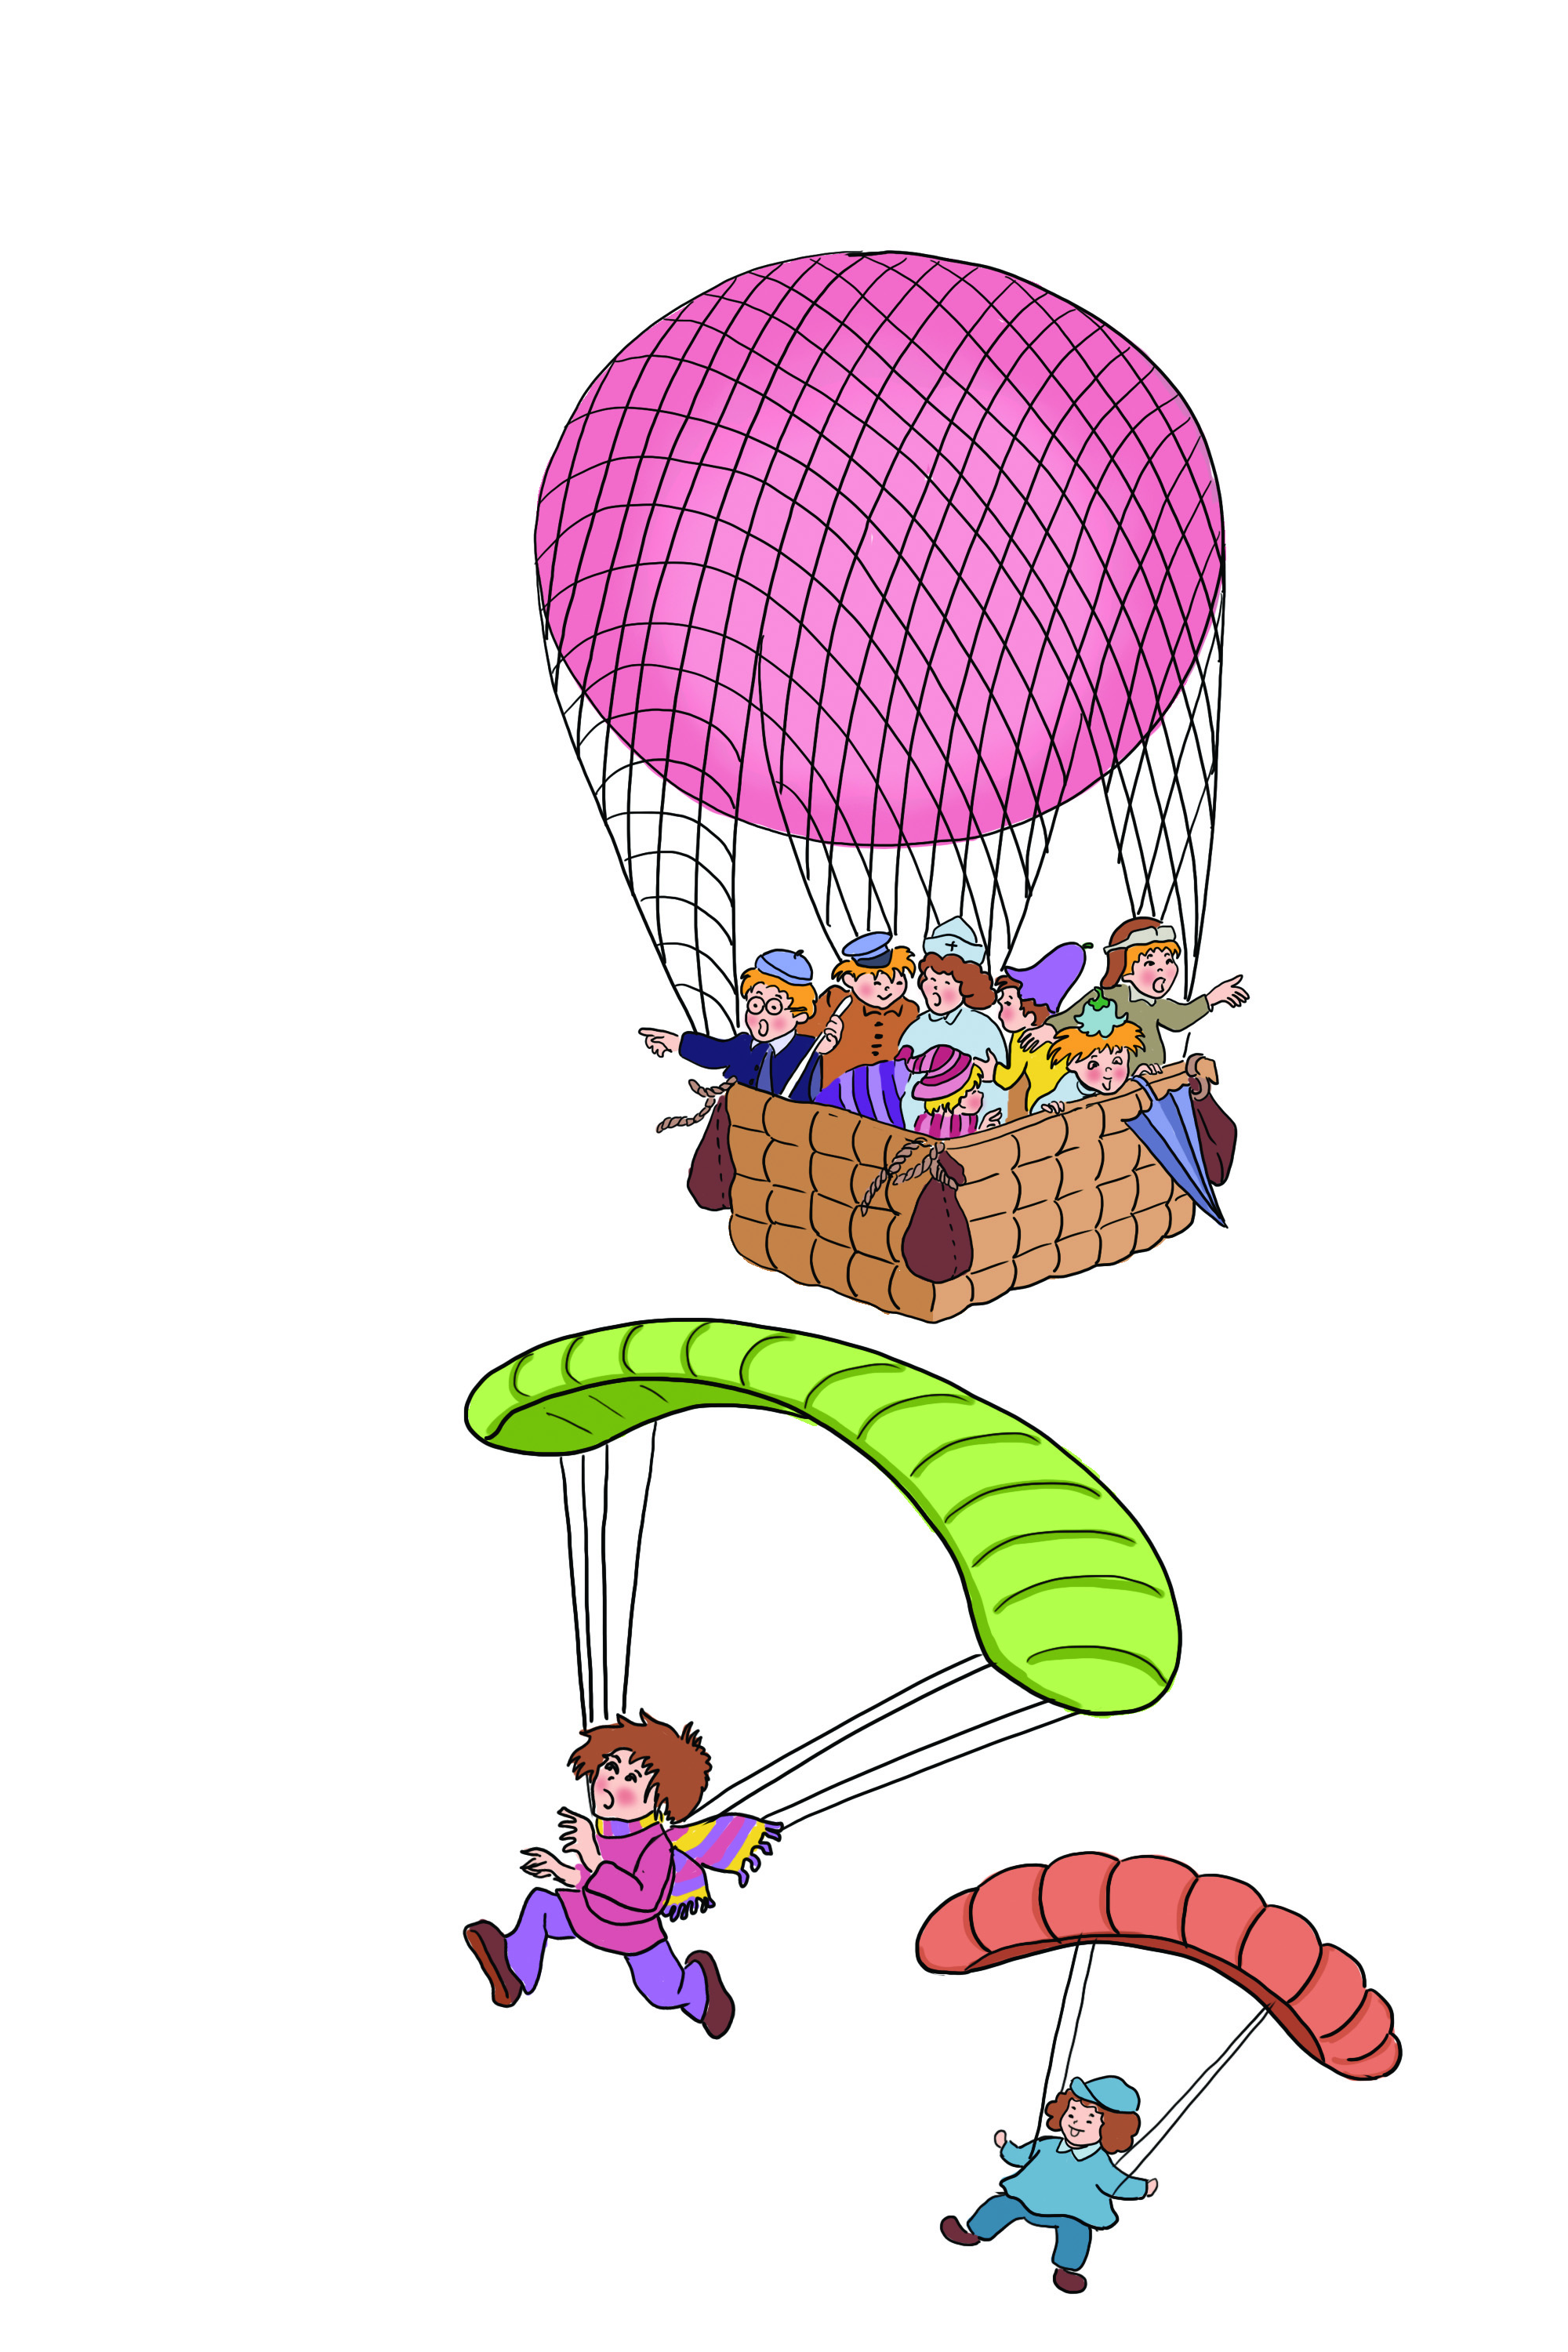
\includegraphics[width=0.98\linewidth]{Hinh9_KinhKhiCau}
			%\caption{\textit{\color{toancuabi}Hình $9$.}}
			\vspace*{-5pt}
		\end{figure}
		\textbf{\color{toancuabi}Câu chuyện $\pmb{7.}$} Ngày khởi hành cũng đã đến, các chú tí hon khăn gói quả mướp, háo hức lên đường. Quả cầu vút lên cao một cách êm ả, nó lên cao, rất cao, các chú tí hon sung sướng ngắm nhìn cảnh phía dưới. Quả cầu vượt qua bao ruộng đồng, bay qua dòng sông Dưa Chuột, vượt qua những rặng núi, xuyên qua những đám mây. Chắc Chắn được giao ghi lại lịch trình của chuyến đi, một tay chú cầm bút ghi, tay kia cầm chiếc đồng hồ, \,\,chú \,\,nói: Chúng\,\, ta\,\, khởi
	\end{multicols}
	hành lúc $8$ giờ và mất $40$ phút từ lúc đi đến lúc bay qua dòng sông Dưa Chuột, chúng ta mất thêm $60$ phút để bay qua nhiều ruộng đồng rồi đến một dãy núi, ở đây ta phải dừng lại mất $10$ phút để bỏ bớt một số bao cát giúp kinh khí cầu bay cao hơn.  Mình đã mất $80$ phút để bay qua dãy núi này. Khi vừa bay qua dãy nũi, chúng ta gặp những đám mây trắng bồng bềnh trôi, và kinh khí cầu vừa bay qua được những đám mây này mất $20$ phút. Theo kế hoạch $1$ giờ $30$ phút chiều mình sẽ tới một hòn đảo.
	\vskip 0.1cm
	\begin{wrapfigure}{r}{0.5\linewidth}
		\centering
		\vspace*{-25pt}
		\captionsetup{labelformat= empty, justification=centering}
		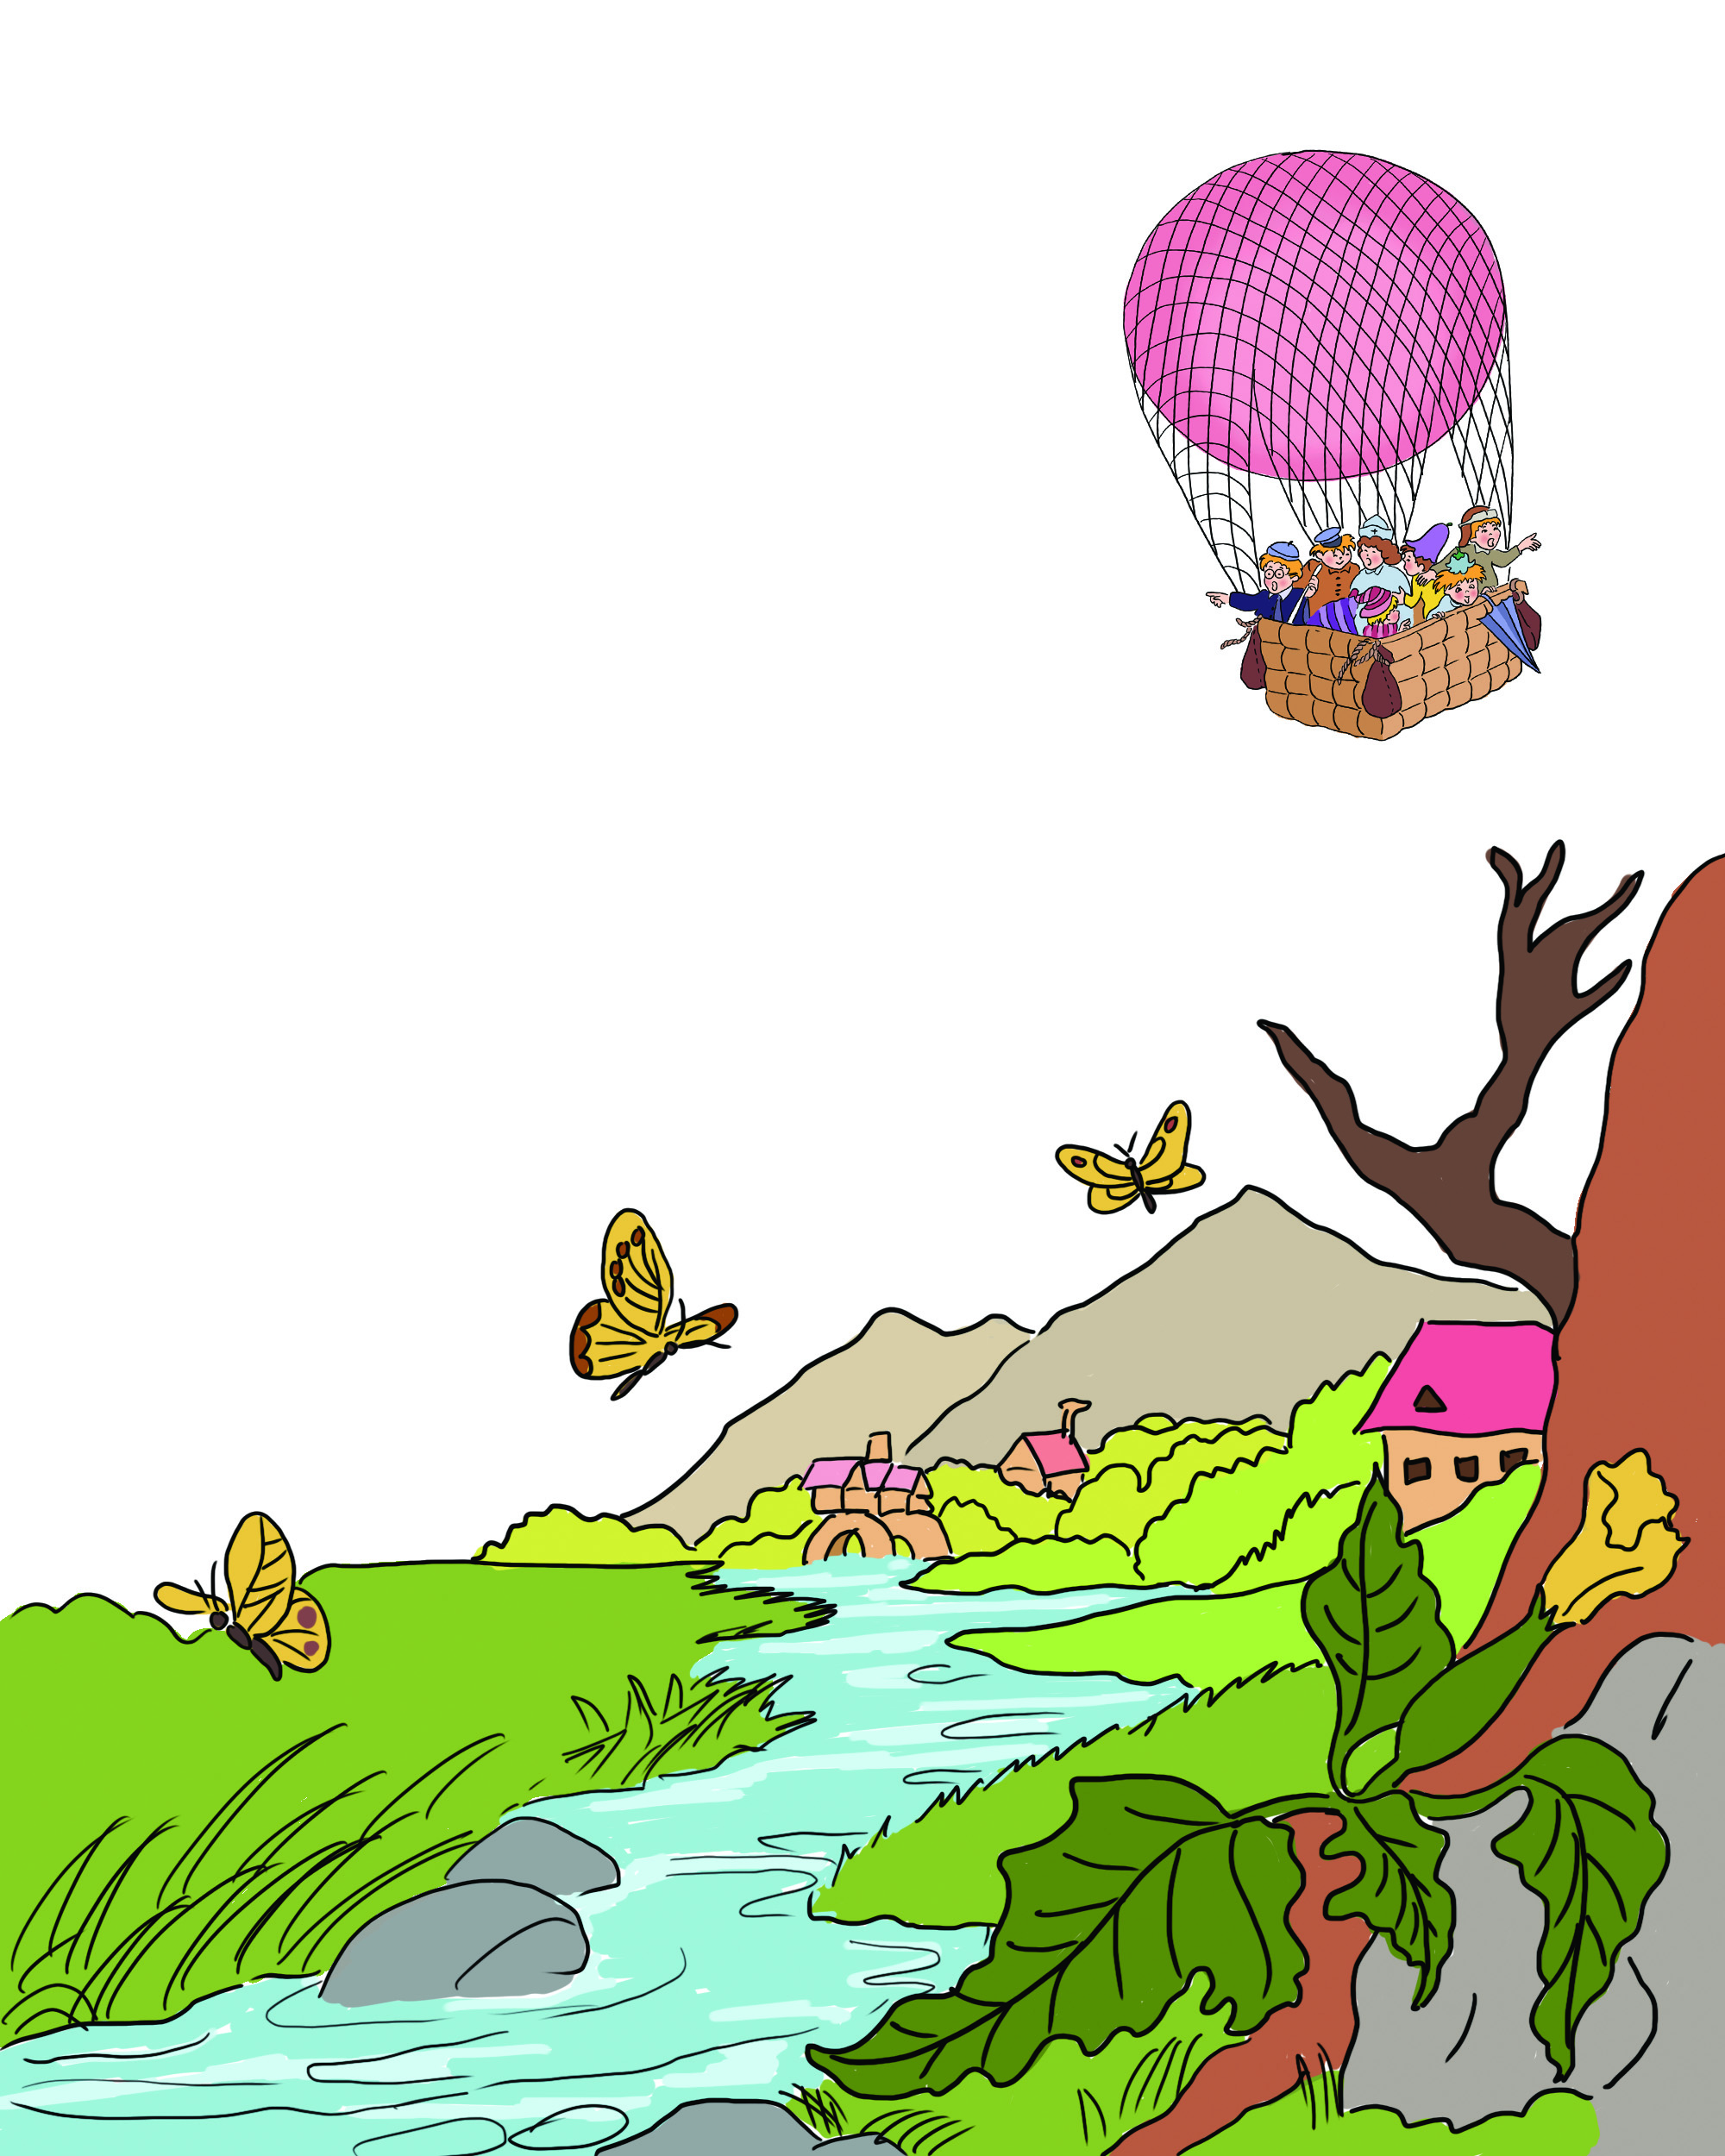
\includegraphics[width=1\linewidth]{Hinh23_KinhKhiCau}
		%\caption{\textit{\color{toancuabi}Hình $9$.}}
		\vspace*{-20pt}
	\end{wrapfigure}
	Cáu Kỉnh lên tiếng: Cậu kể dài dòng quá, tôi cần quan tâm còn bao lâu nữa thì chúng ra sẽ đến được hòn đảo. Chắc Chắn mới tập trung ghi chép thôi, chưa có tính ra yều cầu của Cáu Kỉnh, các bạn giúp Chắc Chắn nhé. 
	\vskip 0.1cm
	\textbf{\color{toancuabi}Câu chuyện $\pmb{8.}$} Kinh khí cầu đã đưa các chú tí hon dạo chơi trên chín tầng mây được hơn một ngày. Bao giờ thì đến thành phố mới lạ theo kế hoạch nhỉ? Biết Tuốt nói với các bạn:
	\vskip 0.1cm
	“\textit{Kinh khí cầu sẽ không đưa ta ngay lập tức đến thành phố mới mà sau một …}”, Biết Tuốt ngập ngừng. Các chú tí hon liền nhao nhao đoán: “\textit{một giây!}”, “\textit{một phút!}”, “\textit{một giờ!}”,“\textit{một ngày!}”, “\textit{một tuần!}”, “\textit{một tháng!}” Biết Tuốt nói rằng trong các câu trả lời trên thì một dự đoán là chính xác so với tính toán của cậu ấy, còn các dự đoán còn lại lần lượt sai $24$ lần, $60$ lần, $168$ lần, $720$ lần, và $3600$ lần so với tính toán. Theo tính toán của Biết Tuốt thì bao lâu nữa các bạn của chúng ta sẽ đến được thành phố mới nhỉ?
	\vskip 0.1cm
	Không biết bao lâu thì các chú tí hon mới đến thành phố mới lạ, nhưng các cô chú hon ở nhà thì ngưỡng mộ Biết Tuốt và các bạn ấy lắm. Cả thành phố ngâm nga suốt bài thơ của thi sĩ Hoa Giấy
	
	\begin{adjustwidth}{75pt}{0pt}
		\begin{flushleft}
			\textit{Quả cầu vĩ đại căng hơi\\
			Trời cao vút tới, bồi hồi lòng ta\\
			Tự hào như cánh chim xa\\
			Tầng không ta vượt, bay qua ruộng đồng\\
			Bay qua biển, bay qua sông\\
			Chúng ta đâu có nản lòng bạn ơi!}
		\end{flushleft}
	\end{adjustwidth}
	\begin{center}
		\textbf{\color{toancuabi}Những người bạn mới}
	\end{center}
	\textit{Chuyến đi trên kinh khí cầu đã không đúng như dự định vì giữa đường các bạn gặp tai nạn và cả đoàn đã phải nhảy dù ra khỏi kinh khí cầu. Các chú tí hon đã lạc đến thành phố Xanh và được các cô tí hon ở đây giúp đỡ. Thành phố Xanh có những ngôi nhà xinh đẹp, không gian ngợp trong màu lá cây xanh thắm, phố xá luôn sạch sẽ, gọn gàng. Từ tai nạn không may này mà các chú đã được làm quen với những cô tí hon hết sức dễ thương như Mắt Xanh, Bạch Tuyết, biết đến thi sĩ Hoa Dại, hay bác sĩ Mật Ngọt, …  Không những thế các chú còn được làm quen với các chú tí hon ở thành phố Diều, biết đến Đinh Ốc, nhà phát minh cừ khôi với rất nhiều phát minh kì lạ và cả nhà văn Cả Láu với những câu chuyện thú vị từ chiếc máy ghi âm.}
	\begin{figure}[H]
		\centering
		\vspace*{-5pt}
		\captionsetup{labelformat= empty, justification=centering}
		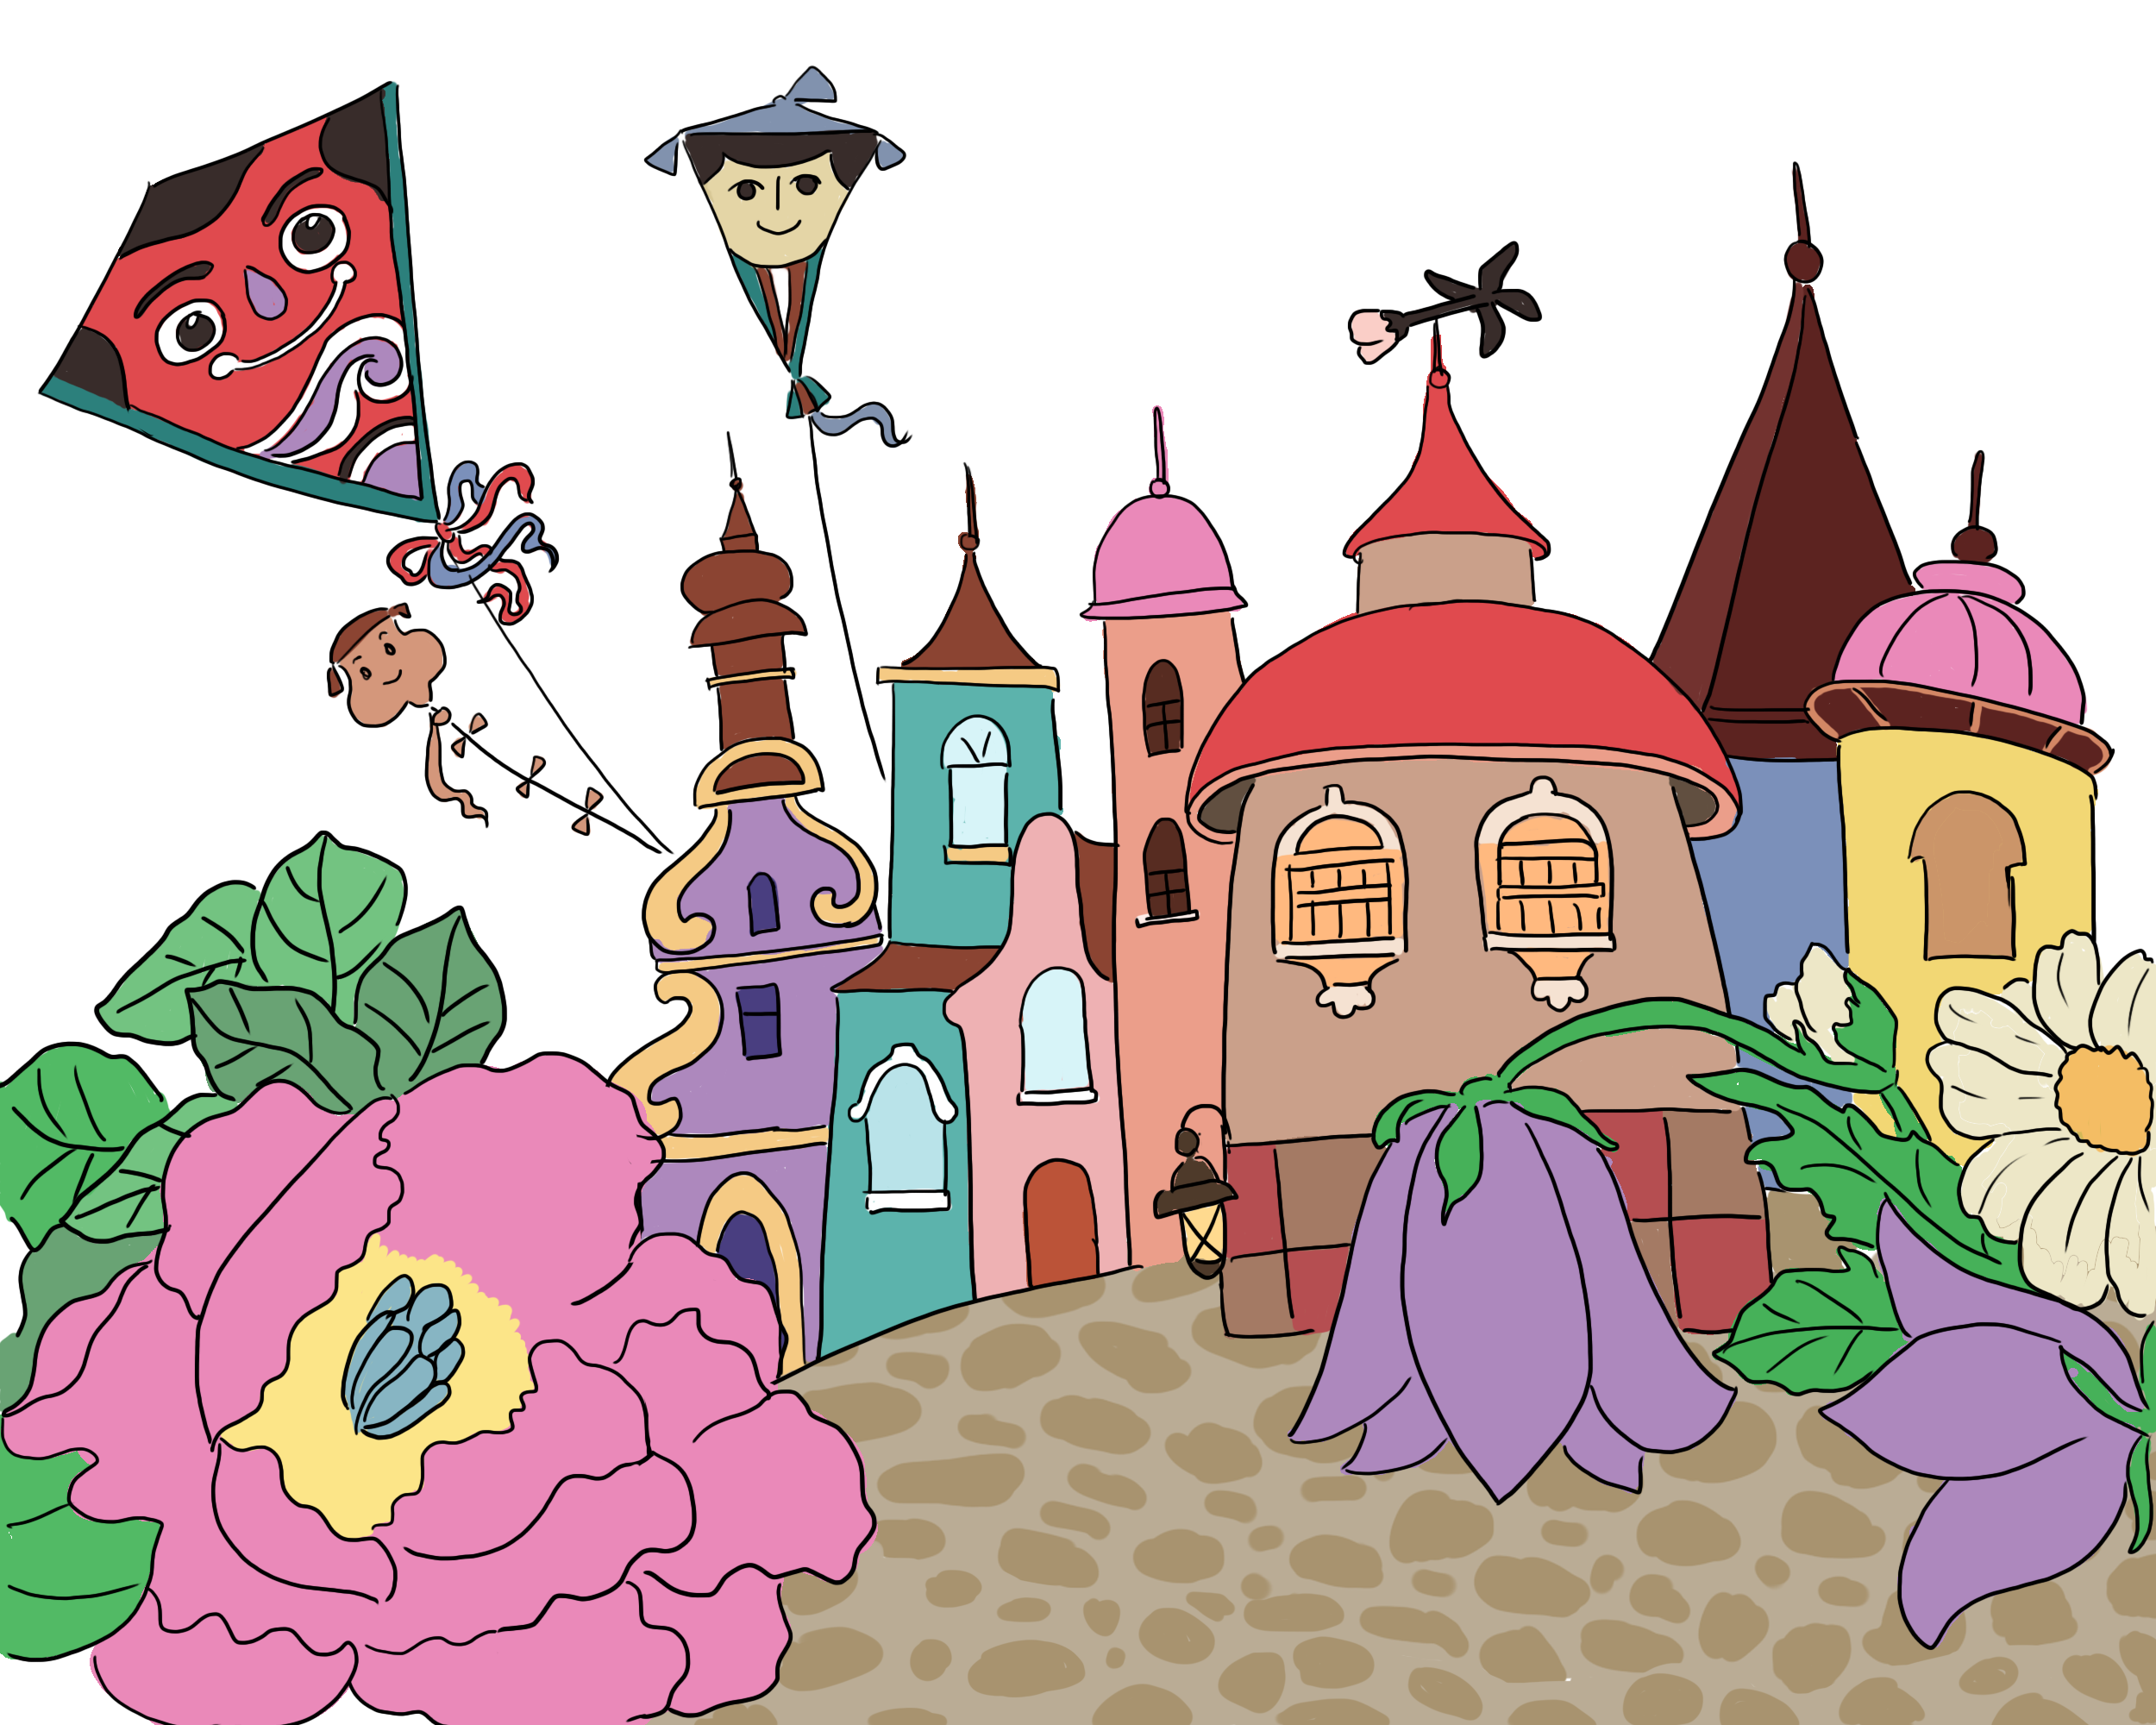
\includegraphics[width=0.5\linewidth]{Hinh11_ThanhPhoDieu}
		%\caption{\textit{\color{toancuabi}Hình $9$.}}
		\vspace*{-10pt}
	\end{figure}	
	Chúng ra cùng tham gia vào những câu chuyện của các cô chú tí hon ở hai thành phố xinh đẹp này qua những bài toán sau nhé.
	\vskip 0.1cm
	\textbf{\color{toancuabi}Câu chuyện $\pmb{9.}$} Các cô tí hon có một chiếc xe ô tô nhưng bị hỏng. Bu Loong và Đinh Vít đã quyết định sửa giúp các cô chiếc ô tô này. Do  không có đồ nghề để sửa, thế nên hai cậu sang thành phố Diều để mượn. Chú tài xế Bánh Vòng đã chở hai cậu đến nhà Đinh Ốc để mượn mỏ hàn. Nhà của Đinh Ốc nằm trên một căn phố nhỏ. Có $5$ ngôi nhà liên tiếp được đánh số lần lượt từ $1$ đến $5$ ở phố của Đinh Ốc và nhà của cậu ấy là nhà số $3$. Khi đến nơi, những chú tí hon thấy cả năm ngôi nhà có các màu sơn khác nhau: xanh, đỏ, tím, vàng, hồng. Ngôi nhà màu đỏ chỉ nằm cạnh một ngôi nhà khác. Ngôi nhà màu xanh thì nằm cạnh các ngôi nhà màu vàng và màu đỏ. Nhà của Đinh Ốc màu gì các bạn có biết không?
		\begin{figure}[H]
		\centering
		\vspace*{-5pt}
		\captionsetup{labelformat= empty, justification=centering}
		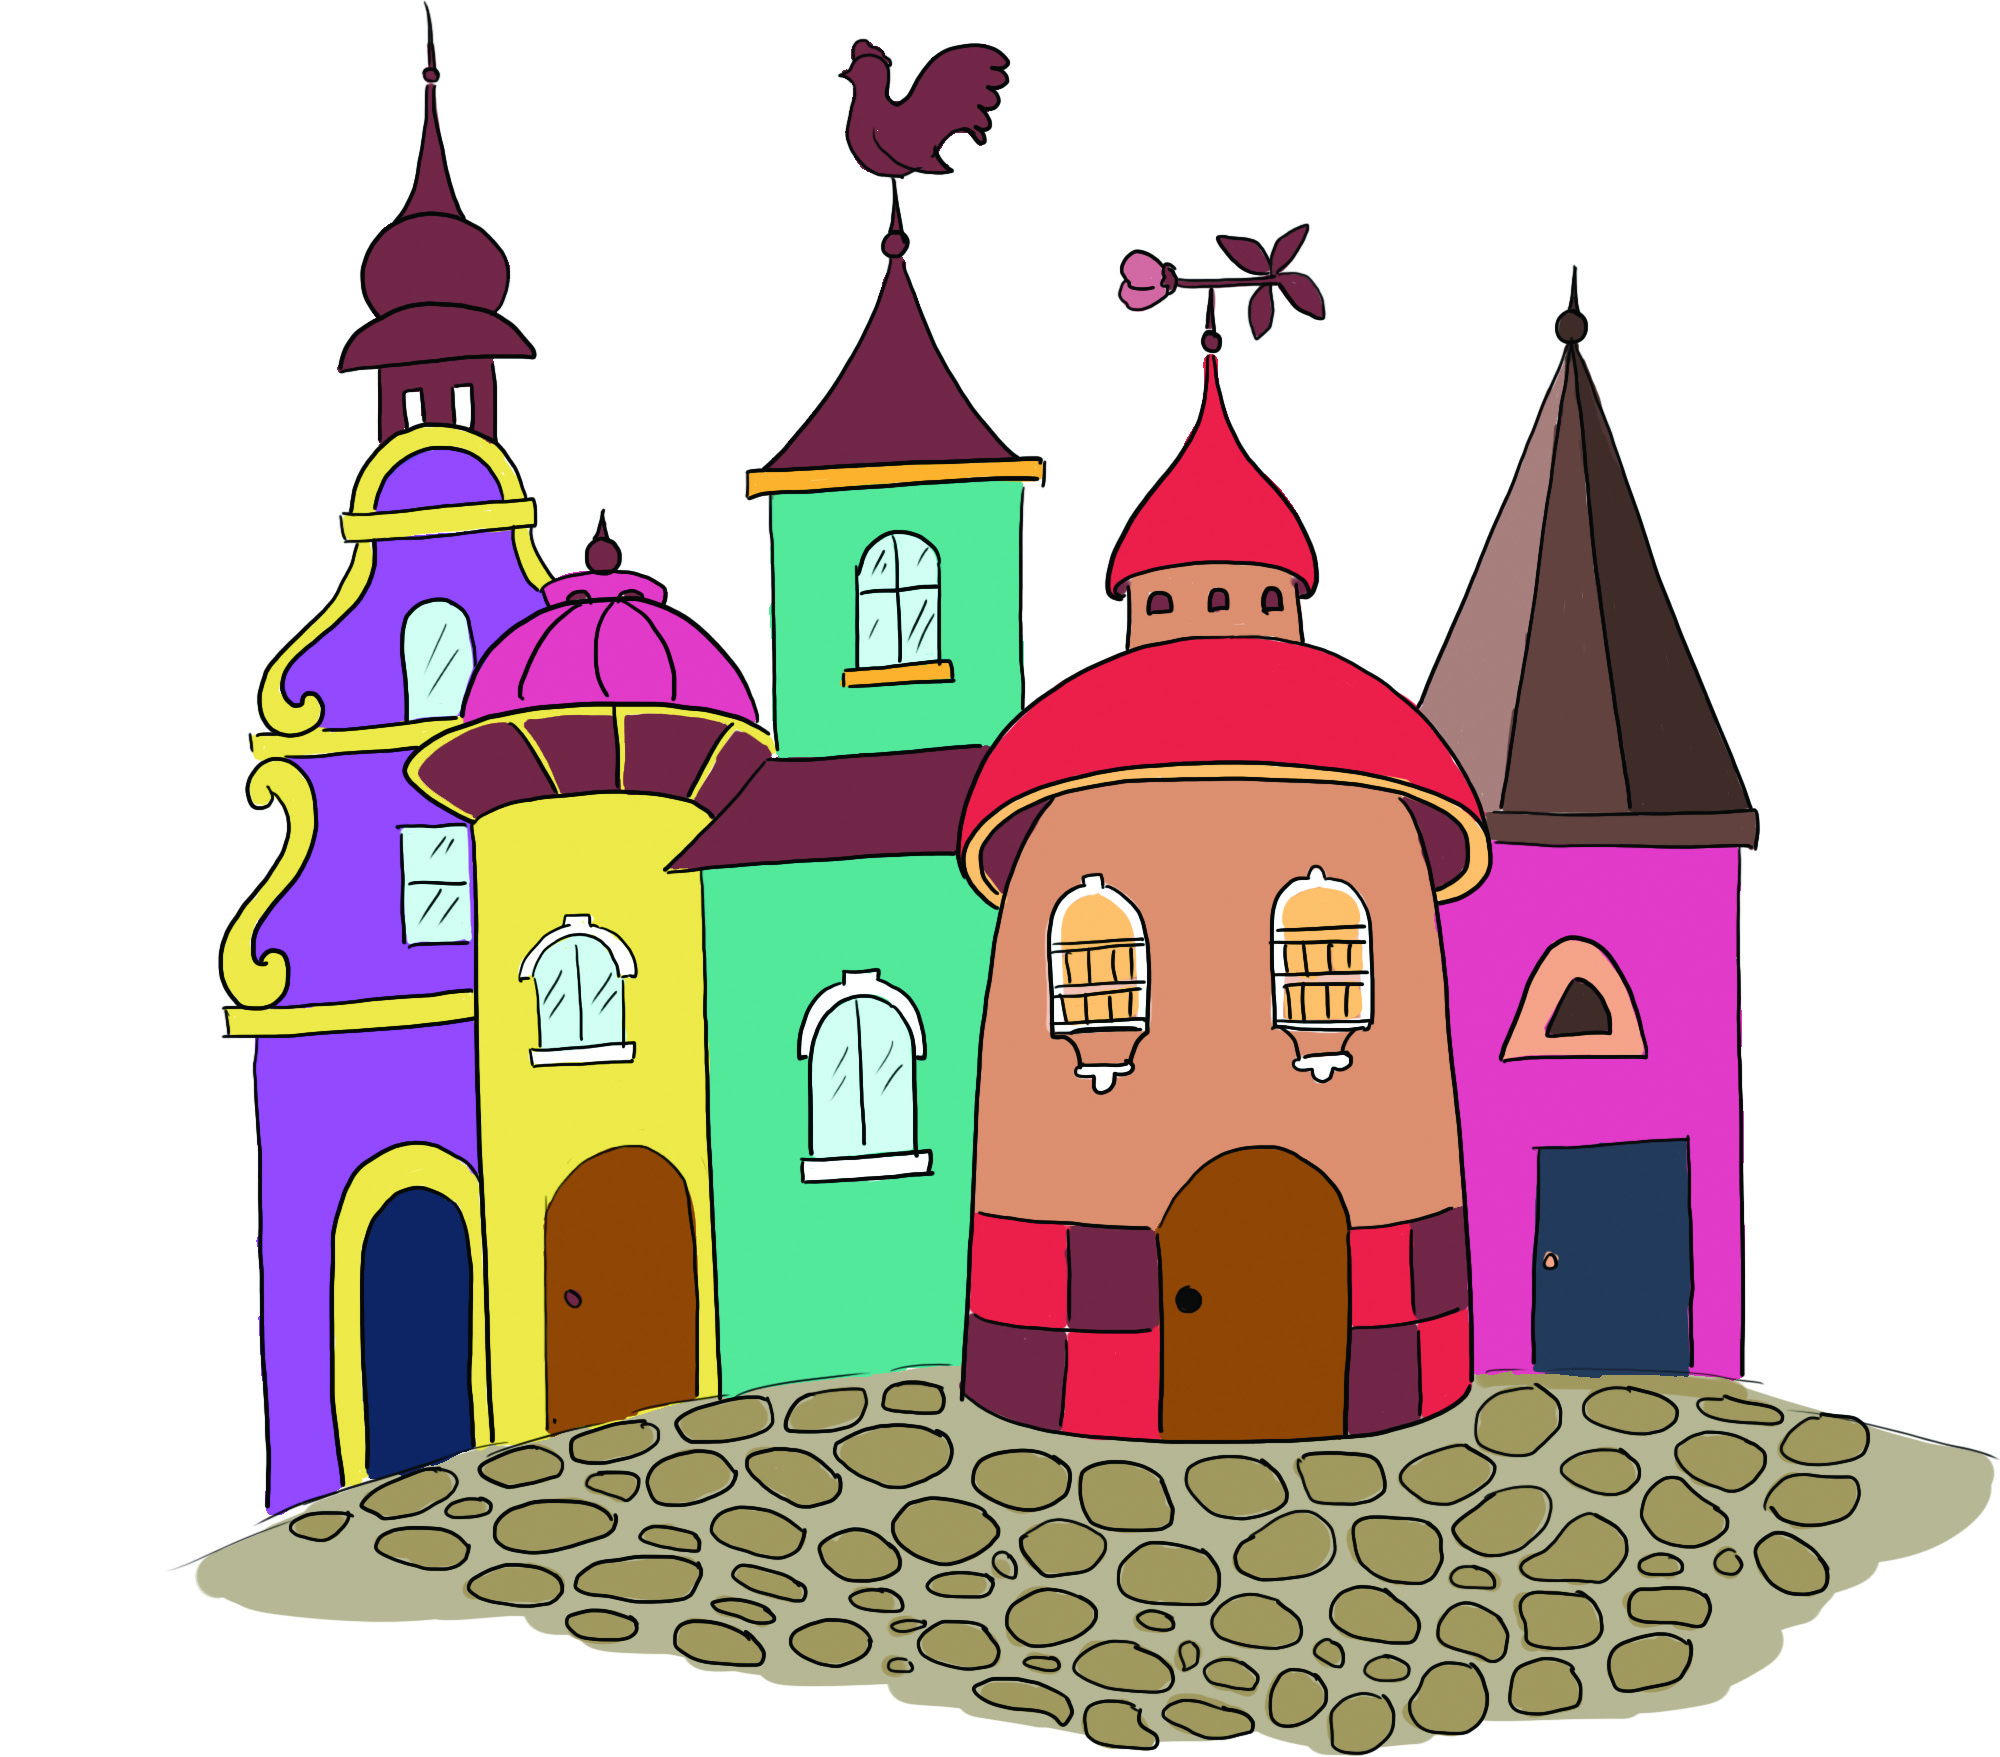
\includegraphics[width=0.6\linewidth]{Hinh24_NhaDinhOc}
		%\caption{\textit{\color{toancuabi}Hình $11$.}}
		\vspace*{-10pt}
	\end{figure}
	\textbf{\color{toancuabi}Câu chuyện $\pmb{10.}$} Ở thành phố Xanh, mỗi nhà có một hầm để chứa hoa quả. Các cô tí hon cưa các loại quả từ cây xuống và lăn về hầm, công việc khá là tốn thời gian và công sức. Nhờ có Bu Loong và Đinh Vít đã sửa chiếc ô tô mà việc vận chuyển được “cơ giới hóa”, giúp hoa quả được đưa về hầm nhanh hơn. Một ngày nọ nhóm bốn chú tí hon vận chuyển được $100$ quả táo về hầm. Mít Đặc nói: “ Tớ vận chuyển được trên $5$ quả táo đấy, nhưng tớ vẫn chuyển ít hơn Ngộ Nhỡ”. Nhanh Nhảu thì hí hửng khoe: “Thế mà tớ chuyển được hơn Ngộ Nhỡ $3$ quả đấy”. Bu Loong nói ngay: “Các cậu chuyển được nhiều táo đấy, nhưng nhờ cơ giới hóa mà số táo tớ mang về hầm gấp $3$ lần tổng số táo của cả ba cậu.” Các bạn tính xem mỗi chú tí hon vận chuyển được bao nhiêu táo nhé.
	\begin{figure}[H]
		\centering
		\vspace*{-5pt}
		\captionsetup{labelformat= empty, justification=centering}
		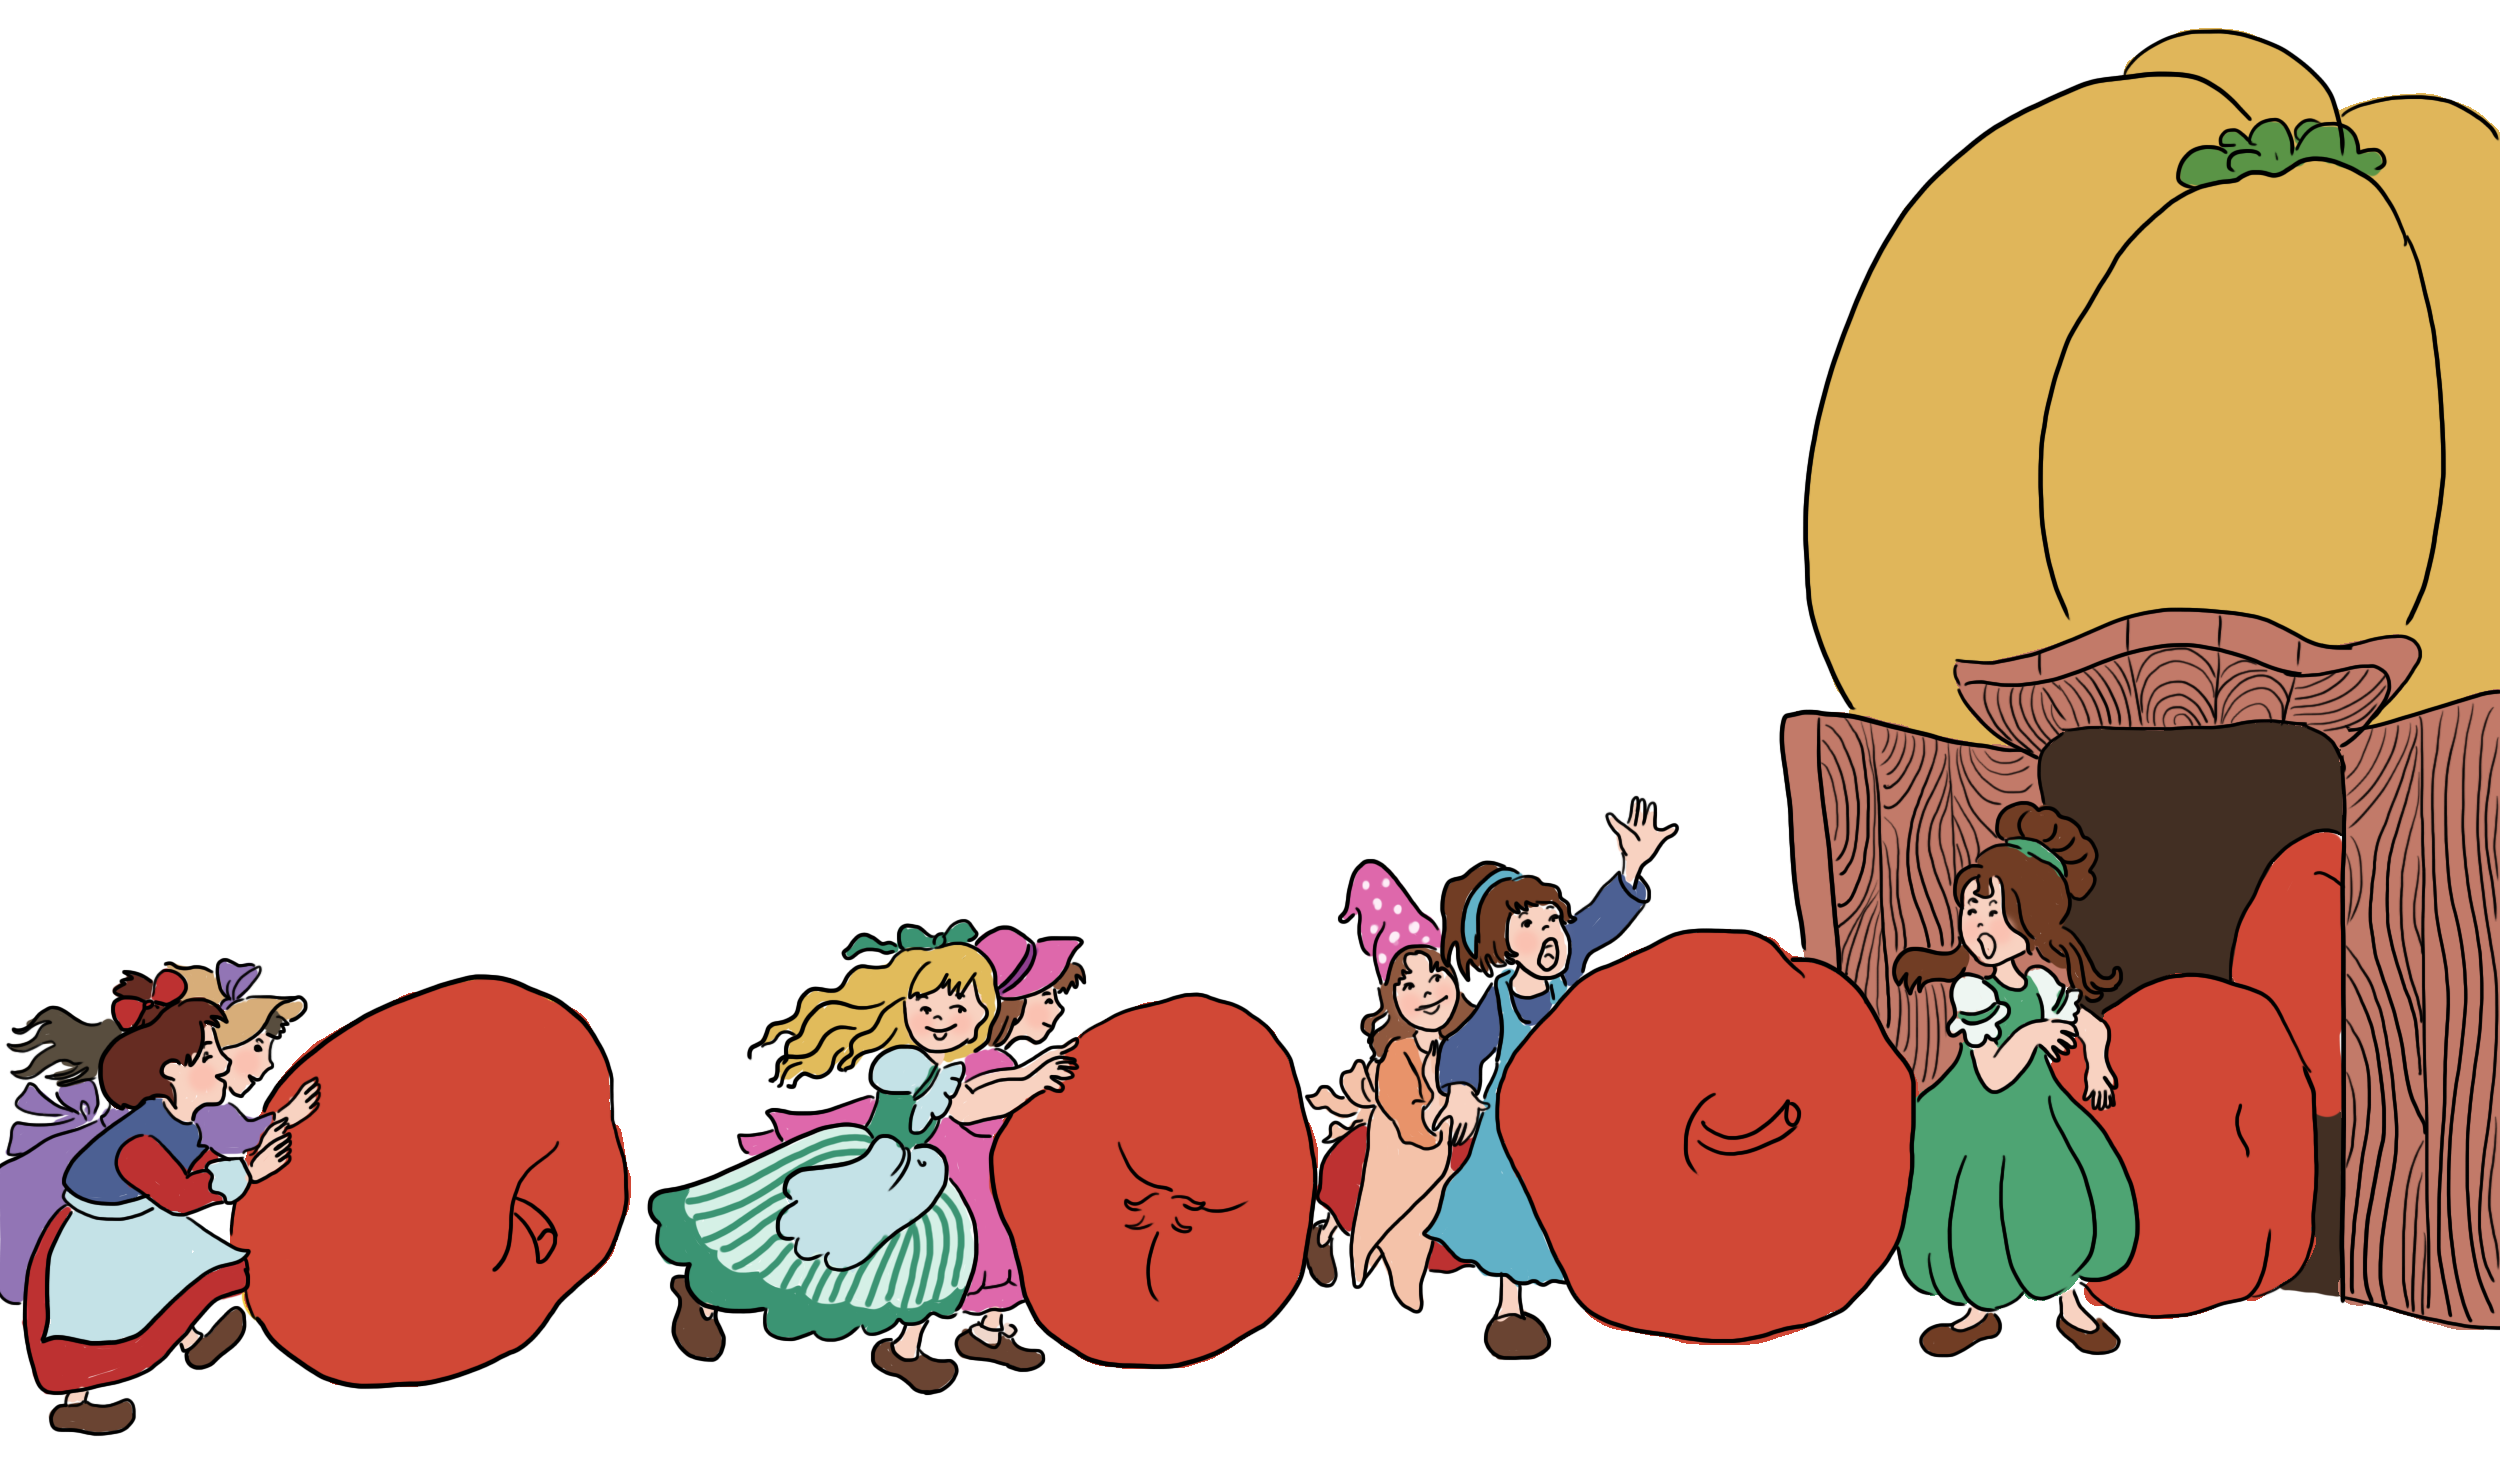
\includegraphics[width=0.6\linewidth]{Hinh12_ChuyenTao}
		%\caption{\textit{\color{toancuabi}Hình $12$.}}
		\vspace*{-10pt}
	\end{figure}
	\textbf{\color{toancuabi}Câu chuyện $\pmb{11.}$} Nhờ có cơ giới hóa mà công việc tiến hành dễ dàng và mau chóng. Ô tô đi lại như con thoi giữa các cây táo. Các cô tí hon không phải đẩy quả về nhà nữa nhưng không phải vì thế mà các cô ngồi chơi. Các cô đã dựng hai cái lều vải ở trong phố và đem đến nước đường và bánh mứt kẹo cho bà con lao động có thể giải khát lúc nghỉ ngơi.Lều lớn chứa được lượng người nhiều gấp đôi so với phòng nhỏ. Vào một buổi trưa,ba phần tư chỗ ngồi của hai cái lều đã kín chỗ. Sau đó, một nhóm gồm $18$ cô chú tí hon lại ghé đến lều. Thế nhưng, một cô tí hon ra thông báo rằng lều chỉ còn đủ chỗ cho một nửa số người của nhóm. Các bạn có tính được mỗi lều chứa được bao nhiêu người không?
		\begin{figure}[H]
		\centering
		\vspace*{-5pt}
		\captionsetup{labelformat= empty, justification=centering}
		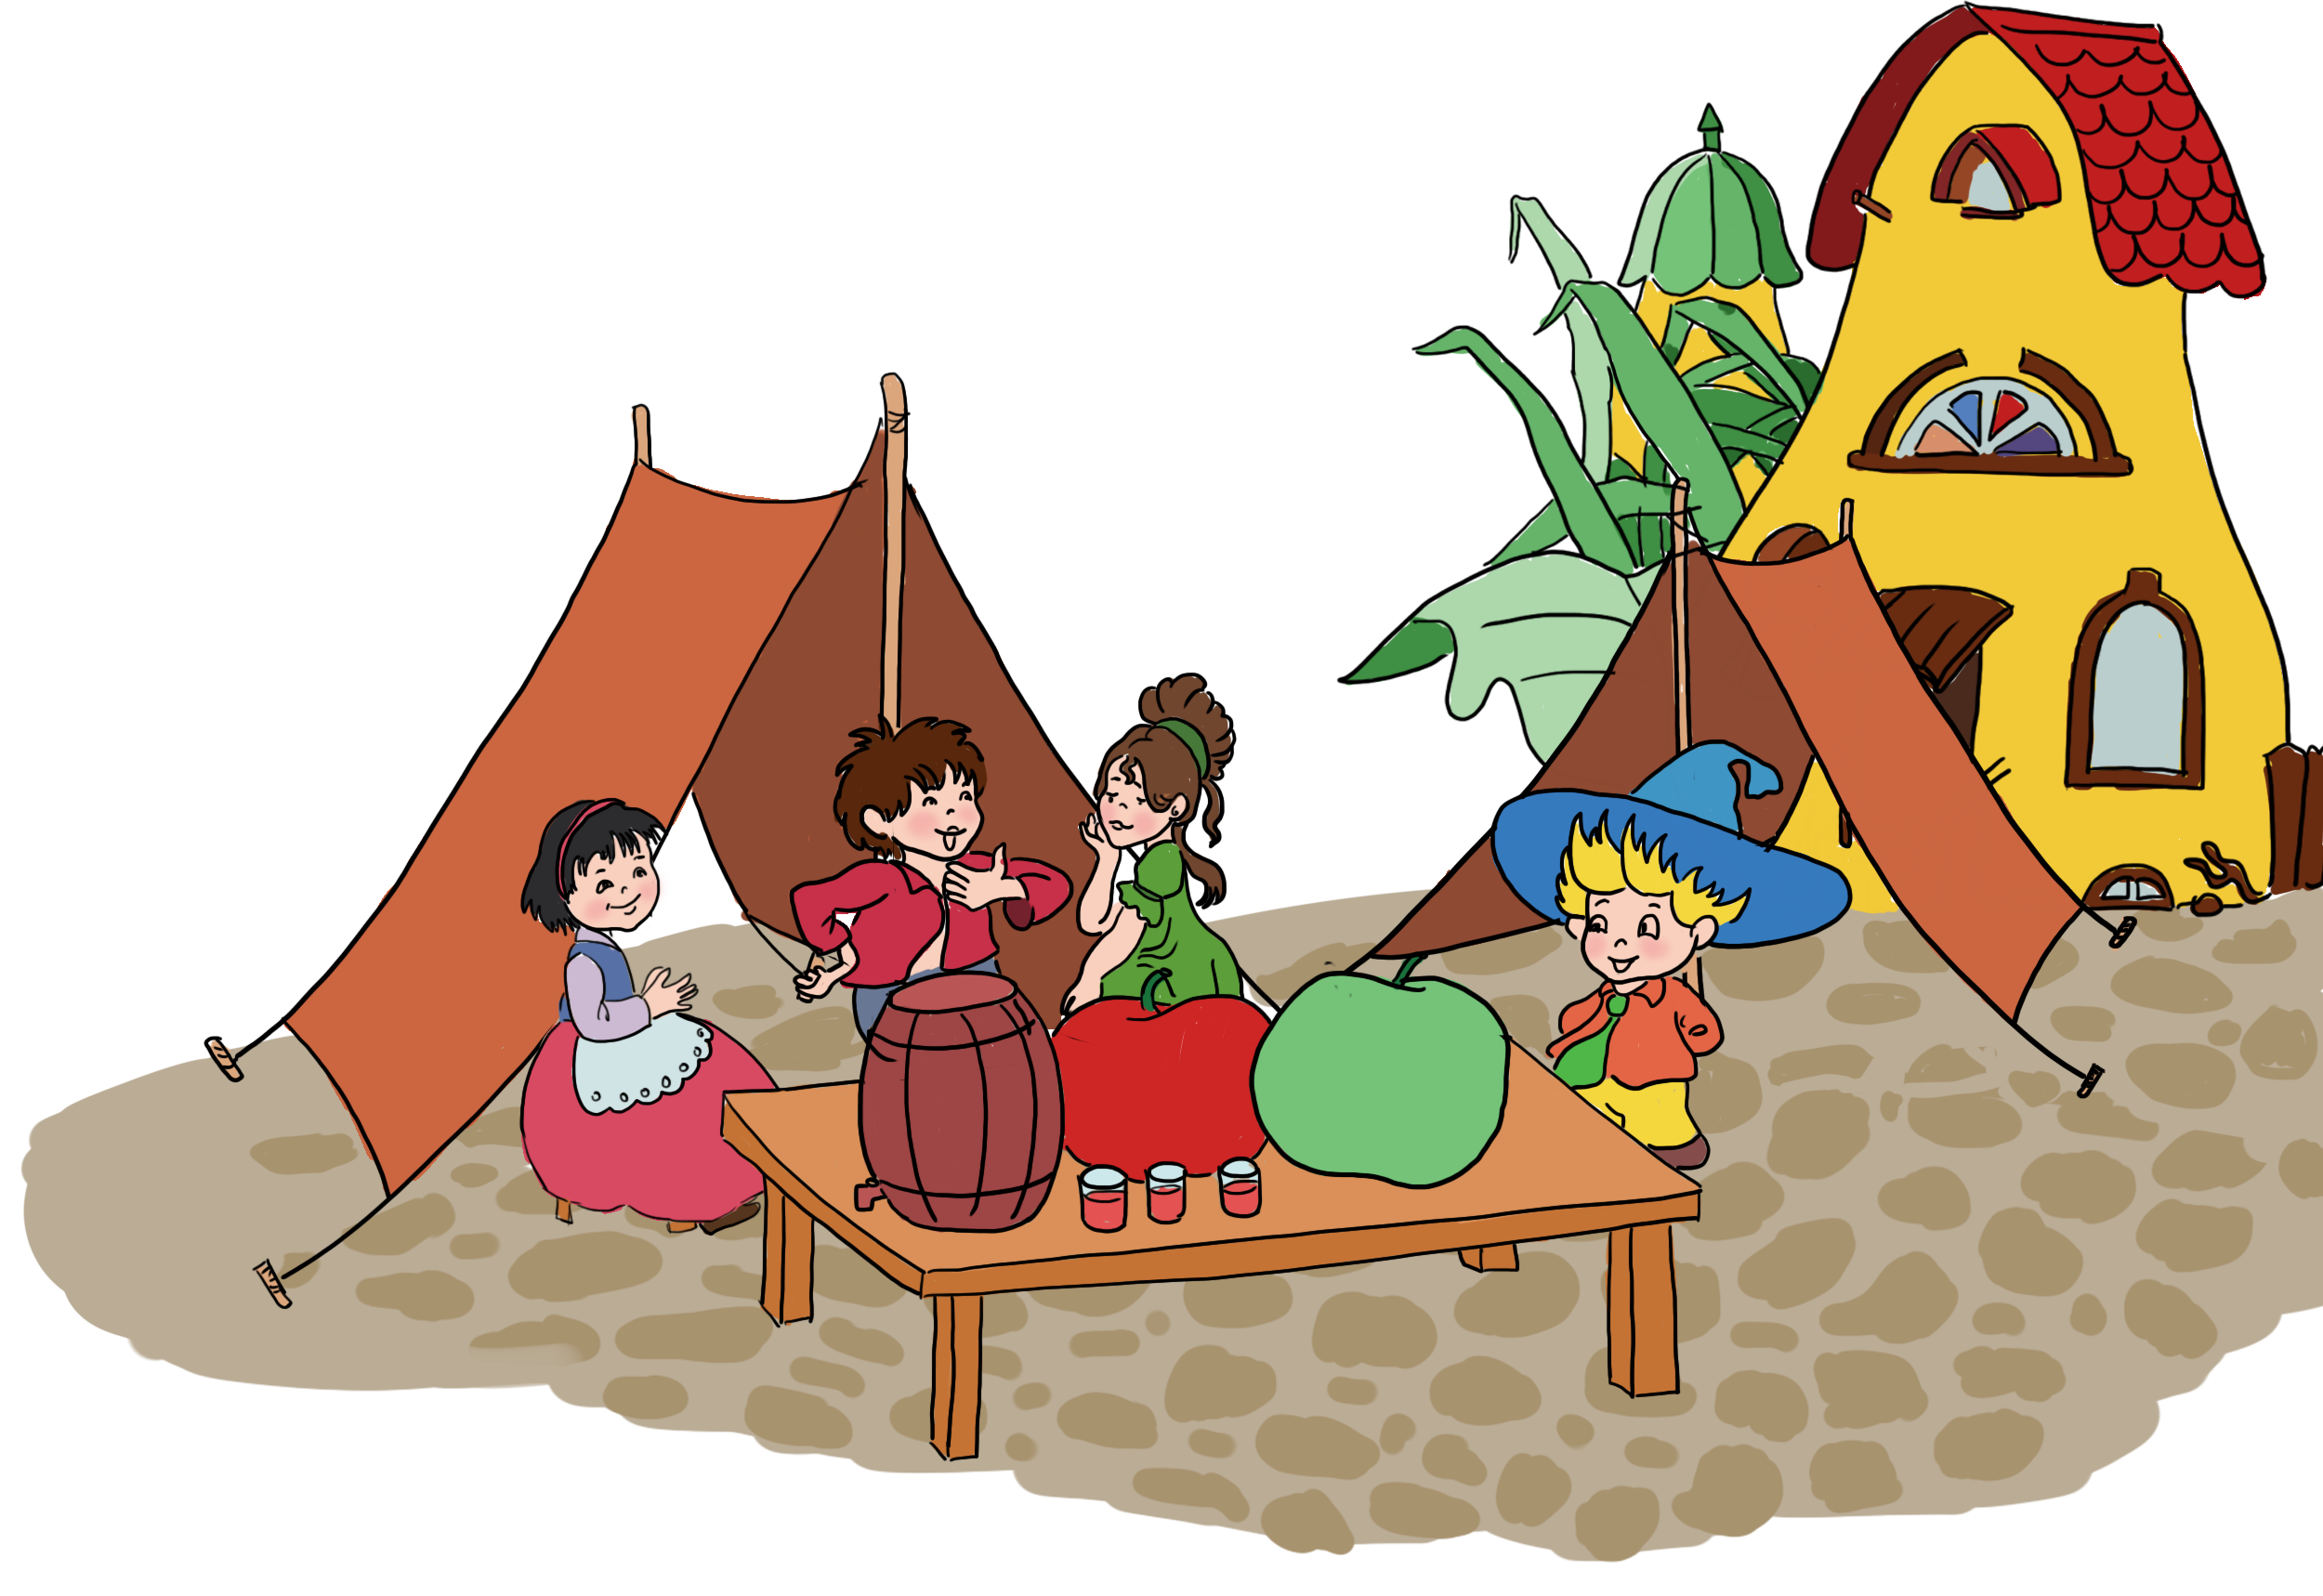
\includegraphics[width=0.55\linewidth]{Hinh13_Leu}
		%\caption{\textit{\color{toancuabi}Hình $13$.}}
		\vspace*{-10pt}
	\end{figure}
	\textbf{\color{toancuabi}Câu chuyện $\pmb{12.}$} Bánh Vòng khi đưa Bu Loong và Đinh Vít trở về thành phố Xanh đã ở lại hỗ trợ các cô tí hon chuyển hoa quả, rồi Đinh Ốc cũng đến và sáng tạo ra ô tô tám bánh chạy bằng hơi nước để hỗ trợ thêm. Thành phố Xanh càng nhộn nhịp hơn khi có thêm Đinh Dép đến giúp. Đinh Dép làm việc rất hăng say và phấn khởi, ai yêu cầu gì cậu cũng vui vẻ làm. Một buổi sáng, Đinh Dép cùng Lặng Lẽ sơn lại hàng rào ở quảng trường Cây Táo. Hàng rào ở quảng trường dài $15$ mét. Đinh Dép dùng thùng sơn màu xanh, bắt đầu sơn hàng rào từ vị trí cách mép trái $2$m và sơn hàng rào từ trái sang phải. Lặng Lẽ thì dùng thùng sơn màu trắng, sơn hàng rào từ phải sang trái và hết sơn khi cách mép trái của hàng rào là $4$ mét. Biết rằng thùng sơn màu xanh sơn được tất cả $9$ mét hàng rào, còn thùng sơn màu trắng thì sơn được tất cả là $10$ mét hàng rào. Các bạn tính nhanh xem có bao nhiêu mét của hàng rào được sơn bởi đúng một lớp sơn nhé.
	\begin{figure}[H]
		\centering
		\vspace*{-5pt}
		\captionsetup{labelformat= empty, justification=centering}
		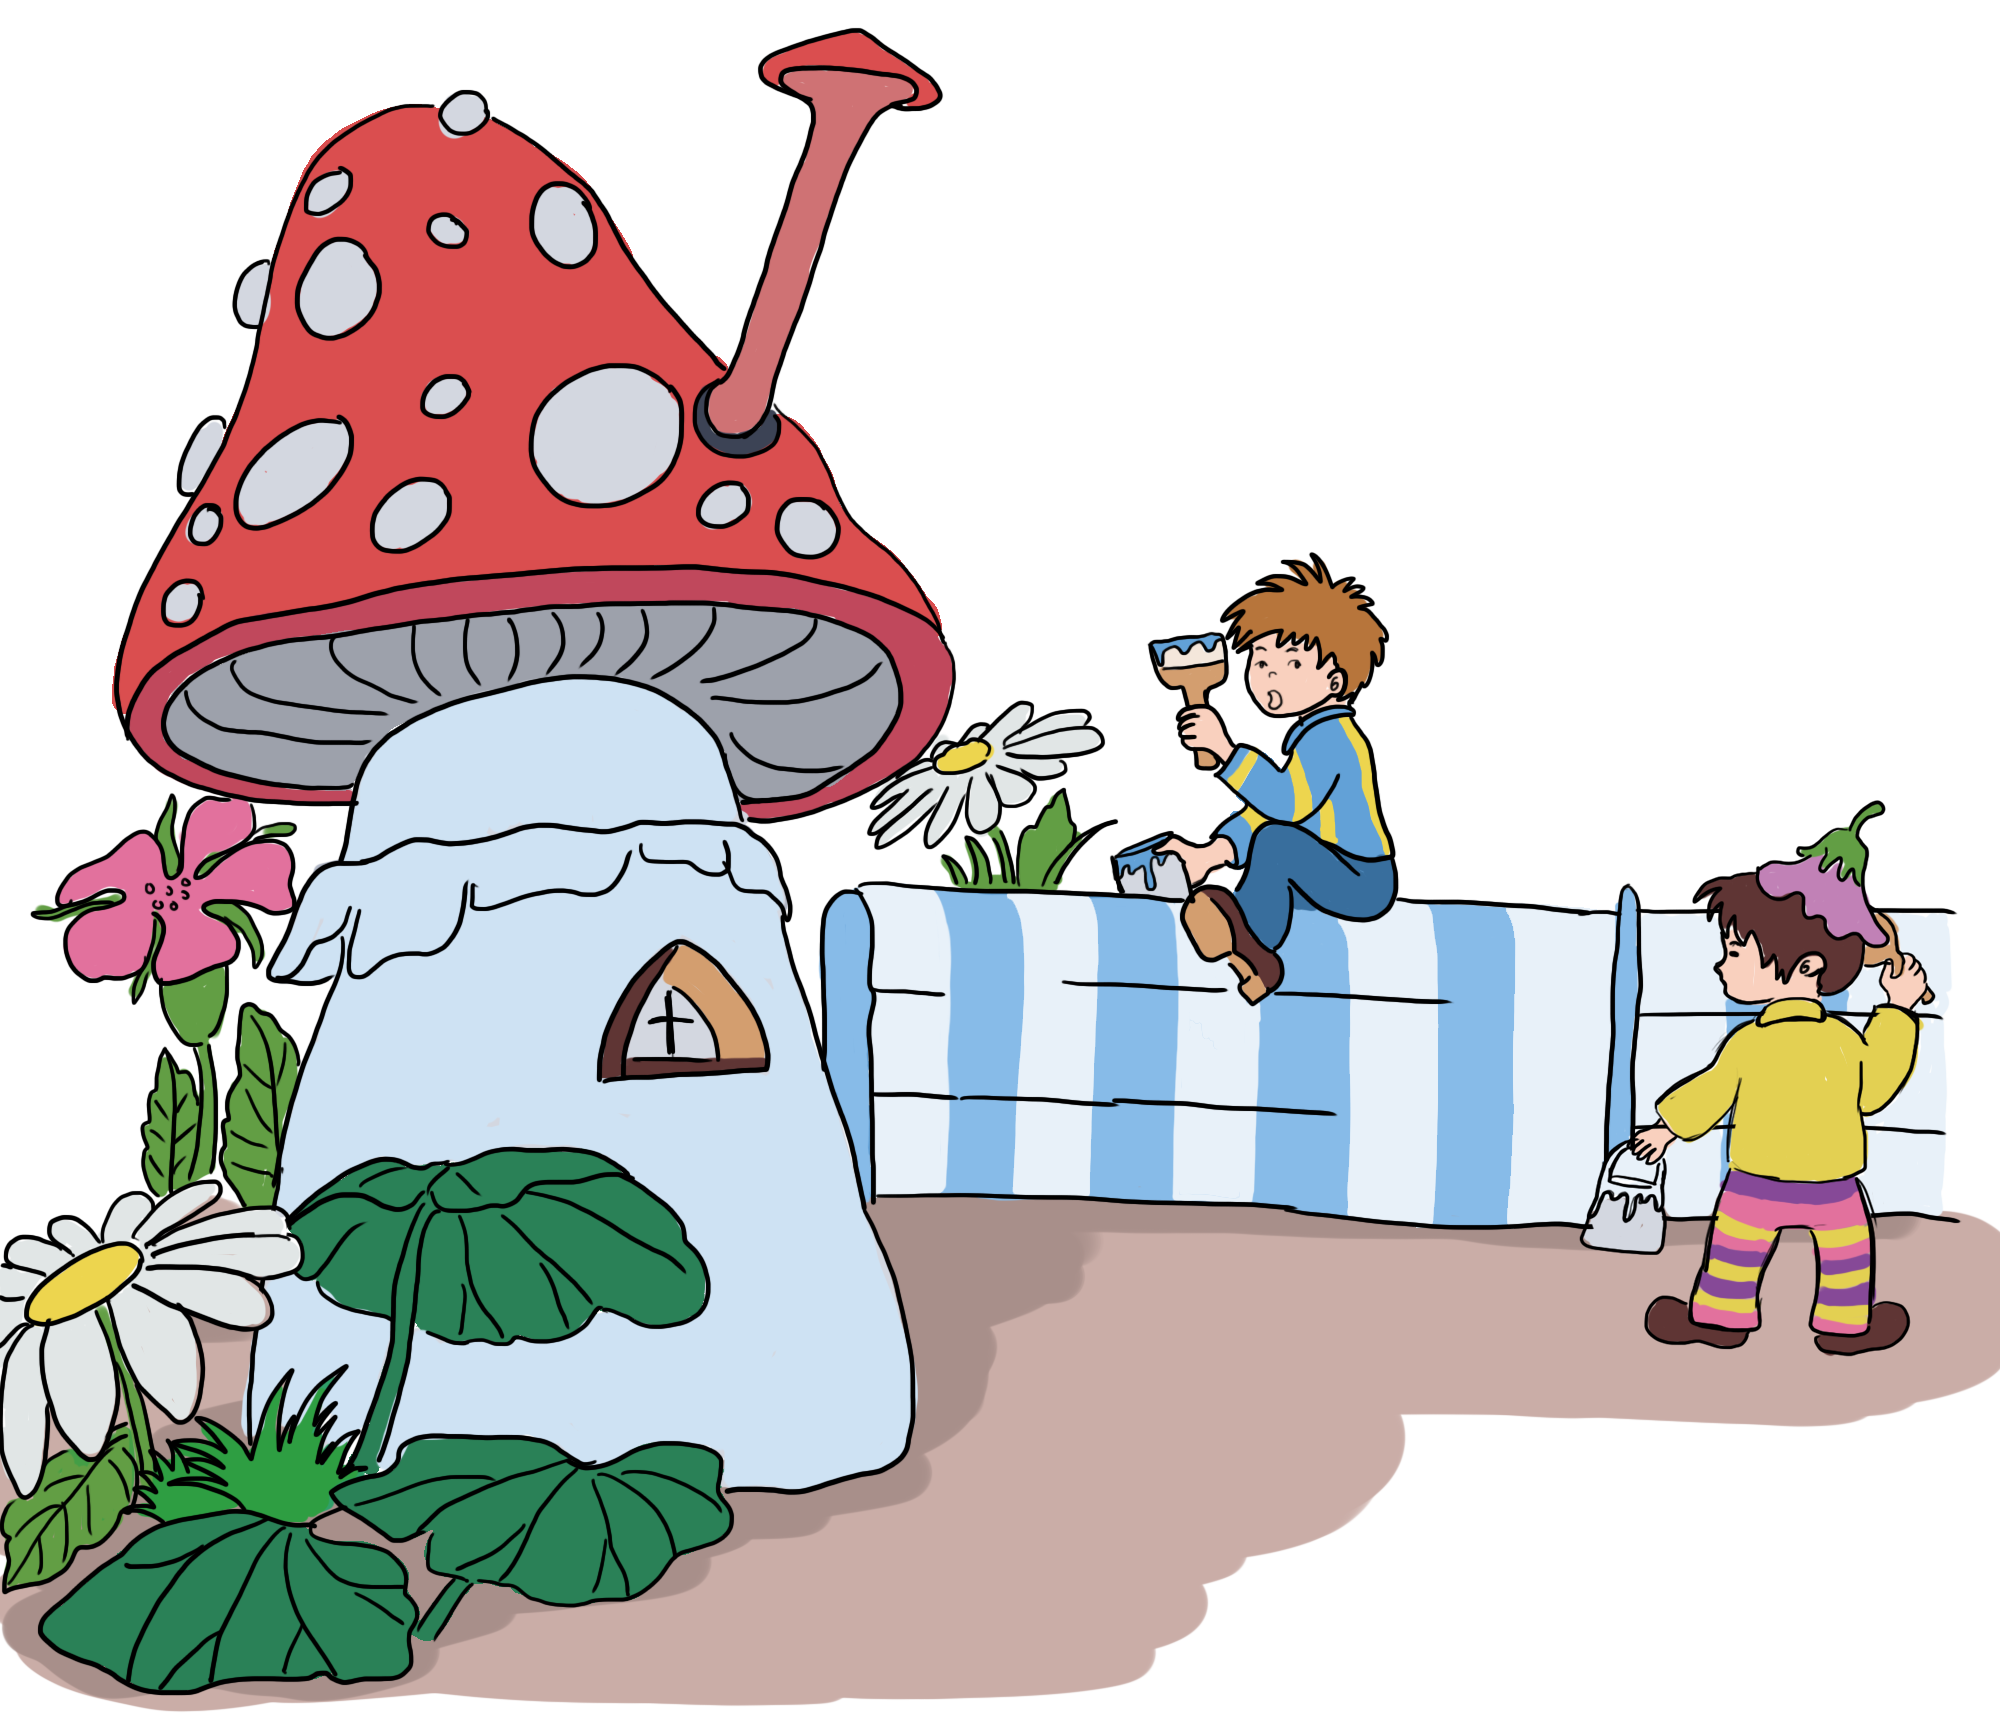
\includegraphics[width=0.55\linewidth]{Hinh14_SonRao}
		%\caption{\textit{\color{toancuabi}Hình $14$.}}
		\vspace*{-10pt}
	\end{figure}
	Quảng trường Cây Táo sắp đón một sự kiện chưa từng có đấy, các bạn đón chờ nhé.
	\vskip 0.1cm
	\centerline{\textbf{\color{toancuabi}Bữa tiệc tại thành phố Xanh}}
	\vskip 0.1cm
	Sau khi bị rơi khỏi Khinh khí cầu, các chú tí hon lạc được đến thành phố Xanh và được các cô tí hon giúp đỡ. Tất nhiên là các chú tí hon cũng giúp các cô rất nhiều việc. Hơn thế nữa, nhờ các chú mà đã hóa giải được hiểu lầm giữa các cô tí hon ở thành phố Xanh và các chú tí hon ở thành phố Diều.  Để kỷ niệm sự kiện này, các cô chú sẽ tổ chức một bữa tiệc long trọng tại quảng trường Cây Táo.
	Các em hãy cùng Mít Đặc tham gia vào bữa tiệc này nhé.
	\vskip 0.1cm
		\begin{wrapfigure}{r}{0.5\linewidth}
		\centering
		\vspace*{5pt}
		\captionsetup{labelformat= empty, justification=centering}
		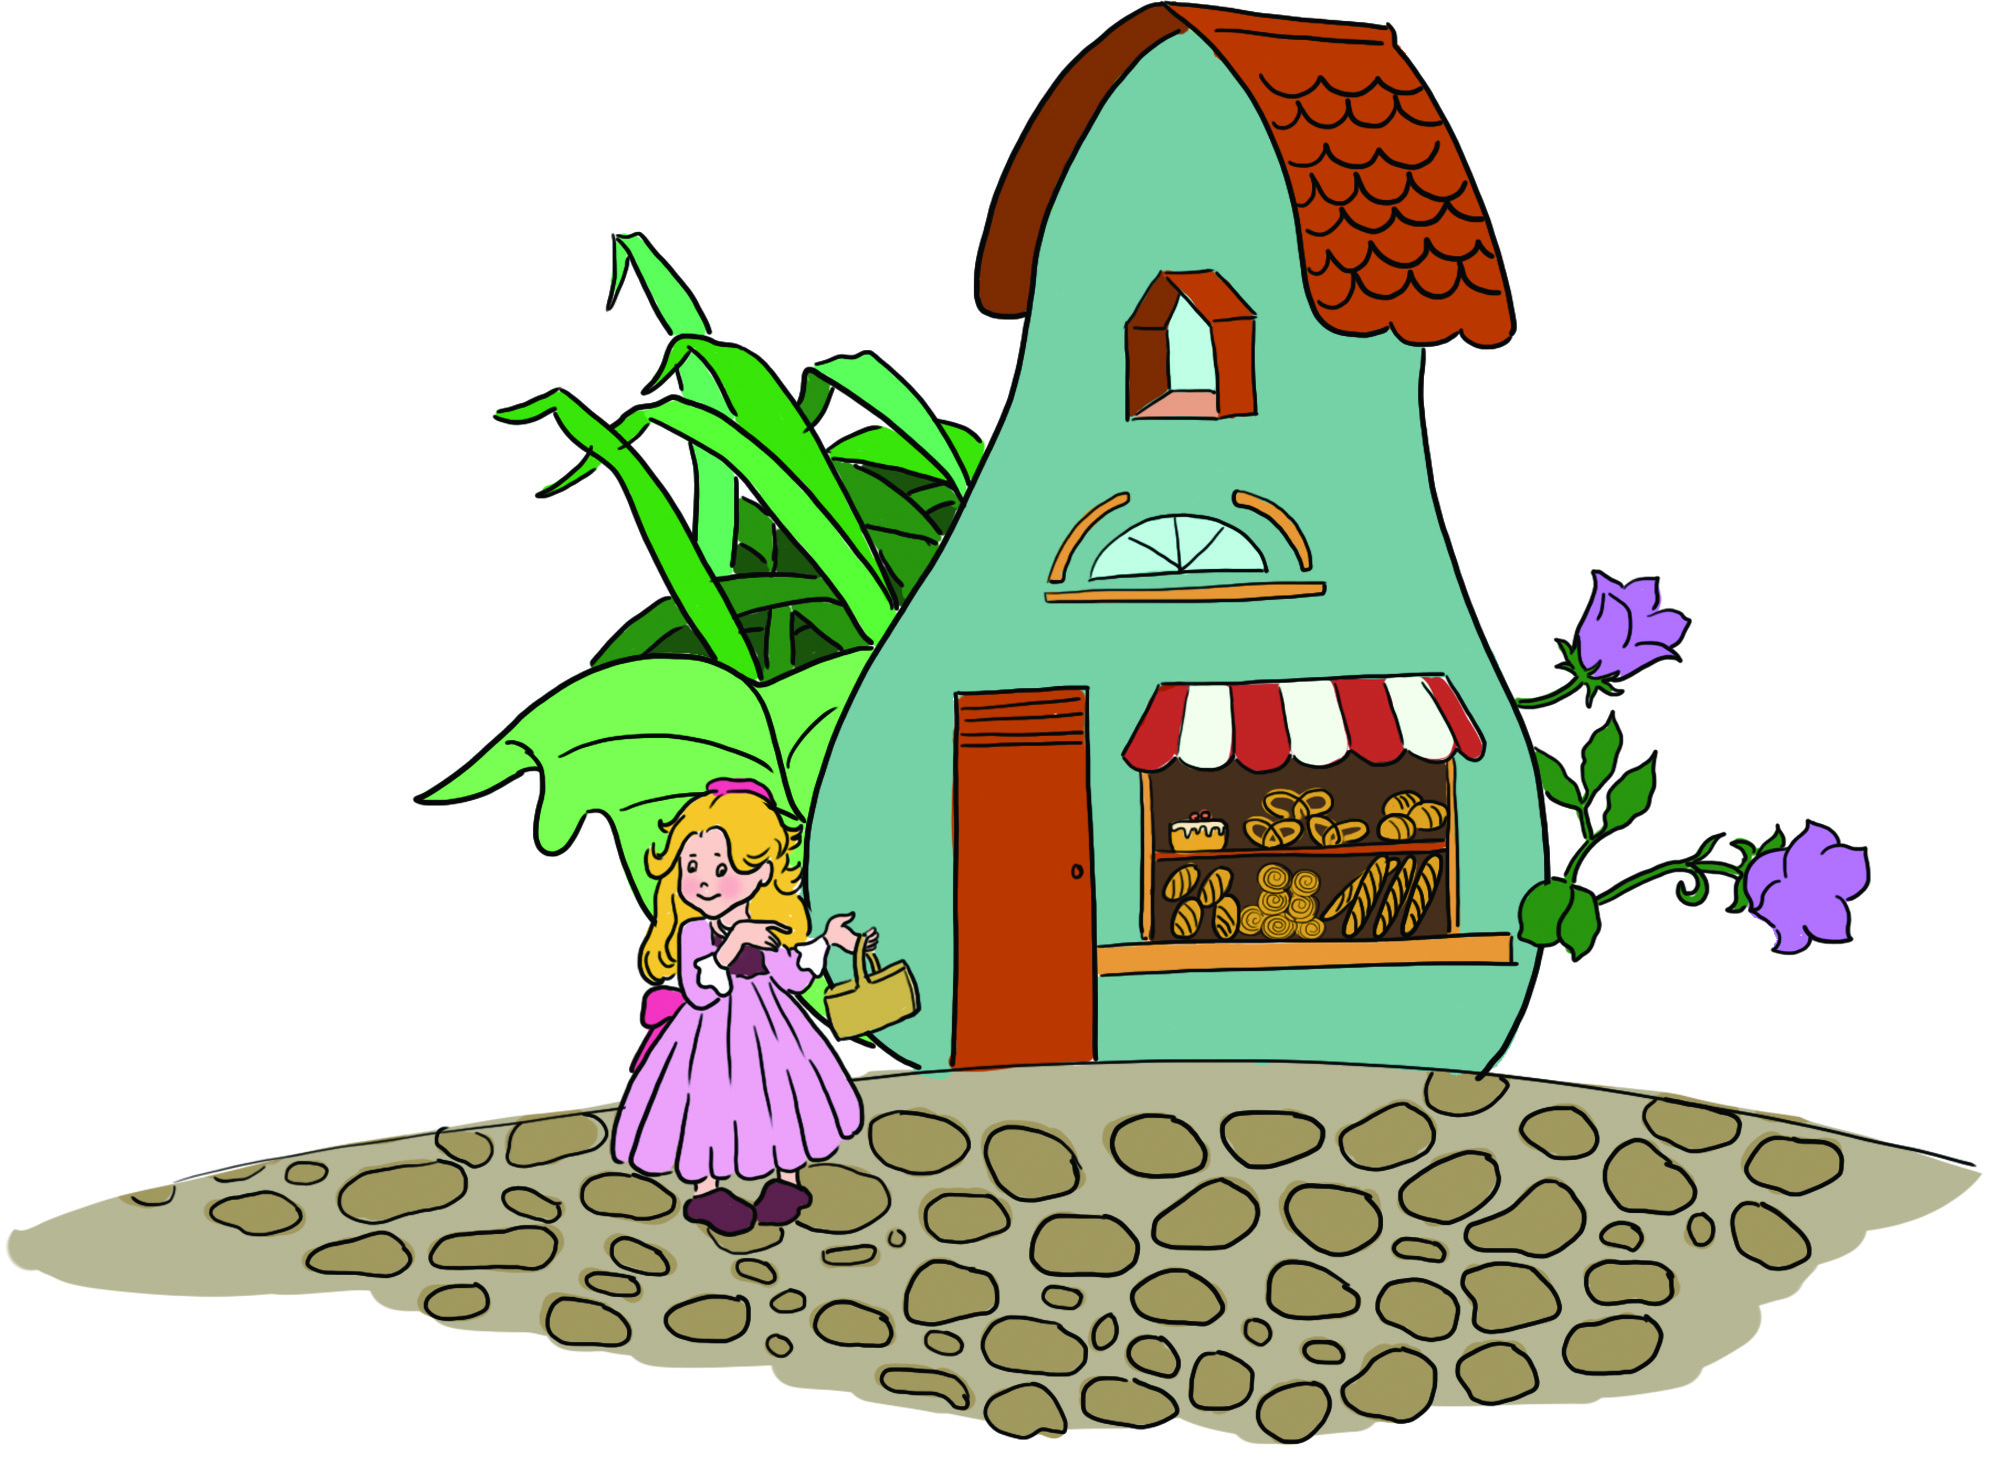
\includegraphics[width=1\linewidth]{Hinh15_BachTuyet}
		%\caption{\textit{\color{toancuabi}Hình $15$.}}
		\vspace*{-15pt}
	\end{wrapfigure}
	\textbf{\color{toancuabi}Câu chuyện $\pmb{13.}$} Tất cả mọi người bắt tay vào việc chuẩn bị cho bữa tiệc. Người thì xén bớt cỏ để làm sân nhảy, người thì dựng lầu để biểu diễn nhạc, xa một chút là một dãy lều dùng để chứa nước ngọt và bánh kẹo. Bạch Tuyết phụ trách việc mua bánh cho bữa tiệc. Cô được giao $100$ đồng để mua và dự định mua hai loại bánh xu kem và bánh gato. Cửa hàng bánh bán $1$ đồng được hai bánh xu kem còn bánh gato giá $13$ đồng một chiếc. Bạch Tuyết có thể mua $100$ chiếc bánh với số tiền đó không các bạn nhỉ?
	\vskip 0.1cm
	\begin{wrapfigure}{l}{0.5\linewidth}
		\centering
		\vspace*{-5pt}
		\captionsetup{labelformat= empty, justification=centering}
		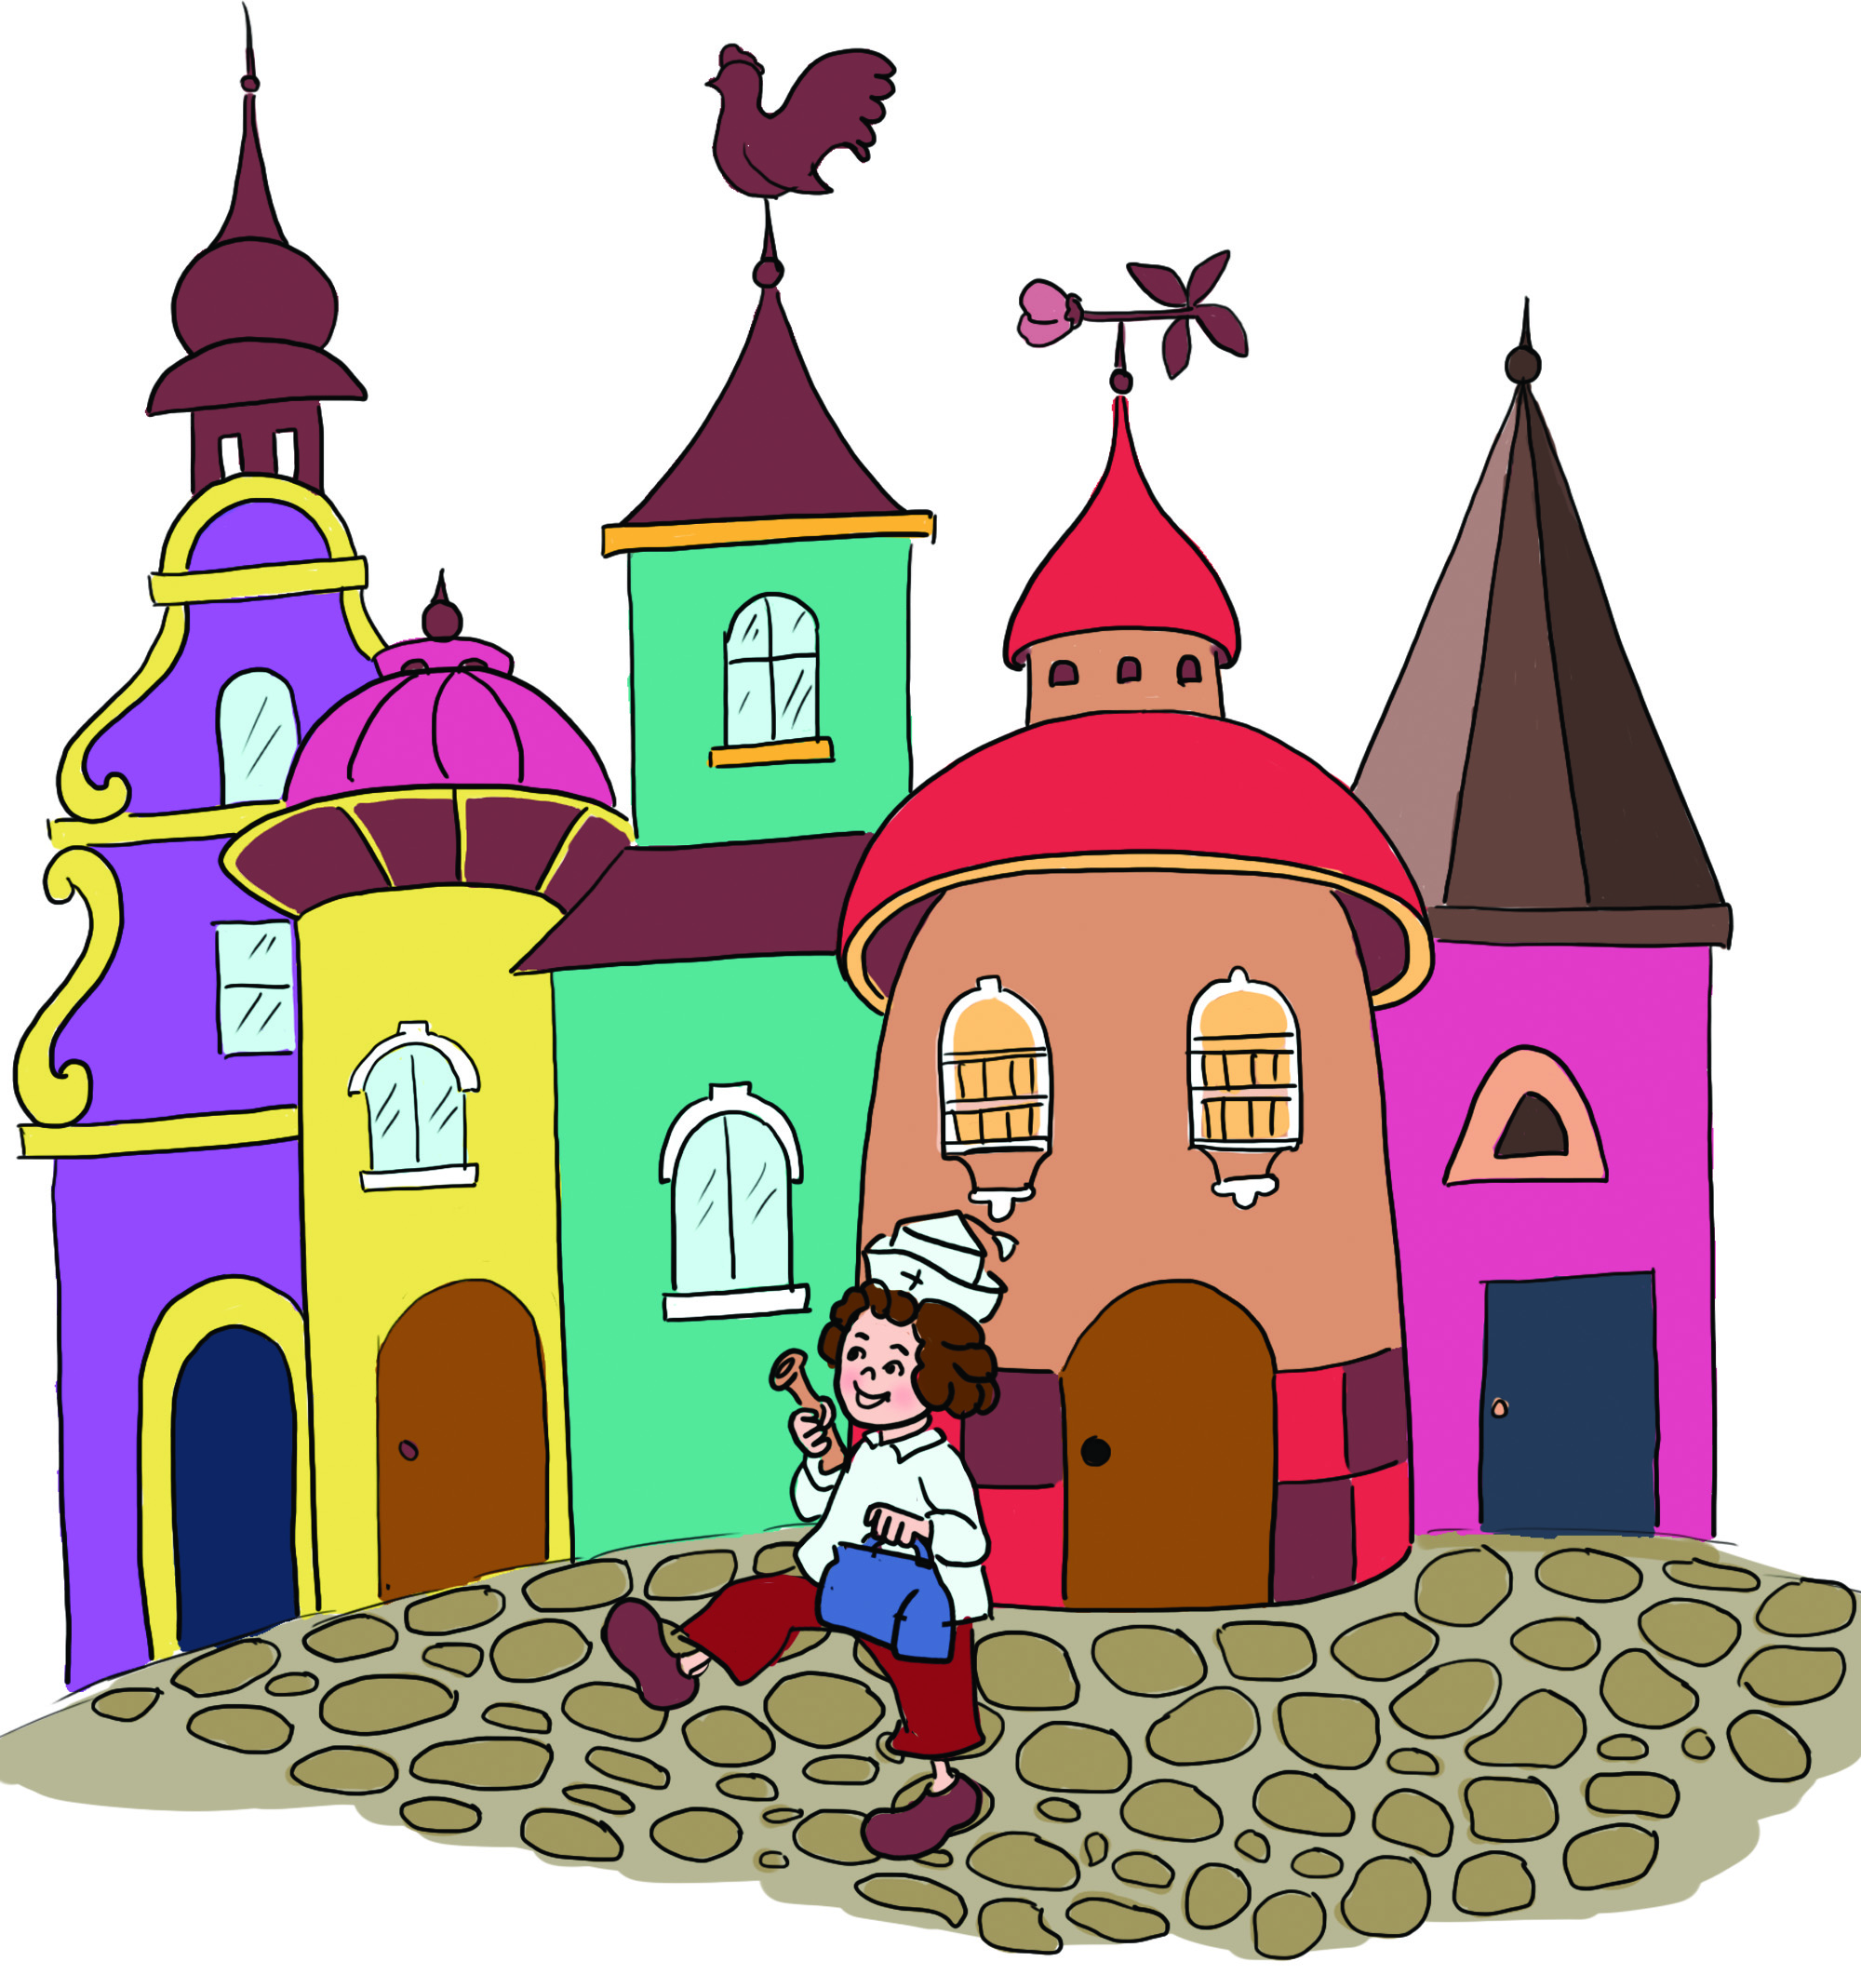
\includegraphics[width=1\linewidth]{Hinh16_ThuocNuoc}
		%\caption{\textit{\color{toancuabi}Hình $16$.}}
		\vspace*{-10pt}
	\end{wrapfigure}
	\textbf{\color{toancuabi}Câu chuyện $\pmb{14.}$} Mặc dù phần lớn các chú tí hon đã ra khỏi bệnh viện, Thuốc Viên vẫn chưa được ra do không nghe lời bác sĩ Mật Ngọt. Cậu tìm cách trốn đến nhà Mít Đặc sớm để đi dự tiệc cùng các bạn. Trên đường, cậu nhẩm tính và tự bảo: nếu giữ nguyên vận tốc thế này thì mình sẽ đến chỗ Mít Đặc $8$ phút trước khi Mít Đặc rời nhà đi dự tiệc. Thật không may, giữa đường cậu nhận ra là mình chưa thay bộ quần áo bệnh viện nên phải quay lại. Vì việc này mà cậu đến chỗ Mít Đặc muộn hơn $10$ phút so với dự định. Hỏi Thuốc Viên đã đi được bao nhiêu phần của quãng đường khi phát hiện ra mình quên thay quần áo, biết rằng tổng thời gian đi của cậu là $38$ phút?
		
	\textbf{\color{toancuabi}Câu chuyện $\pmb{15.}$} Trong bữa tiệc, các chú Tí hon rủ các cô tí hon chơi trò domino, mỗi người tham gia trò chơi sẽ được phát $2$ quân domino. Bạch Tuyết thông báo là có $40$ cô tí hon muốn chơi trò chơi này. Tuy nhiên, bộ domino các chú tí hon mang theo chỉ có $28$ quân, mỗi quân có hai ô, mỗi ô có từ $0$ đến $6$ chấm, và không có hai quân domino nào giống hệt nhau. Mít Đặc đề xuất là sẽ làm bộ domino mới với số chấm thay đổi từ $0$ đến $12$. Các bạn tính thử xem với đề xuất của Mít Đặc thì bộ domino mới có đủ để phát cho $40$ cô tí hon tham gia chơi không nhé.
	\begin{figure}[H]
		\centering
		\vspace*{-5pt}
		\captionsetup{labelformat= empty, justification=centering}
		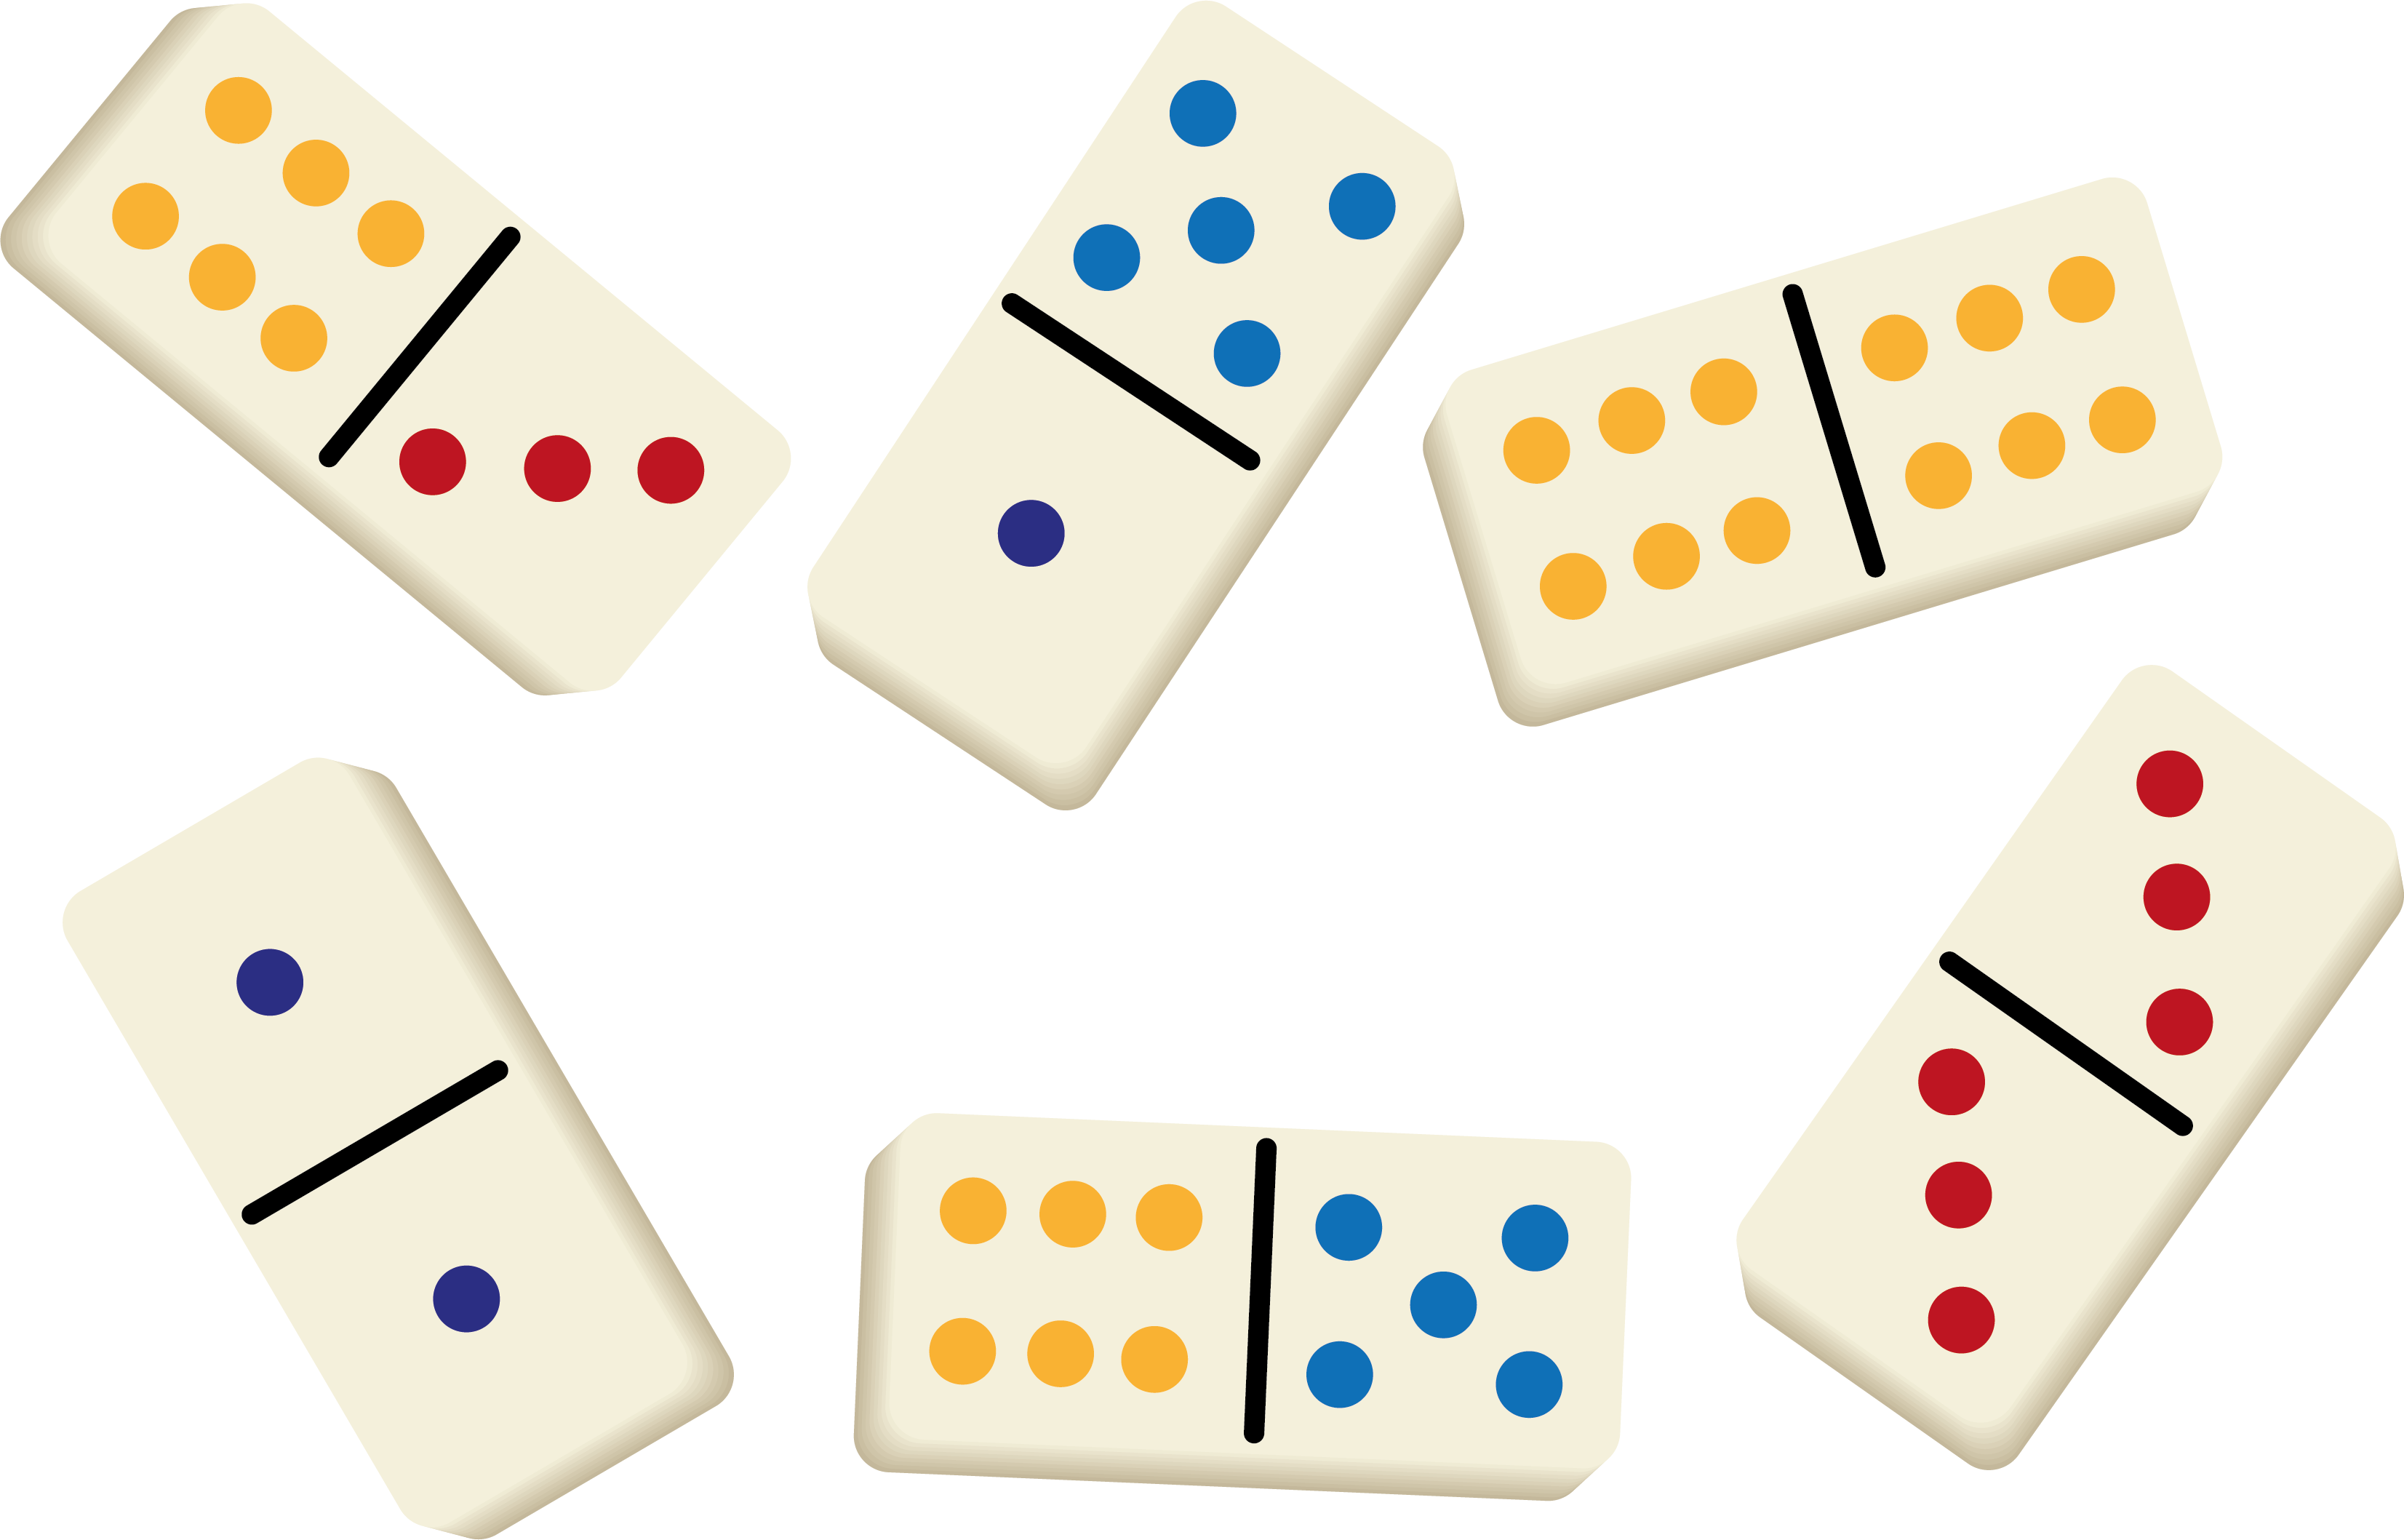
\includegraphics[width=0.6\linewidth]{Hinh17_Domino}
		%\caption{\textit{\color{toancuabi}Hình $17$.}}
		\vspace*{-10pt}
	\end{figure}
	\textbf{\color{toancuabi}Câu chuyện $\pmb{16.}$} Cuối buổi tiệc, khách khứa đều được tặng những hộp kẹo đem về. Nhanh Nhảu đề nghị một trò chơi: Đầu tiên cậu ấy sẽ cho Mít Đặc gấp đôi số kẹo mà Mít Đặc có, sau đó lại lấy lại $8$ chiếc. Mít Đặc nghĩ một lúc, thấy có vẻ hời nên đồng ý. Sau $3$ lần trao đổi như thế Mít Đặc thấy trong hộp của mình không còn chiếc kẹo nào. Thật là tai hại! Các bạn tính xem lúc đầu Mít Đặc có bao nhiêu chiếc kẹo nhé.
	\begin{figure}[H]
		\centering
		\vspace*{-5pt}
		\captionsetup{labelformat= empty, justification=centering}
		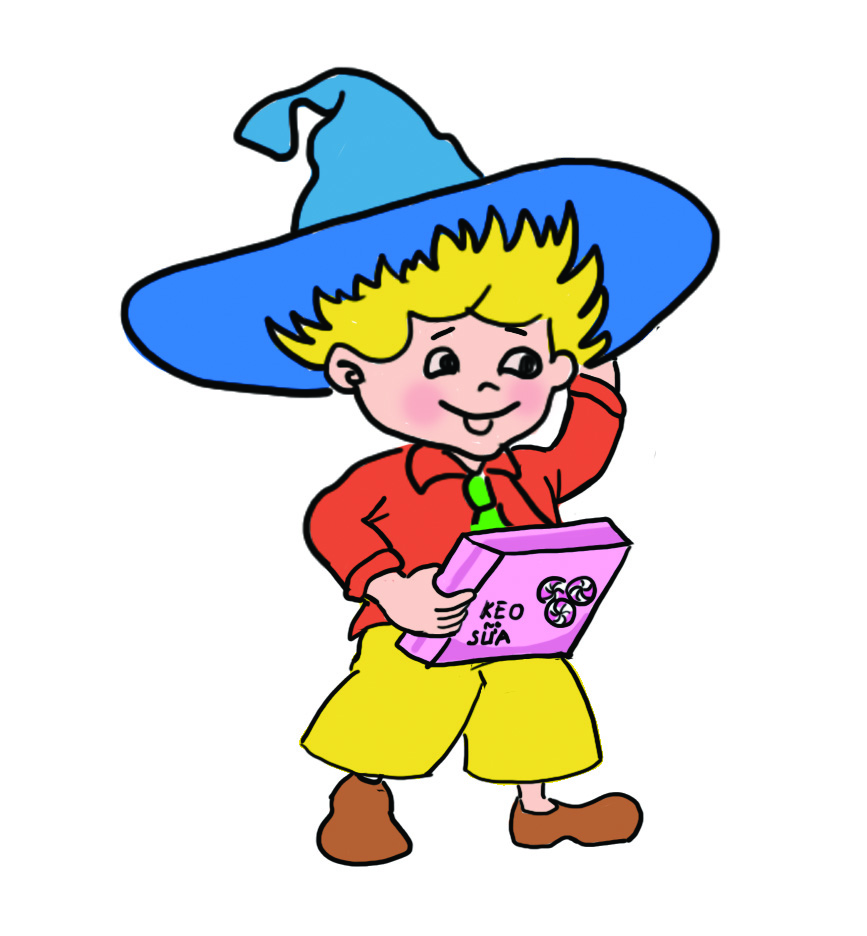
\includegraphics[width=0.4\linewidth]{Hinh18_MitDac}
		%\caption{\textit{\color{toancuabi}Hình $18$.}}
		\vspace*{-10pt}
	\end{figure}
	\centerline{\textbf{\color{toancuabi}Tạm biệt thành phố Xanh}}
	\vskip 0.1cm
	\begin{multicols}{2}
		\textit{Sau một thời gian lưu trú tại thành phố Xanh, các chú tí hon đã quyết định trở về thành phố Hoa của mình. Các cô chú tí hon đã rất buồn khi phải tạm biệt nhau. Để lưu thành những kỷ niệm, nhiều hoạt động đã diễn ra: Kèn Đồng sáng tác nhạc và Hoa Dại làm thơ tặng các bạn mình, các cô tí hon đã may túi tặng các chú tí hon rồi các cô chú cùng nhau tổ chức một buổi vũ hội,\ldots Các bạn nhỏ hãy cùng các cô chú tí hon tham gia vào các hoạt động này qua các bài toán dưới đây nhé.}
		\begin{figure}[H]
			\centering
			\vspace*{-5pt}
			\captionsetup{labelformat= empty, justification=centering}
			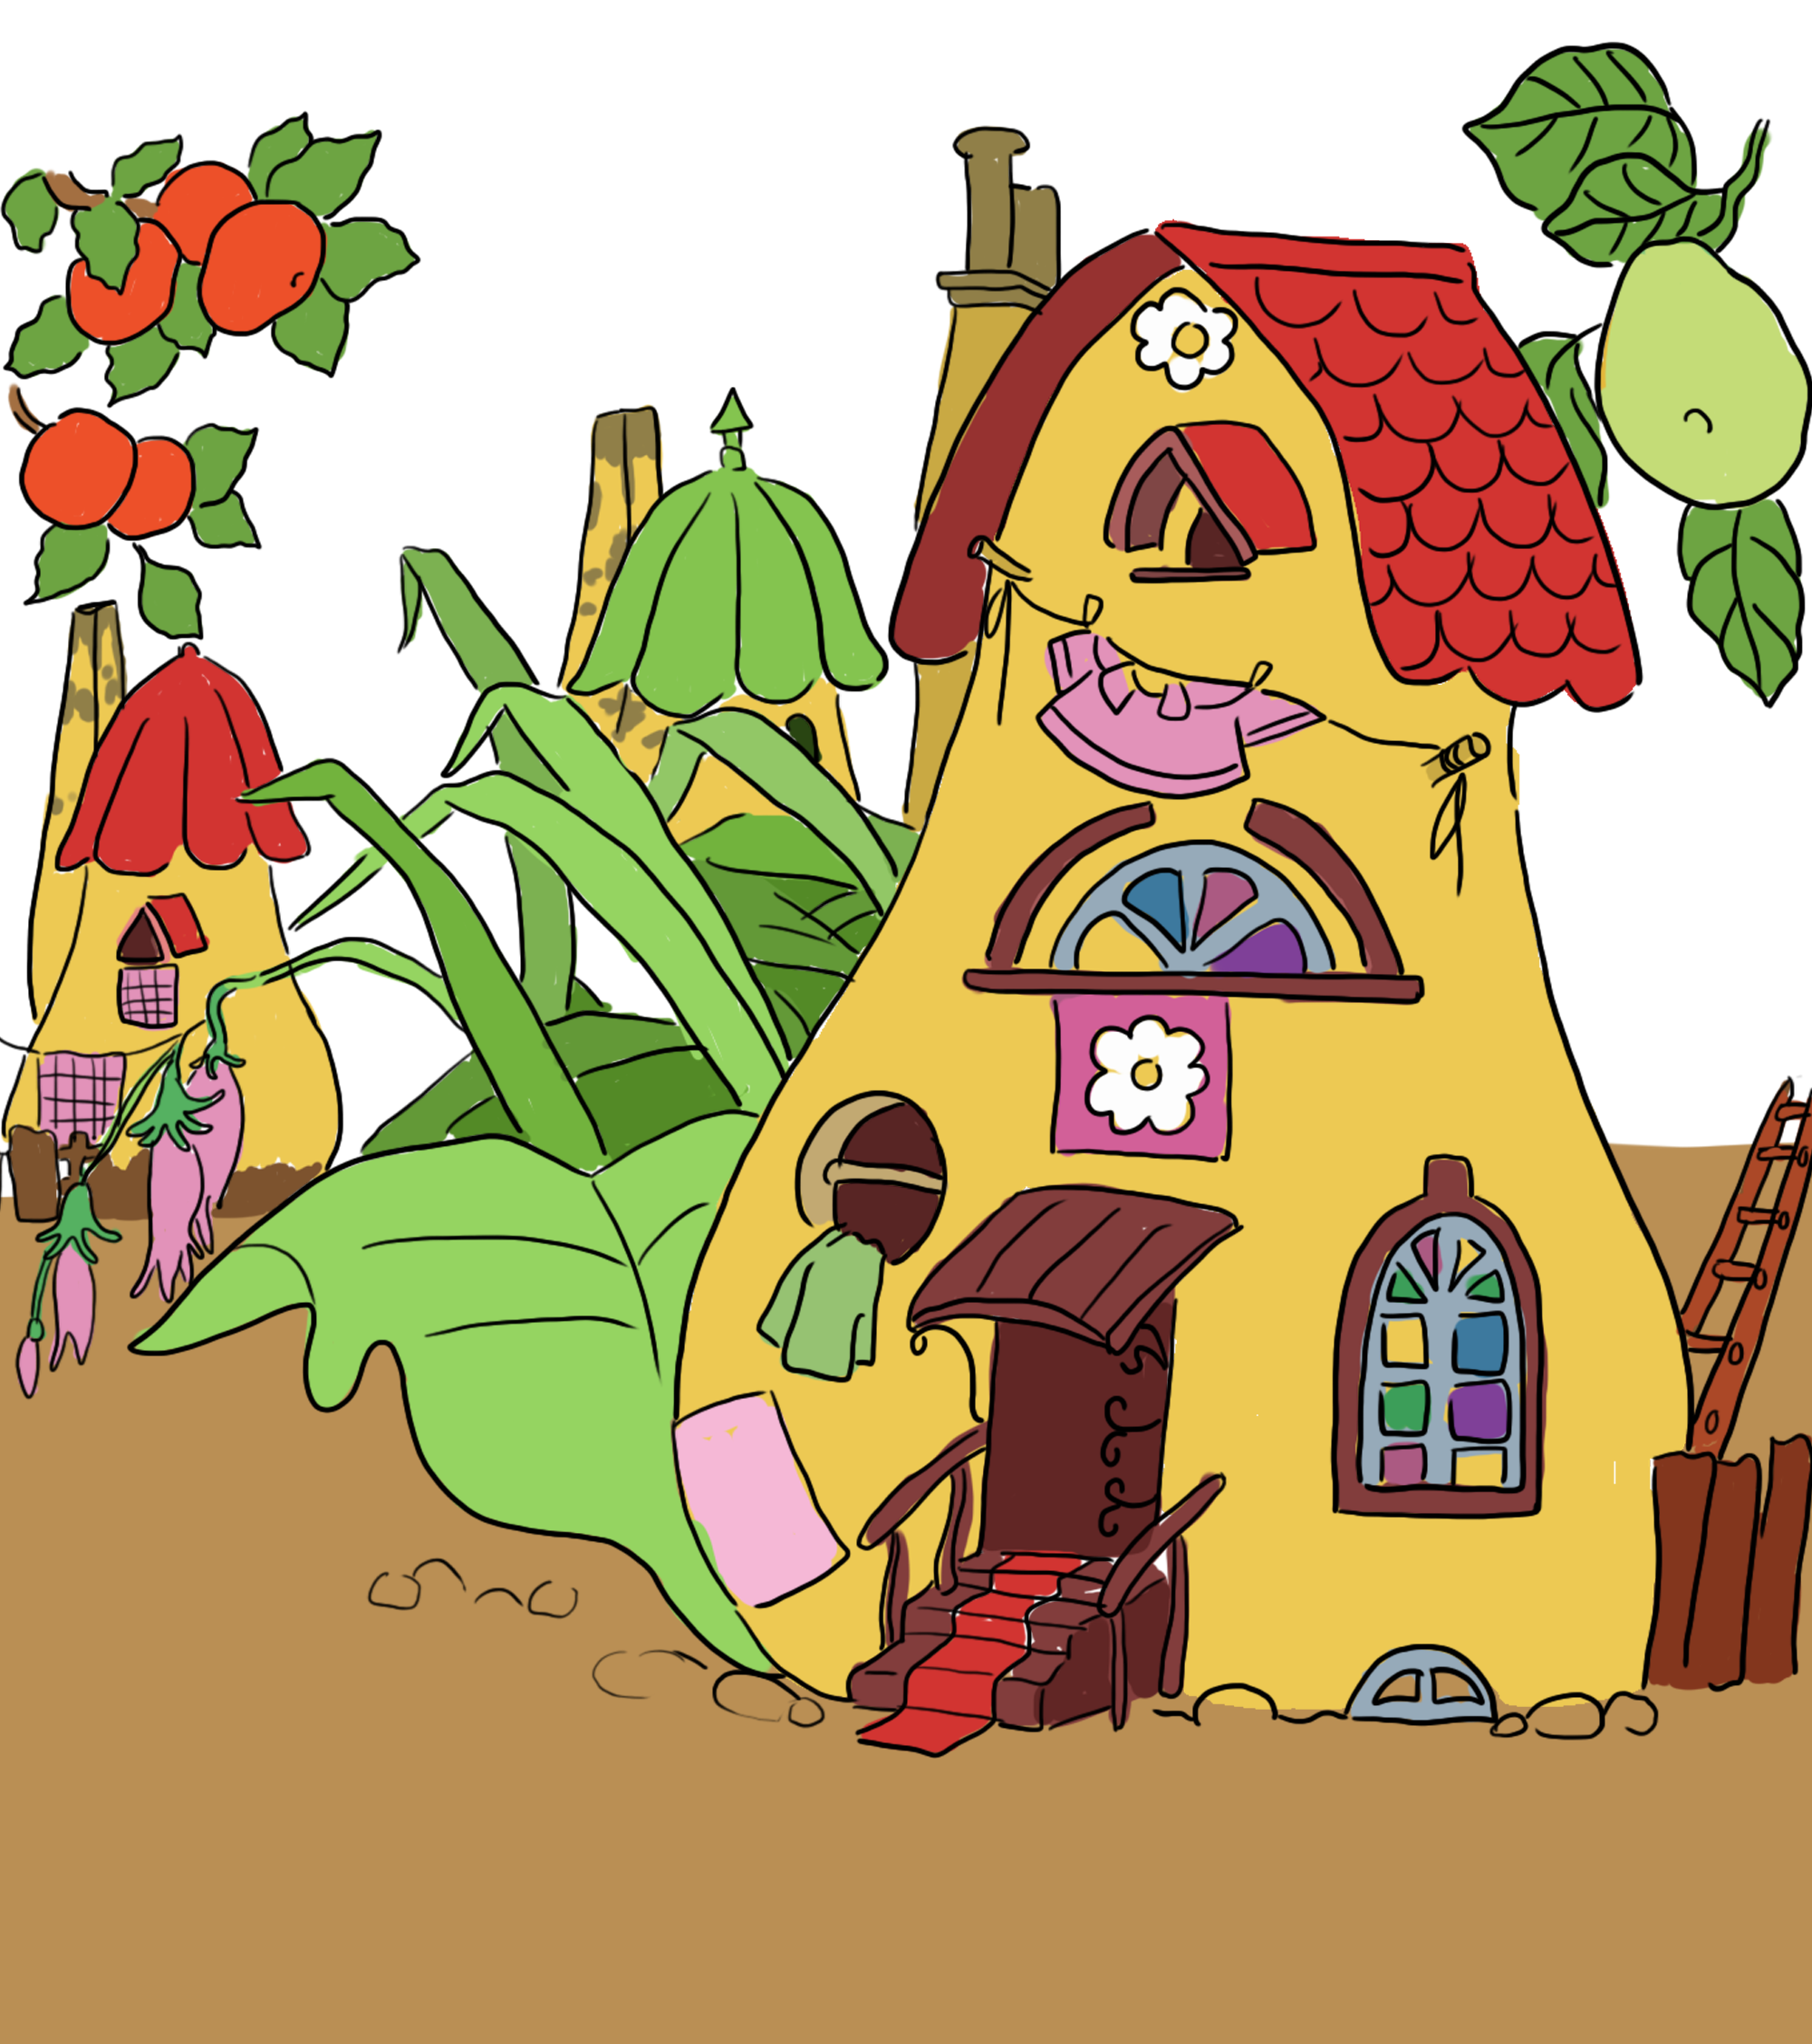
\includegraphics[width=1\linewidth]{Hinh10_ThanhPhoXanh}
			%\caption{\textit{\color{toancuabi}Hình $18$.}}
			\vspace*{-10pt}
		\end{figure}
	\end{multicols}
	\vskip 0.1cm
		\begin{wrapfigure}{l}{0.5\linewidth}
		\centering
		\vspace*{-5pt}
		\captionsetup{labelformat= empty, justification=centering}
		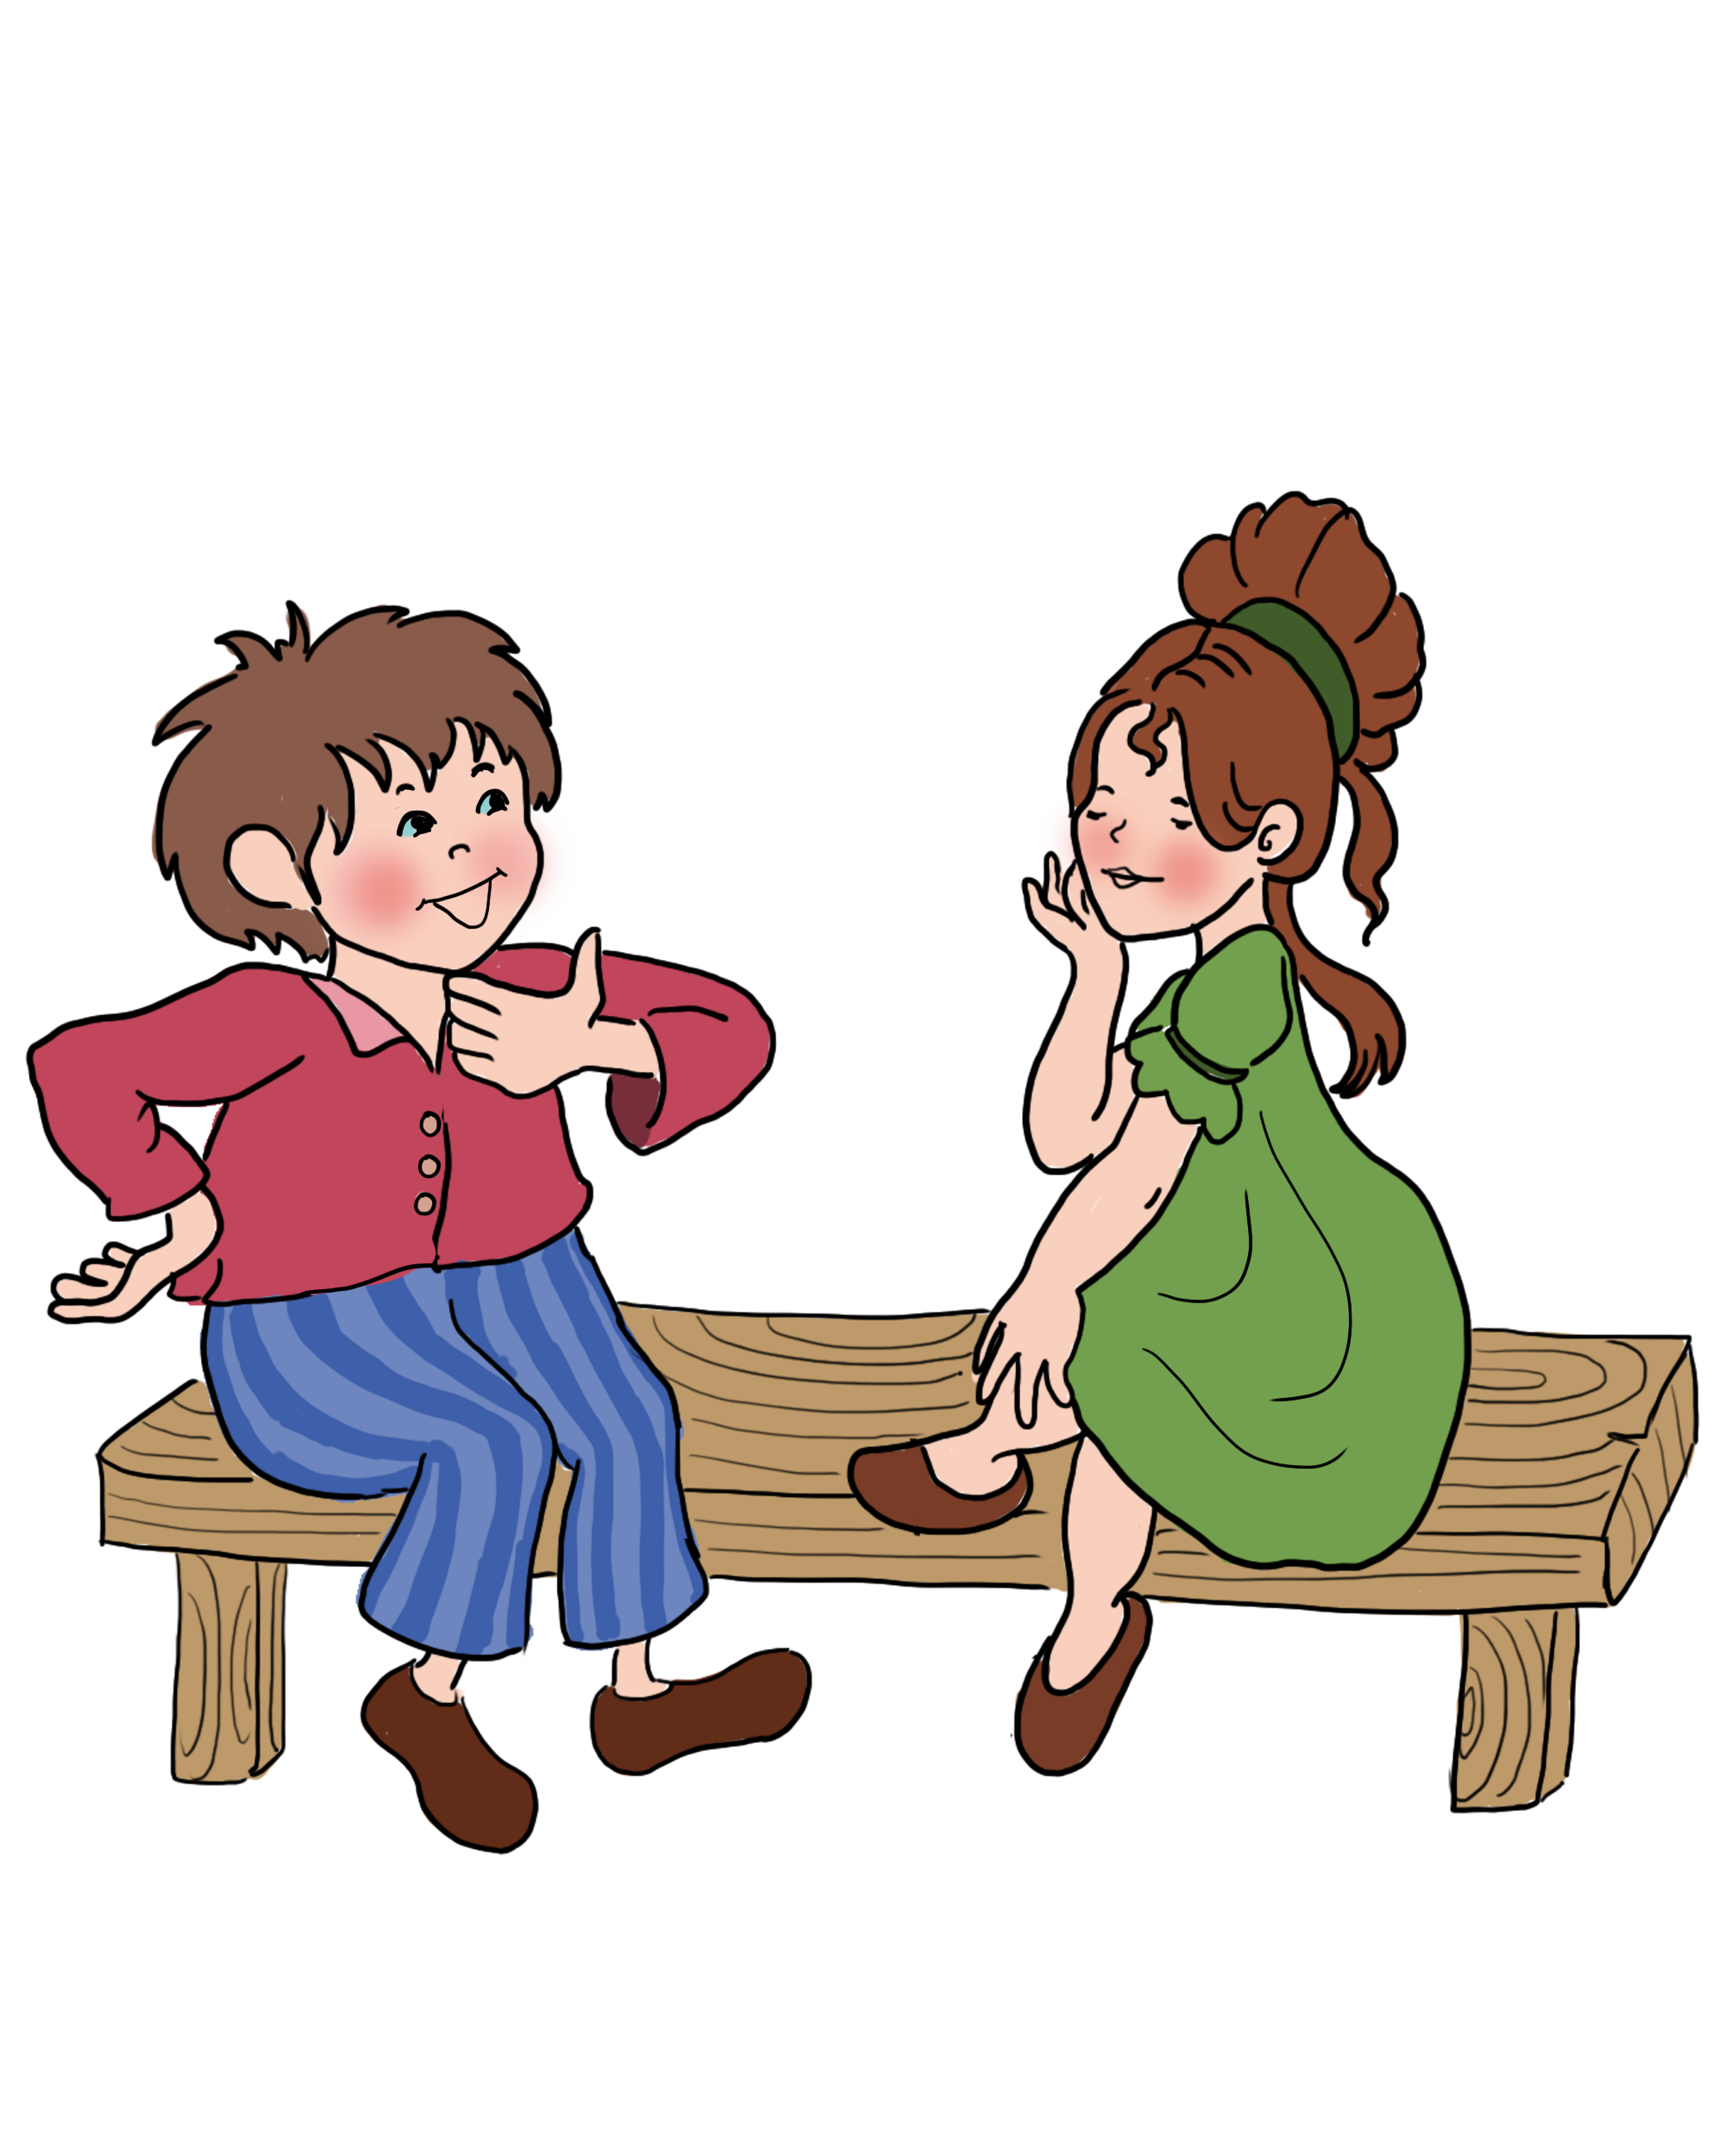
\includegraphics[width=1\linewidth]{Hinh19_KenDong_HoaGiay}
		\vspace*{-15pt}
	\end{wrapfigure}
	\textbf{\color{toancuabi}Câu chuyện $\pmb{17.}$} Sắp đến thời gian các chú tí hon phải trở về thành phố Hoa, nhạc sĩ Kèn Đồng sáng tác một bài hát và thi sĩ Hoa Dại làm một bài thơ tặng các bạn của mình. Vì nóng lòng muốn khoe ngay tác phẩm mình vừa sáng tác, sáng sớm hôm sau, hai bạn cùng đi sớm nhất có thể (thế nên cùng thời điểm) để đến nhà nhau. Vì mải hát và ngâm thơ dọc đường nên hai bạn không nhìn thấy nhau tại lúc gặp nhau giữa đường. Sau thời điểm gặp, Hoa Dại đến nhà Kèn Đồng sau đó $4$ phút, còn Kèn Đồng đến nhà Hoa Dại sau đó $1$ phút. Các bạn hãy tính xem mỗi thi sĩ đã đi đến nhà nhau mất bao nhiêu phút nhé.
	\newpage
	\begin{wrapfigure}{l}{0.5\linewidth}
		\centering
		\vspace*{5pt}
		\captionsetup{labelformat= empty, justification=centering}
		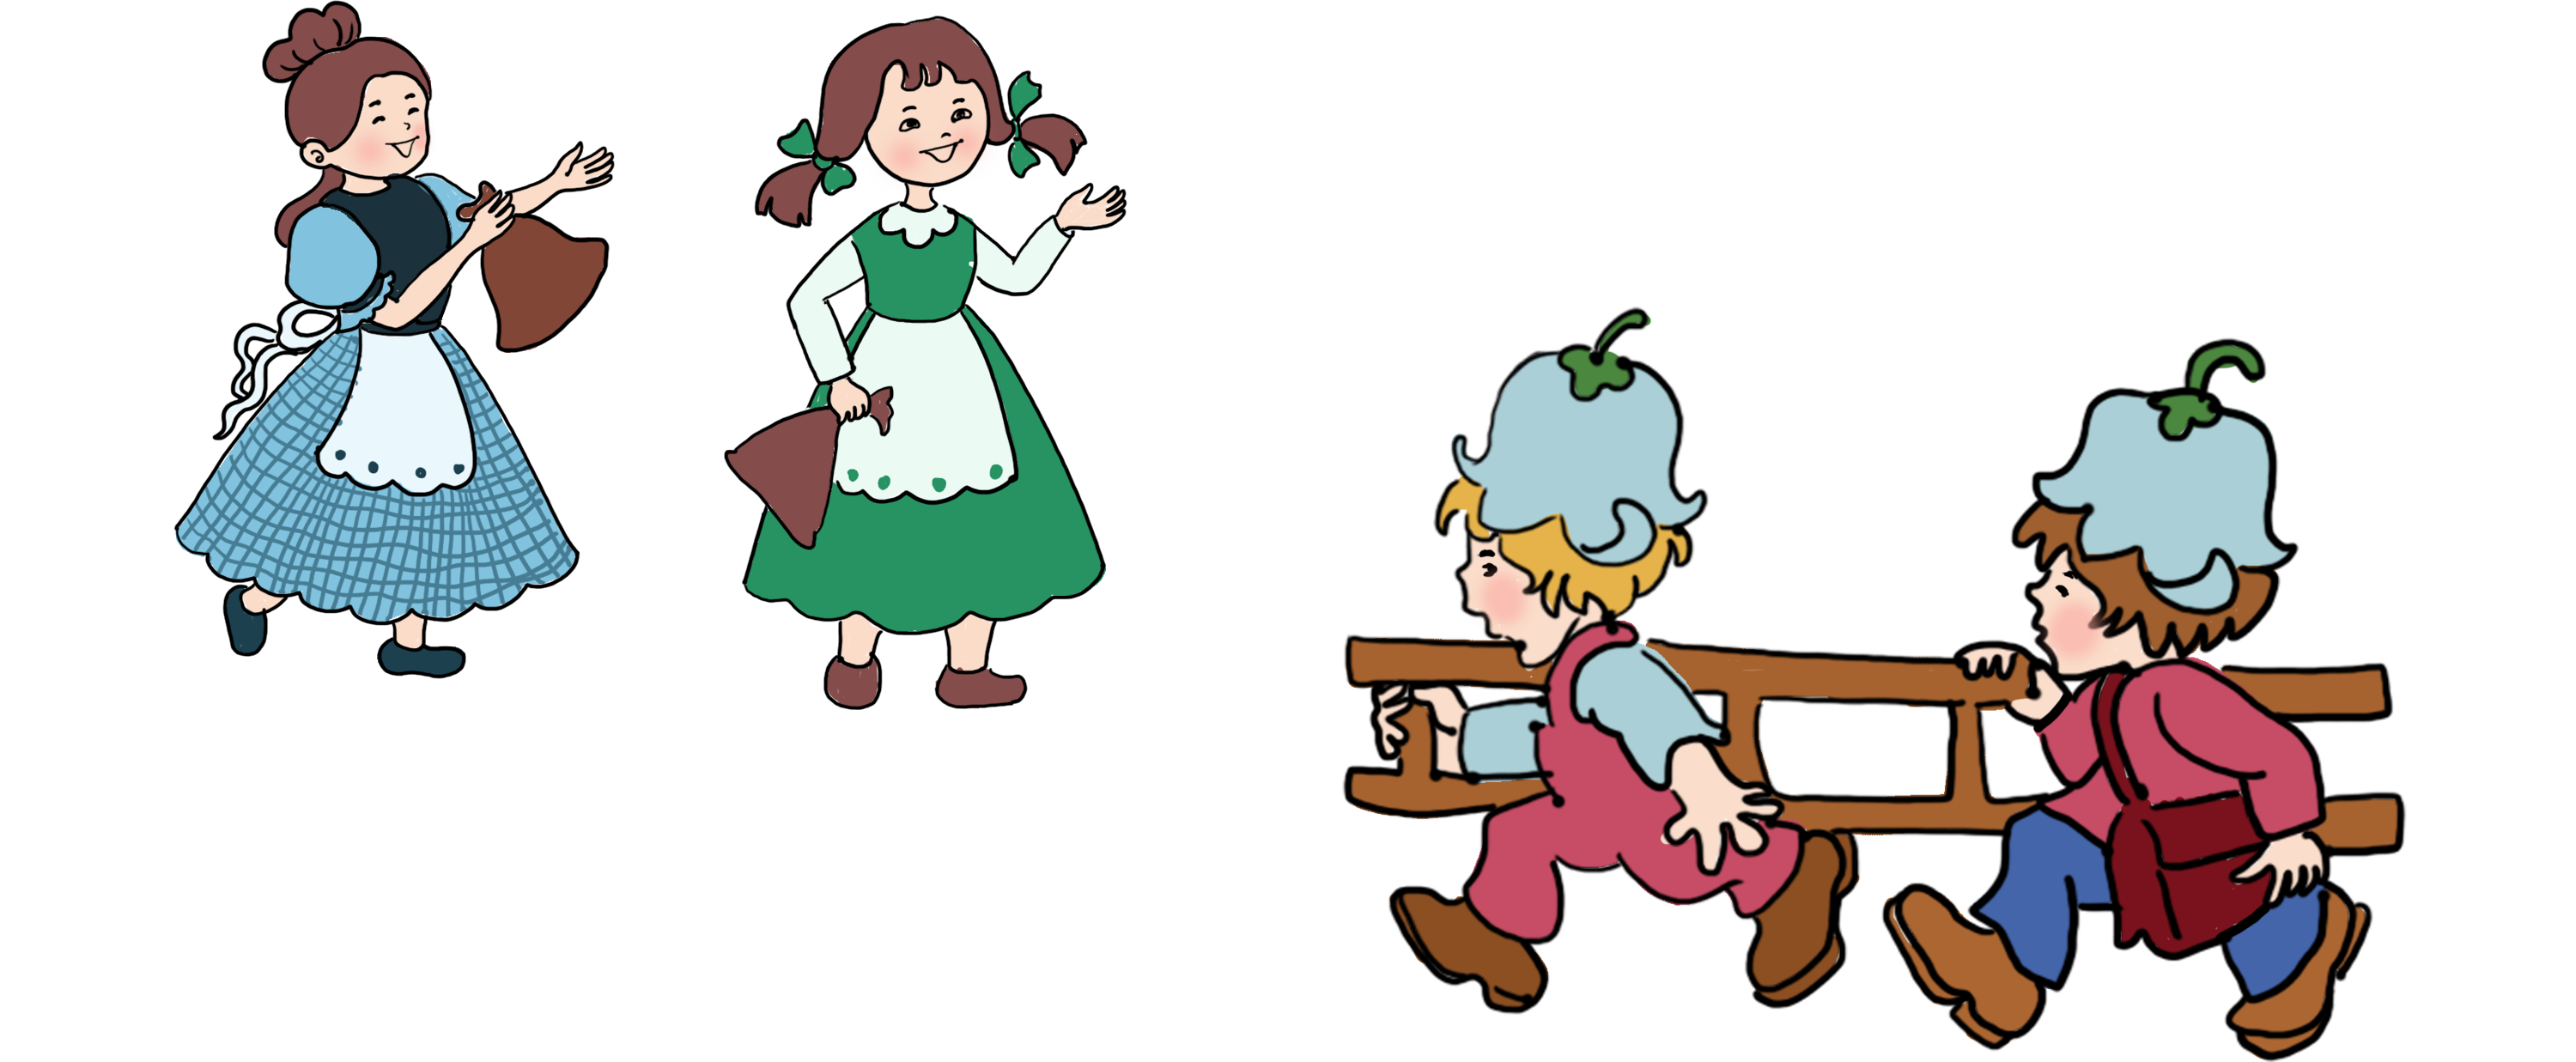
\includegraphics[width=1\linewidth]{Hinh20_TangTui}
		%\caption{\textit{\color{toancuabi}Hình $20$.}}
		\vspace*{-10pt}
	\end{wrapfigure}
	\textbf{\color{toancuabi}Câu chuyện $\pmb{18.}$} Để làm kỷ niệm, Mắt Xanh và một số cô tí hon trong thành phố Xanh đã may túi tặng các chú tí hon. Mỗi cô trong nhóm đã may được một số lượng túi như nhau và cùng nhau mang túi đến tập hợp ở nhà Bạch Tuyết. Trên đường đi, các cô gặp một nhóm các chú tí hon và thật trùng họp số chú tí hon trong nhóm đúng bằng số các cô tí hon, mỗi cô đã tặng mỗi chú tí hon một chiếc túi mà mình may được. Sau khi tặng túi, mỗi cô tí hon vẫn còn hơn $1$ chiếc và tập hợp tất cả lại được $33$ chiếc mang đến nhà Bạch Tuyết. Các bạn có tính được mỗi cô tí hon đã may bao nhiêu chiếc túi không?
	\vskip 0.1cm
	\begin{wrapfigure}{r}{0.5\linewidth}
		\centering
		\vspace*{-5pt}
		\captionsetup{labelformat= empty, justification=centering}
		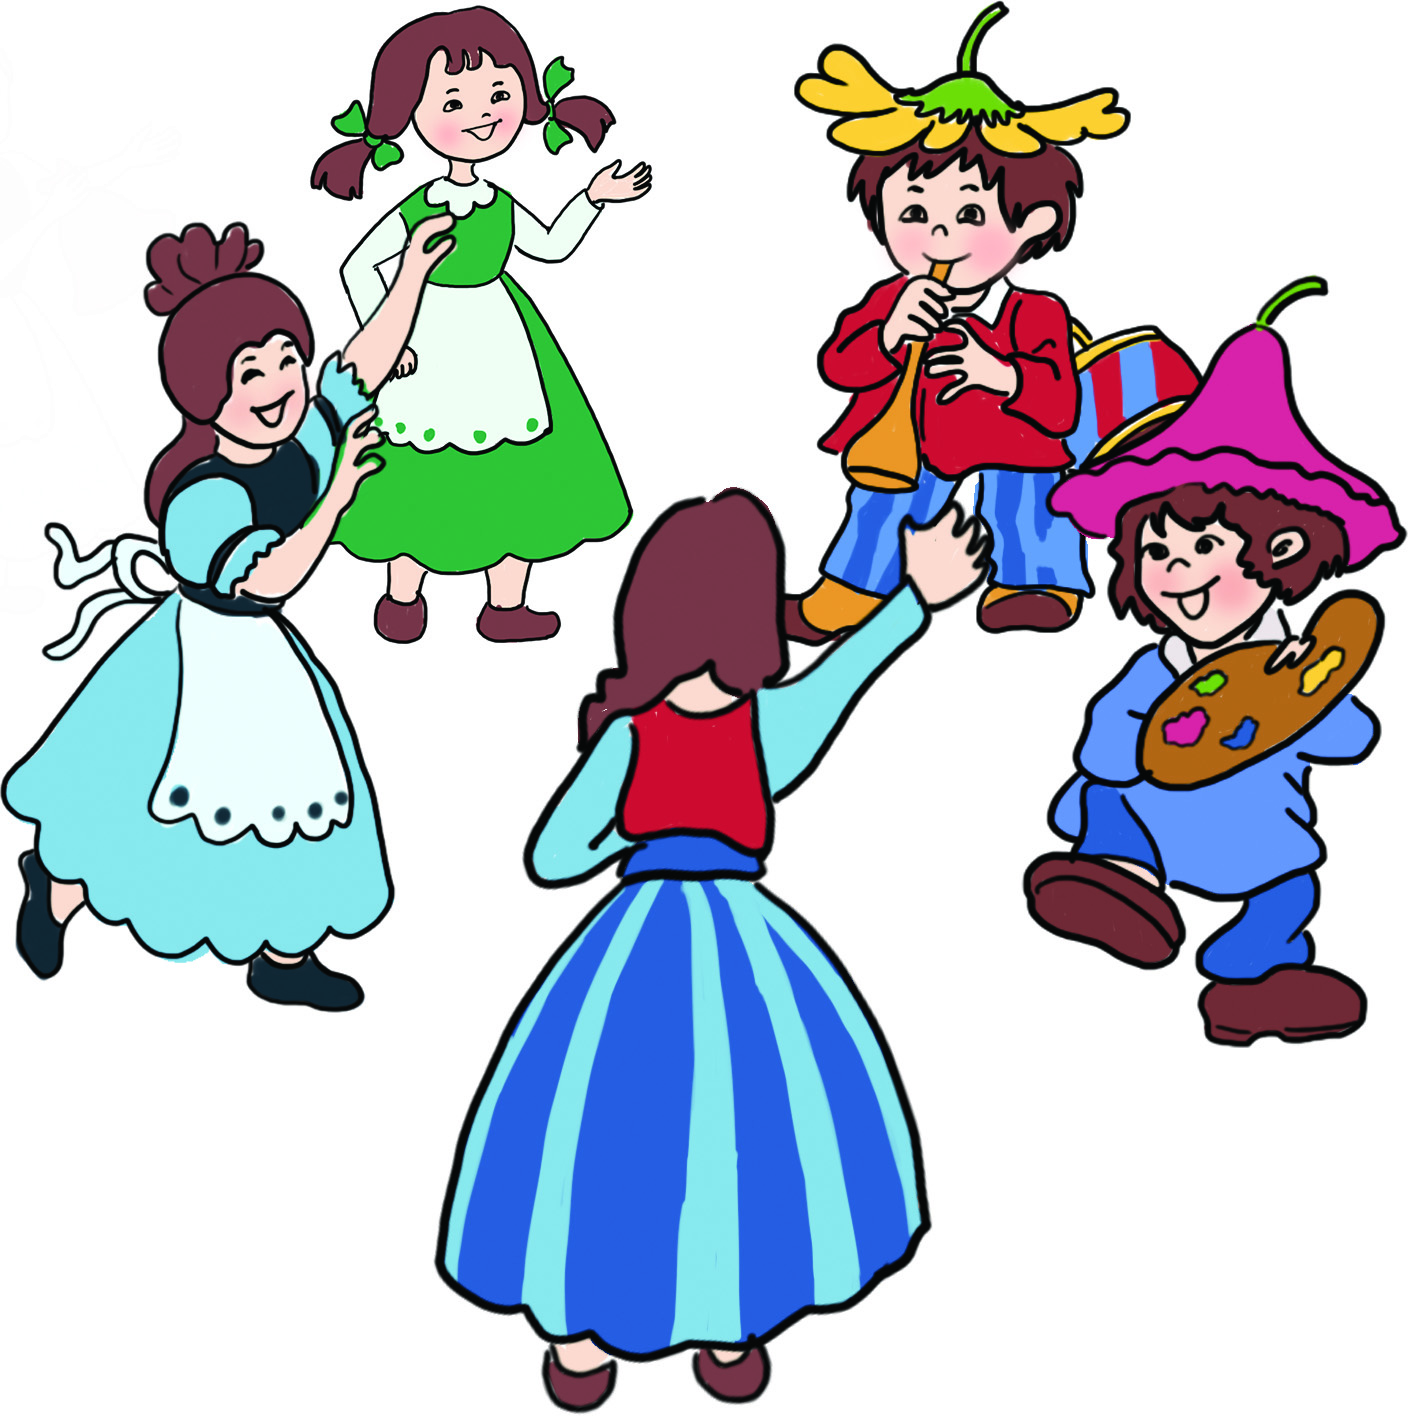
\includegraphics[width=1\linewidth]{Hinh21_VongTron}
		\vspace*{-15pt}
	\end{wrapfigure}	
	\textbf{\color{toancuabi}Câu chuyện $\pmb{19.}$} Một buổi vũ hội đã được tổ chức trước ngày các chú tí hon trở về. Cuối buổi, các cô chú tí hon xếp thành một vòng tròn để nghe hai Kèn Đồng biểu diễn nhạc và Hoa Dại đọc thơ. Mít Đặt và Tròn Xoay mải chạy loanh quanh nên không kịp tham gia vào vòng tròn này. Tròn Xoay nói: “Tớ chưa từng thấy nhiều người trong một vòng tròn như thế. Chúng ta đếm thử xem có bao nhiêu người nhé.” Mít Đặc và Tròn Xoay cùng đi theo một chiều để đếm số người trong vòng tròn nhưng bắt đầu từ những người khác nhau. Người thứ $20$ theo cách đếm của Mít Đặc lại là người thứ $7$ theo cách đếm của Tròn Xoay, còn người thứ $7$ theo cách của đếm của Mít Đặc lại là người thứ $94$ theo cách của Tròn Xoay. Thế thì vòng tròn này có bao nhiêu cô chú tí hon nhỉ? Các bạn có tính được không?
	\vskip 0.1cm
	\textbf{\color{toancuabi}Câu chuyện $\pmb{20.}$} Khi chia tay với các cô tí hon, Mít Đặc hứa là sẽ viết thư cho Mắt Xanh, thế nên từ khi trở về thành phố Hoa, cậu chịu khó luyện viết lắm, dạo này cậu còn học thêm cả toán nữa. Trong bức thư trước, Mắt Xanh hỏi bao giờ thì các chú làm xong kinh khí cầu để quay lại thăm thành phố Xanh. Trong bức thư lần này gửi cho Mắt Xanh, Mít Đặc được dịp thể hiện luôn, cậu viết: “Chúng tớ đang làm kinh khí cầu rồi. Biết Tuốt đã dự tính một số ngày. Nếu mỗi người bọn tớ làm $6$ ngày công thì sẽ thừa ra $20$ ngày, còn nếu mỗi người chỉ làm $4$ ngày công thì vừa đủ so với dự tính. Cậu thử tính xem Biết Tuốt dự kiến bao nhiêu ngày.” Các bạn hãy tính cùng Mắt Xanh nhé.
	\begin{figure}[H]
		\centering
		\vspace*{-5pt}
		\captionsetup{labelformat= empty, justification=centering}
		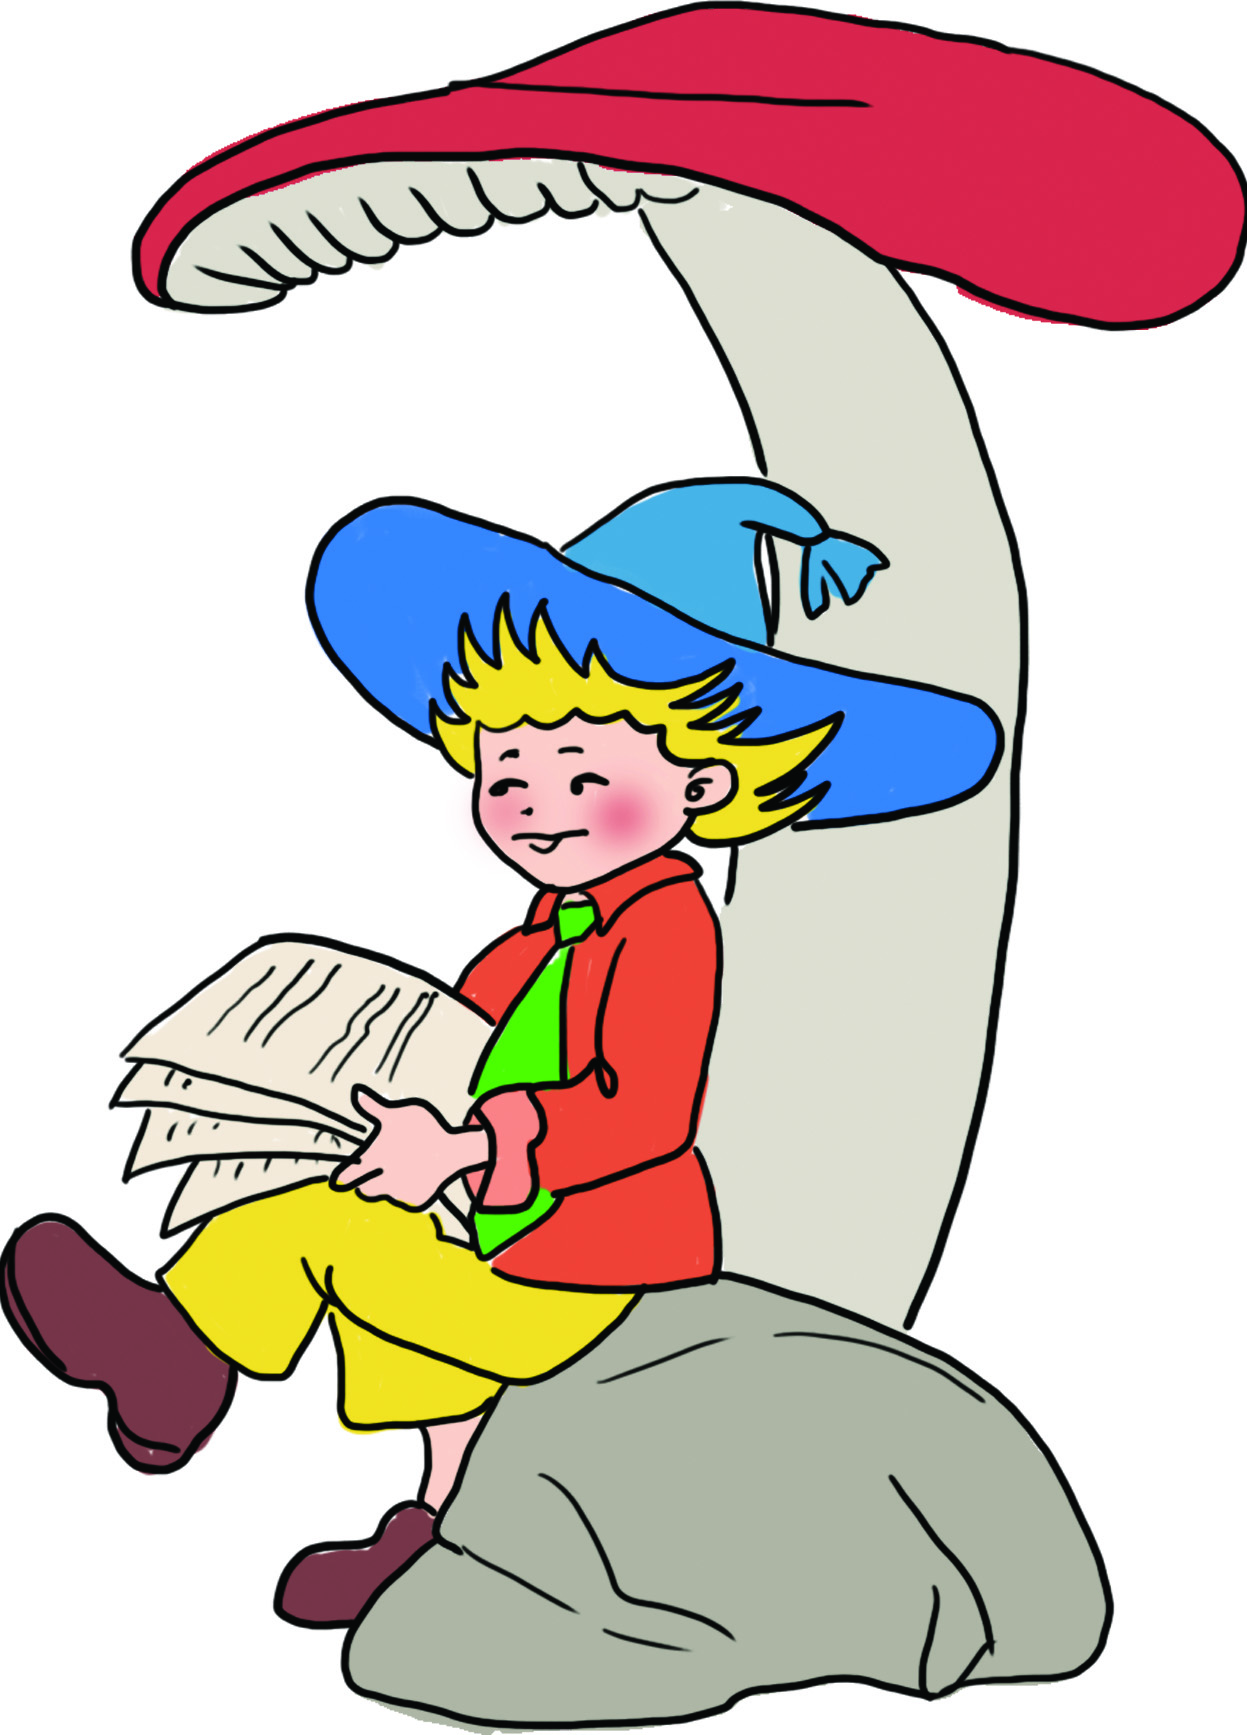
\includegraphics[width=0.35\linewidth]{Hinh22_MitDacLamToan}
		\vspace*{-10pt}
	\end{figure}
	Mít Đặc và những cô chú tí hon đáng yêu đã tham gia vào những cuộc phiêu lưu thật là thú vị phải không các em? Các em hãy đồng hành cùng các cô chú tí hon trong những cuộc phiêu lưu ấy bằng cách giải những bài toán ở trên nhé. 
	\begin{center}
		\textit{Quả cầu vĩ đại căng hơi\\
			Trời cao vút tới, bồi hồi lòng ta\\
			Tự hào như cánh chim xa\\
			Tầng không ta vượt, bay qua ruộng đồng\\
			Bay qua biển, bay qua sông\\
			Chúng ta đâu có nản lòng bạn ơi!}
	\end{center}